\documentclass[a4paper,10pt]{article}

\usepackage{geometry}
\geometry{a4paper,left=2.5cm,right=2cm,top=2.5cm,bottom=2.5cm}

\usepackage{indentfirst} % indent firts paragraph line
\setlength{\parindent}{20pt}

\usepackage{graphicx}
\graphicspath{{../output/figures/}}
% Set path for tables input
\makeatletter
\def\input@path{{../output/tables/}}
\makeatother

\usepackage{amsmath,amsthm,amsfonts,amssymb,amscd}
\usepackage{mathrsfs}
\usepackage{setspace}
\usepackage{fullpage}
\usepackage{caption}
\usepackage{tabularx}
\usepackage{enumitem}
\usepackage{url}
\usepackage{hyperref}
\usepackage{tikz}
\usepackage{multirow}
\usepackage{booktabs}
\usepackage{array}
\usepackage{wrapfig}
\usepackage{adjustbox}
\usepackage{array}
\usepackage{siunitx}
\usepackage[normalem]{ulem}
\usepackage{colortbl}
\usepackage{multirow}
\usepackage{hhline}
\usepackage{calc}
\usepackage{subcaption}	
\usepackage{float}
\usepackage{lscape}
\usepackage{threeparttable}
\usepackage{lastpage}
\usepackage{enumerate}
\usepackage{fancyhdr}
\usepackage{mathrsfs} % package for Times font style

% Citations and bibliography
\usepackage{natbib}
\bibliographystyle{chicago}

% Set spacing between lines in 1.5
\renewcommand{\baselinestretch}{1.5} 

\usepackage{hyperref}
\hypersetup{
	pdfauthor = {Bruno Paese},
	pdftitle = {The Trade Effects of Estonia's Integration into the European Community: A Structural Gravity Analysis},
	pdfkeywords = {},
	colorlinks=false
}

\title{The Trade Effects of Estonia's Integration into the European Community: A Structural Gravity Analysis}
\author{Bruno Paese\thanks{Assignment presented for the course of European Economic Integration and Regional Integration Analysis (F000954A), as part of the module of Regional Integration Analysis, under the supervision of Prof. Dr. Ruben Dewitte. Contact: bruno.paese7@gmail.com}, Gellért Turkevi--Nagy\thanks{gellert.turkevinagy@ugent.be}, and Ebenezer Sosu\thanks{ebenezer.sosu@ugent.be}}
\date{}

\begin{document}
	\maketitle
	
\section{Introduction} \label{introduction}

Since gaining independence from the Soviet Union (USSR) in 1991, Estonia has undergone one of the ``most comprehensive economic transformation(s) [...] in modern history" \citep{feldmann_soviet_2002}. The previously centralized economic system enforced by the USSR was replaced with a democratic legal framework and an independent Parliament. Privatization initiatives attracted foreign direct investment, catalyzing growth. By the late 1990s, real GDP per capita growth reached an annual rate of 10 per cent---the highest in Europe \citep{csaba_capitalist_1995,laar_leading_2008}. Economic growth and institutional developments coincided with a rise in Estonia's trade openness, too. In the early 1990s, Estonia pursued an exceptionally liberal trade policy, eliminating tariffs and non-tariff barriers, which greatly stimulated trade. However, a shift towards a multilateral approach occurred in the mid-1990s, marked by the signing of bilateral FTAs and subsequent accession to multilateral organizations such as the World Trade Organization (WTO) and the European Union (EU).

This work focuses on the effects of two pre-accession FTAs between Estonia and the European Community (EC), coming into effect in 1995 and 1998, respectively. Why is studying this integration episode especially pertient in the present context? The reason is twofold. First, it allows us to estimate the impact of Estonia's bilateral trade opening to the EC after a period when it has \textit{already} liberalized its trade policy. Consequently, a weaker impact in trade on the part of the EU would be anticipated, given Estonia's unilateral free trade stance since the early 1990s. For the EC, the main rationale behind the FTAs was to facilitate Estonia's integration into the European economy. From the Estonian perspective, the rise in trade is expected to be more profound, as it secured preferential access to the EC market \citep{feldmann_soviet_2002}. Second, it helps explore the stepwise nature of the Estonia–EC integration episode, evident in the transition from a trade-centric focus to a broader accession-oriented approach by the late 1990s. The first FTA---coming into force in 1995---primarily liberalized trade, while the second, the Association (or Europe) Agreement---entering into force in 1998---served more as a political singnalling tool for Estonia's EU accession. The distinct objectives of the two FTAs suggest that their impacts would differ: one might anticipate a more pronounced effect stemming from the initial FTA due to its narrower focus on trade liberalization.

Four key research questions arise. First, did Estonia experience an increase in trade as a result of the  integration episode? Second, is it the case that this effect was less pronounced for the EC, given Estonia's already open trade regime with zero tariffs and no non-tariff barriers? Third, do the results hold for various methodological considerations in structural gravity estimation? Lastly, can discernible differences in the magnitudes of the two FTAs studied be identified due to the differences in their aims?

While some attention has been given to the effects of pre-accession FTAs 1990s in the trade literature, no study has investigated the effects of the FTAs between Estonia and the EC \textit{per se}. The present work aims to fill this gap. It provides three key contributions that build upon antecedents. First, we demonstrate that the bilateral trade opening had a more significant impact on Estonia than on the EC. This finding confirms the hypothesis that the EC capitalized on Estonia's early adoption of liberal trade policies, resulting in the FTAs having a smaller effect on EU exports to Estonia compared to the reverse. Second, this study is the first to explicitly assess the heterogeneity of the two FTAs in the integration episode. We show that the first FTA---coming into effect in 1995---, had a more positive impact on trade flows than the second FTA of 1998. This confirms the hypothesis that the Association Agreement served more as a political and signalling tool. Further, it also serves as evidence for the shift in strategic interests for both Estonia and the EC in the mid-1990s, transitioning from bilateral trade liberalization towards expediting Estonia's integration into the EC. Third, our study employs state-of-the-art methodologies in structural gravity analysis to validate the robustness of our findings. Besides  Traditional Gravity specifications, we employ various methodological extensions and robustness checks---such as  Multilateral Resistance estimates and Poisson Pseudo Maximum Likelihood (PPML) estimation---, which evolve towards state-of-the-art structural gravity estimations.

The rest of the paper is structured as follows. Section \ref{timeline} presents the timeline of the integration episode. Based on this, Section \ref{literature} outlines the main contributions of the trade literature on the effects of Estonia's trade opening, the EC's pre-accession FTAs, and the regional context of the integration episode. To contextualize the results, Section \ref{descriptive} presents the main elements of the descriptive analysis. Section \ref{methodology} discusses the methodology. Section \ref{results} presents the empirical results of the gravity estimations, contextualizing them with insights from the descriptive analysis and existing literature. Section \ref{conclusion} concludes.

\section{Timeline of Integration Episode} \label{timeline}

Estonia's journey towards integration into the EC can be outlined in three key phases \citep{feldmann_soviet_2002}. Figure \ref{fig:timeline}  provides a chronological timeline of the integration episode.

% Timeline chart
\begin{figure}[h]
	\centering
	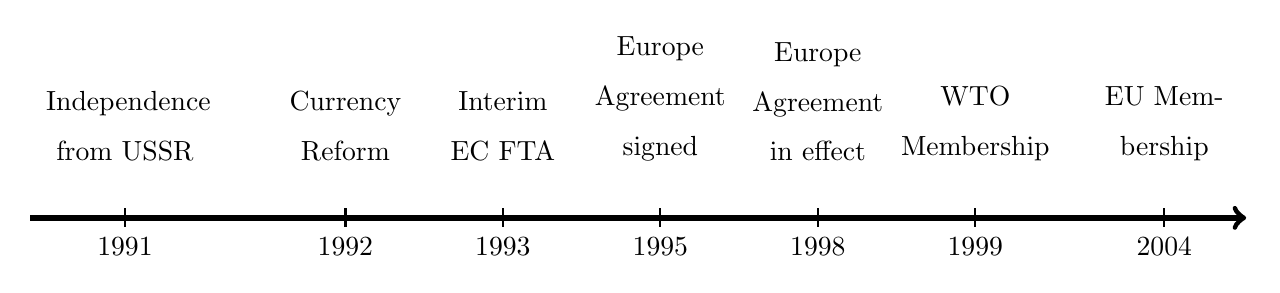
\begin{tikzpicture}[xscale=0.8,yscale=1.2]
		% Draw horizontal line; adjust line width and color here
		\draw[->, line width=2pt, color=black] (-2.5,0) -- (16.8,0); 
		% Draw events and descriptions
		\foreach \x/\event/\eventdesc in    {-1/1991/Independence from USSR,
			2.5/1992/Currency Reform,
			5/1993/Interim EC FTA,
			7.5/1995/Europe Agreement signed,
			10/1998/Europe Agreement in effect,
			12.5/1999/WTO Membership,
			15.5/2004/EU Membership} 
		{\draw[thick] (\x,0.1) -- (\x,-0.1) node[below,text width=1.5cm,align=center] {\event};
			\node[align=center,text width=2cm,anchor=south] at (\x,0.5)
			{\eventdesc};}
	\end{tikzpicture}
	\caption{Timeline of the Estonia--EC Integration Episode (1991--2004)}
	\label{fig:timeline}
\end{figure}

\subsection{Phase 1: Unilateral Opening (1991--1994)} \label{phase1}

In the early 1990s, Estonia swiftly abolished Soviet-style quotas \textit{without} converting them into tariffs \citep{feldmann_soviet_2002}. By the mid-1990s, the elimination of tariffs and non-tariff barriers led to a surge in trade. Other institutional reforms---such as the currency reform of 1992 which established the Estonian kroon pegged to the Deutsche Mark under a Currency Board---played crucial roles in enhancing productivity \citep{korhonen_currency_2000}. Additionally, significant inflows of FDI from Western countries followed the establishment of full capital mobility in 1994, contributing further to Estonia's economic growth \citep{purju_political_1996}.

\subsection{Phase 2: Bilateral Opening (1995--1998)} \label{phase2}

Starting from 1995, Estonia's approach to trade policy shifted from ultra-free trade towards regional integration through bilateral FTAs. Two such FTAs were the ones signed with the EC, coming into effect in 1995 and 1998, as shown in Figure \ref{fig:timeline}. These FTAs served a triple role for Estonia. First, they facilitated access to new export markets. This was crucial as Estonia was not a member of the General Agreement on Tariffs and Trade (GATT) and thus did not automatically receive Most Favored Nation (MFN) treatment from other countries \citep{feldmann_soviet_2002}. Second, domestically, these agreements helped cement free trade policies with partner countries. With growing pressure from agricultural interest groups pushing for protection, the FTAs helped maintain open trade relations. Third, on a political level, these agreements signaled Estonia's commitment to integrating with Western economies. The two FTAs signed with the EC---especially the second---laid a legal foundation for Estonia's eventual accession to the EU, too, and marked a shift away from dependence on Russia \citep{pisuke_estonia_1996}.

To better understand the relevance of these FTAs, we summarize their contexts and key aims in Table \ref{tab:trade_agreements} in Appendix \ref{appendix_summary}. The first agreement \textit{already} established free trade between Estonia and the EC \citep{pisuke_estonia_1996}. Customs duties and quantitative restrictions were removed, excluding some agricultural products. The Europe Agreement boasted a broader scope, preparing Estonia for EU accession. It eliminated all remaining trade barriers in agriculture \citep{westin_baltic_1998},  enabled the free movement of goods, and granted Estonian workers free movement within EU member states. The Agreement also facilitated the free movement of capital for FDI between the EC and Estonia. Crucially, it acknowledged Estonia's eventual accession as its ultimate goal \citep{soete_dissecting_2017}. This is why one would expect to see a stronger increase in trade following the first FTA, which is expected to be considerable for Estonia, as it gained access to a new export market in the EC. Conversely, the effect on EC exports to Estonia is expected to be more muted. This is because by the mid-1990s, Estonia had already adopted a liberal trade policy---abolishing tariffs and virtually all non-tariff barriers. By the time these FTAs came into effect, the EC had already capitalized on Estonia's high openness and low trade costs \citep{soete_dissecting_2017}. Importantly, Estonia's integration into the EC did not happen in isolation.  It unfolded alongside the opening of other Baltic and Eastern European nations as part of the EC's strategic motive of kickstarting their accession process \citep{westin_baltic_1998}. Alongside Estonia, the EC signed nine other Association Agreements in the region similar to the one between Estonia and the EC\footnote{Notably, three of these agreements---with the Baltic states---were all sealed in June 1995 and rendered signatories eligible for EU membership. From the EC’s perspective, signing Association Agreements served two primary purposes: signaling support for newly-independent nations and kickstarting their accession process. From the Baltic states, Estonia stood out as a regional outlier in one important aspect. Unlike Latvia and Lithuania, the effects of Estonia’s Association Agreement took hold without a transition period \cite{westin_baltic_1998}.} \citep{shen_baltic_1996}.

\subsection{Phase 3: Multi-Track Opening (1999--2004)} \label{phase3}

In the late 1990s and early 2000s, Estonia accelerated its integration into the \textit{global} community. It joined the WTO in 1999 and the EU in 2004 (Figure \ref{fig:timeline}). WTO membership provided enhanced export market access and participation in trade negotiations. EU membership solidified Estonia's position in Europe, offering institutional improvements and geopolitical protection against Russia. However, it ended its ultra-liberal trade regime, too \citep{feldmann_soviet_2002,varblane_impact_2002}.

\section{Literature Review} \label{literature}

Two early works on the effects of FTAs among Baltic and Eastern European states of the 1990s are \cite{adam_trade_2003} and \cite{martin_trade_2003}. Their key contribution is that pre-accession FTAs have been mostly successful in increasing trade flows between Eastern European and Baltic states and the EU. Still, adopting a multilateral approach---such as joining the EU---instead of the bilateral FTAs would been even more successful in increasing trade \citep{adam_trade_2003}. Importantly for the present analysis, \cite{adam_trade_2003} find that Estonia-EU trade rose \textit{more} after the first FTA entered into force in 1995 than the Europe Agreement. This is because first FTA had already liberalized much of the trade prior to the Europe Agreement, which served more as an institutional and signaling device \citep{soete_dissecting_2017}.

Building on \cite{adam_trade_2003} is \cite{benedictis_hub-and-spoke_2005}. Their main conclusion is that the increase in bilateral integration among Baltic states through the series of FTAs in the 1990s---both with the EC and each other---increased trade \textit{more between themselves} than with the EC. The main driving force of this was the fact that "reduction of trade barriers had already taken place" \citep{benedictis_hub-and-spoke_2005}. As highlighted in Section \ref{timeline}, in the case of Estonia, this was especially important. The erosion of tariffs in the 1990s prompted the EC to capitalize on cheap trade with Estonia, even before the FTAs entered into force.

As noted earlier, it was not only Estonia that signed FTAs during its gradual integration into the EU but also nine other countries in Eastern Europe. \cite{spies_trade_2009} show that \textit{all} pre-accession FTAs signed between the EU and Eastern European and Baltic states had a positive impact on trade. Importantly, this effect was strongest in the Baltic countries. Regarding methodology, they extend \cite{adam_trade_2003} and \cite{benedictis_hub-and-spoke_2005} in one important aspect. They use a larger time frame for their analysis, running from 1991 to 2003. Importantly for the present analysis, they find that the effects of the Europe Agreements entering into force in 1998 were \textit{stronger} than those of the interim agreements---contradicting \cite{adam_trade_2003}. However, this conclusion should not be extrapolated to Estonia as \cite{spies_trade_2009} do not unpack the effects of the pre-accession FTAs on a country level. Further works contextualize other aspects of the Estonia-EC integration process. \cite{fainstein_foreign_2010} find that following Estonia's independence from the USSR---even before the two FTAs---, trade flows from the USSR reoriented quickly toward to Europe, with the EU market making up around two-thirds of both Estonia's imports and exports by the mid-1990s \citep{fainstein_foreign_2010}. This reinforces the argument that the EU took advantage of the elimination of Estonian trade barriers early on.

\section{Descriptive Analysis} \label{descriptive}

In this section, we help contextualize and better interpret the empirical findings of the next section by investigating trade flows and barriers regarding the trade relations between Estonia and the EC. We use data from The International Trade and Production Database for Estimation - Release 2 (ITPD-E-R02)\footnote{See \cite{borchert_international_2022} and \cite{borchert_international_2021}.}, the World Bank's World Integrated Trade Solution (WITS) database\footnote{See \cite{world_integrated_trade_solution_estonia_2024}.}, and the Penn World Table (PWT)\footnote{See \cite{feenstra_next_2015}.}. Our data from ITPD-E-R02 ranges from 1992 to 2019, providing insights over a 27-year period, while data from the WITS database spans from 1995 to 2019. Our analysis encompasses the holistic evolution of Estonia's trade, which involves presenting total exports and imports, as well as the overall openness indicator. To contextualize trade dynamics, we present its preferred trade partners---tracking the evolution of their shares in Estonia's total exports and imports---and the trajectory of its Effectively Applied (AHS) weighted averaged tariff rate.

We start by analyzing the bigger picture of Estonia's international trade in Figure (\ref{fig:1}), which shows Estonia's total exports and imports. It can be seen that, in the early 1990s, Estonia shows a significant increase in both its exports and imports, as a result of its unilateral trade opening after the independence from the USSR. This alludes to Estonia's integration into world trade, and we can measure it by calculating an indicator of the overall openness of the Estonian economy, which is shown in Figure (\ref{fig:1.2}). There is more than one way of measuring it, and here we choose to display trade over GDP\footnote{According to \textit{A Practical Guide to Trade Policy Analysis}, the trade over GDP measure of overall openness is given by $$O^{i} = \frac{X^{i} + M^{i}}{Y^{i}},$$ where $X^{i}$, $M^{i}$ and $Y^{i}$ are respectively the country i's total exports, total imports, and GDP. The higher $O$, the more integrated country i's into world trade.}. It can be seen that there is an ascending trend in the overall openness of the Estonian economy. Especially between 1995 and 2011---except for the period of the Global Financial Crisis of 2008---, trade over GDP increased notably.

\begin{figure}[!ht]
	\centering
	\begin{subfigure}{0.49\textwidth}
		\centering 
		\includegraphics[width=1\textwidth]{EST_total_trade.pdf}
		\caption{Estonia's Total Exports and Imports.}
		\label{fig:1.1}
	\end{subfigure}
	\hfill
	\begin{subfigure}{0.49\textwidth}
		\centering
		\includegraphics[width=1\textwidth]{EST_overall_openness.pdf}
		\caption{Estonia's overall openness.}
		\label{fig:1.2}
	\end{subfigure}
	\caption{Evolution of Estonia's trade and its integration into world trade, 1992-2019. Source: ITPD-E-R02.}
	\label{fig:1}
\end{figure}

Next, we analyse Estonia's main overall trading partners in terms of shares in total trade flows\footnote{We decided to use trade shares instead of current USD because prices evolve differently and, therefore, trade shares allow us to see the decomposition of trade flows controlling for the overall increase in trade.}. Figure (\ref{fig:2}) in Appendix \ref{appendix_mtp} shows the shares of the six main partners, which are Finland, Russia, Sweden, Latvia, Germany, and Lithuania, in Estonia's total exports. Throughout the period considered, they represent approximately 50-60\% of Estonia's exports. It can be seen that, apart from Finland, all the other countries converge. The reason why these countries are the main trading partners can be explained both by the soviet past of Estonia, regarding trade with Russia, Latvia and Lithuania, and by the country's geographical proximity with them, which is also a valid argument to explain the exports to Latvia and Lithuania. Overall, Finland and Sweden are the two most important partners, even though the latter has lost importance. On the import side, Figure (\ref{fig:3}) in Appendix \ref{appendix_mtp} shows that Estonia's six main trading partners are Finland, Russia, Germany, Sweden, Lithuania and China, which represent approximately 50\% of Estonia's imports during most of the period. Differently than what we saw on the export side, here the difference between the trading partners is smaller, with also Finland---once the largest partner by a large margin---converging. In addition, China emerges as one of the main trading partners.

As previously mentioned, following its independence Estonia engaged in large-scale trade liberalisation. By the mid-1990s, import tariffs and quantitative restrictions were eliminated \citep{paas_gravity_2000}, coinciding with a fast increase in imports---and exports, too---starting in the 1990s, as already shown in Figure (\ref{fig:1.1}). To contextualise the evolution of trade barriers, we present weighted averages of AHS tariffs\footnote{The weighted AHS averages are adjusted according to their “corresponding trade value” \citep{world_integrated_trade_solution_estonia_2024}.} in Figure (\ref{fig:6}). In our analysis, it can be seen that there was a rise in the early 2000s to approximately 1\%, followed by a more substantial jump in the mid-2000s. Weighted averages were roughly one-third higher from the mid-2000s onwards, hovering around 3\% ever since around 2004. The intuition behind these trends is twofold. Firstly, weighted averages have been elevated due to larger import tariffs on products with larger weights. Secondly, the stark increase in import tariffs can be explained by Estonia joining the EU in 2004, leading to the adoption of the EU’s import schedule. This is what led to the notable increase, from the previously near-zero AHS to approximately 3\%.

\begin{figure}[!ht]
	\centering
	\includegraphics[width=0.75\linewidth]{EST_AHS.pdf}
	\caption{Estonia's Effectively Applied Tariff. Source: WITS.}
	\label{fig:6}
\end{figure}

We are mainly interested in investigating the bilateral trade flows between Estonia and the EU. Figure (\ref{fig:7}) plots the exports to the EU and imports from EU highlighting two periods, before and after Estonia accessed the bloc in 2004\footnote{It's worth mentioning that the period from 1992 to 2004 considers the 15 member-countries by 2004, even though Austria, Finland and Sweden---2 of Estonia's main trading partners---acceded the bloc in 1995, 3 years after the start of the series. In the period from 2004 to 2019, we consider in our sample all the countries (but Estonia) that joined in the fifth enlargement, i.e., Cyprus, Czech Republic, Hungary, Latvia, Lithuania, Malta, Poland, Slovakia, Slovenia, Bulgaria, Romania and Croatia.}. From the first period---before 2004---we see a gradual improvement between trade flows in both sides. However, it can be seen at the early periods that the imports from EU to Estonia increase relatively more, leading Estonia to have a trade deficit between 1992 and approximately 1999. This can be explained by Estonia's unilateral trade opening policy mentioned earlier, when the EU took advantage of the very low tariffs in Estonia during this period. However, after the first FTA between Estonia and the EC entered into force in 1995, Estonia started gaining access to European markets, and that is when exports started increasing. Additionally, as we just saw in Figure (\ref{fig:6}), Estonia started increasing tariffs in 1999, in preparation for EU accession, which is one of the causes for the decrease in imports. After 1999, it already shows a trade surplus as a result of a combination of higher tariffs and access to EU markets. From the second period---after 2004---we see a massive increase in trade flows, from both exports and imports. The reason for this notable increase is the EU's fifth enlargement, when two of Estonia's main trading partners (Latvia and Lithuania) joined.

\begin{figure}[!ht]
	\centering
	\includegraphics[width=0.9\linewidth]{Bilateral_flows.pdf}
	\caption{Bilateral trade flows between Estonia and the European Union. Source: ITPD-E-R02.}
	\label{fig:7}
\end{figure}

From the EU's perspective, the rapid increase in exports to Estonia supports the argument that the main policy objective shifted from merely boosting trade with Estonia to preparing it for accession. Trade flows were already steadily rising by the mid-1990s, indicating that the trade outlook allowed for the emphasis of the stepwise integration episode to transition from promoting free trade to initiating the process of EU accession, as trade was already experiencing swift growth. Following the first FTA, only three years later--- as seen in Figure (\ref{fig:timeline})---, the focus of the second FTA could shift toward pre-accession rather than further boosting trade.

\section{Methodology} \label{methodology}

In this section, we provide the methodological considerations of the structural gravity estimations used to assess the integration episode's impact. Here, we present the specifications and description of variables used to estimate the Traditional Gravity equations and the Free Trade Agreement effects. We also evaluate the evolution of the distance impact on trade over time---the ``Distance Puzzle" resolved---, but since our integration episode involve Estonia and the EU, distance is not a major factor in trade relations. Therefore, we decided to present our methodological considerations and results in Appendix \ref{appendix_distance}. Lastly, we use data from ITPD-E-R02 and The Dynamic Gravity Dataset\footnote{See \cite{gurevich_dynamic_2018}.}, and it is also worth mentioning that throughout all the estimations, we use data in 4-year intervals.

\subsection{Traditional Gravity Estimations} \label{traditional}

In this section, we present the specifications for the main Traditional Gravity estimations, which are the the Naïve Gravity, the Multilateral Resistances estimations, and the Poisson Pseudo Maximum Likelihood (PPML).

\subsubsection{Naïve Gravity Estimation} \label{traditional_naive}

We begin with \cite{tinbergen_shaping_1962} gravity estimation adding structural covariates. Our equation is the following:

\vspace{-1cm}

	\begin{multline*}
		ln X_{ij,t}  = \beta_{0} + \beta_{1} \ln \text{Distance}_{ij} + \beta_{2} \text{Contiguity}_{ij} + \beta_{3} \text{Common Language}_{ij} + \beta_{4} \text{Colony}_{ij} \\
		+ \beta_{5} \text{Estonia-EU 1995}_{t} + \beta_{6} \text{EU-Estonia 1995}_{t} + \beta_{7} \text{Estonia-EU 1998}_{t} + \beta_{8} \text{EU-Estonia 1998}_{t} \\
		+ \beta_{9} \text{WTO origin}_{t} + \beta_{10} \text{WTO destination}_{t} + \beta_{11} \text{EU origin}_{t} + \beta_{12} \text{EU destination}_{t} + \beta_{13} \text{FTA}_{ij,t} \\
		+ \beta_{14} \ln \text{Output}_{i,t} + \beta_{15} \ln \text{Expenditure}_{j,t} + \epsilon_{ij,t},
	\end{multline*}

\noindent where the description of our variables are the following:

\begin{spacing}{1}
	\begin{itemize}
		\item $\ln X_{ij,t}$ represents the trade flows between exporter i and importer j, at time t;
		\item $\beta_0$ is the constant term;
		\item $\ln \text{Distance}_{ij}$ is the natural log of the population-weighted bilateral distance between the two countries\footnote{Is the most widely used and robust proxy for trade costs, according to \cite{disdier_puzzling_2008}.};
		\item $\text{Contiguity}_{ij}$ is a dummy variable equal to 1 if the exporter i and importer j share a contiguous border, and 0 otherwise;
		\item $\text{Common Language}_{ij}$ is a dummy variable equal to 1 if the exporter i and importer j share at least one common language, and 0 otherwise;
		\item $\text{Colony}_{ij}$ is a dummy variable equal to 1 if the exporter i and importer j have been colonized by a common colonizer, and 0 otherwise;
		\item $\text{Estonia-EU 1995}_{t}$ is a dummy variable equal to 1 if the exporter is Estonia and the importer an EU member for years equal or greater than 1995, and 0 otherwise, at time $t$;
		\item $\text{EU-Estonia 1995}_{t}$ is a dummy variable equal to 1 if the exporter is an EU member and the importer is Estonia for years equal or greater than 1995, and 0 otherwise, at time $t$;
		\item $\text{Estonia-EU 1998}_{t}$ is a dummy variable equal to 1 if the exporter is Estonia and the importer an EU member for years equal or greater than 1998, and 0 otherwise, at time $t$;
		\item $\text{EU-Estonia 1998}_{t}$ is a dummy variable equal to 1 if the exporter is an EU member and the importer is Estonia for years equal or greater than 1998, and 0 otherwise, at time $t$;
		\item $\text{WTO origin}_{t}$ is a dummy variable equal to 1 if the origin country (exporter) is a World Trade
		Organization member at time $t$, and 0 otherwise;
		\item $\text{WTO destination}_{t}$ is a dummy variable equal to 1 if the destination country (importer) is a World Trade	Organization member at time $t$, and 0 otherwise;
		\item $\text{EU origin}_{t}$ is a dummy variable equal to 1 if the origin country (exporter) is an European Union member at time $t$, and 0 otherwise;
		\item $\text{EU destination}_{t}$ is a dummy variable equal to 1 if the destination country (importer) is an European Union member at time $t$, and 0 otherwise;
		\item $\text{FTA}_{ij,t}$ is a dummy variable for the presence of an FTA between exporter i and importer j, at time t;
		\item $\ln \text{Output}_{i,t}$ is the natural log of income of exporter i at time t (exporter country size); 
		\item $\ln \text{Expenditure}_{j,t}$ is the natural log of income of importer j at time t (importer country size);
		\item $\epsilon_{ij,t}$ is the error term correlated within country pair clusters over time.	
	\end{itemize}
\end{spacing}

The most important variables in our case are the dummies Estonia-EU and EU-Estonia. Specifically, $\text{Estonia-EU 1995}$ controls for the exports from Estonia to the EU starting from 1995, $\text{EU-Estonia 1995}$ controls for the exports from the EU to Estonia starting from 1995, and the other two dummies are the same, but instead of starting in 1995 they start in 1998. We decided to build these dummies in order to control for the bilateral flows of Estonia and the European Union, but in a way that we could simultaneously investigate which of the trade flows is the most significant, whether from Estonia to the EU, or vice versa, and which of the trade agreements has the most impact on the trade relationship, whether 1995 or 1998\footnote{That is why we used this setup instead of using two inclusive dummies that accounted for bilateral trade flows rather than unilateral.}. In this way, we believe that we will be able to test the two fundamental hypotheses of this work, namely that the 1995 FTA agreement impacted more trade flows from Estonia to the EU than the other way around, and that the 1998 FTA had a weaker impact on trade.

The advantages of using a Naive estimation is that it has high predictive power and is easy to interpret. The disadvantages are that heteroskedasticity in the data may affect the precision of the estimates; the omission of zero-trade flows in the data may bias the estimates; and the omission bias of multilateral resistance terms.

\subsubsection{Multilateral Resistances} \label{traditional_mr}

To control for multilateral resistances (MRs), we rely on two methods: using proxies for these resistances or exporter-time and importer-time fixed effects. The intuition behind controlling for MRs is that the estimates capture how remote---geographically and economically---countries are from the rest of the world. This is relevant to determine trade between countries, and so its omission may lead to biases.

In the former method, to address these biases we include proxies for both exporter and importer MR terms in the estimation, given by $\ln \text{remoteness}_{it}$ and $\ln \text{remoteness}_{jt}$. For that, we build what is called remoteness indices, which are the natural logs of output and expenditure weighted averages of bilateral distances. Our equation is then the following:

\vspace{-1cm}
	
	\begin{multline*}
		\ln X_{ij,t}  = \beta_{0} + \beta_{1} \ln \text{Distance}_{ij} + \beta_{2} \text{Contiguity}_{ij} + \beta_{3} \text{Common Language}_{ij} + \beta_{4} \text{Colony}_{ij} \\
		+ \beta_{5} \text{Estonia-EU 1995}_{t} + \beta_{6} \text{EU-Estonia 1995}_{t} + \beta_{7} \text{Estonia-EU 1998}_{t} + \beta_{8} \text{EU-Estonia 1998}_{t} \\
		+ \beta_{9} \text{WTO origin}_{t} + \beta_{10} \text{WTO destination}_{t} + \beta_{11} \text{EU origin}_{t} + \beta_{12} \text{EU destination}_{t} + \beta_{13} \text{FTA}_{ij,t} \\
		+ \beta_{14} \ln \text{Output}_{i,t} + \beta_{15} \ln \text{Expenditure}_{j,t} + \beta_{16} \ln \text{remoteness}_{it} + \beta_{17} \ln \text{remoteness}_{jt} + \epsilon_{ij,t}.
	\end{multline*}

\noindent The disadvantages of estimating with the addition of these resistance term are that, since we are still estimating by OLS, heteroskedasticity in the data may affect the precision of the estimates, and omission of zero-trade flows in the data may bias the estimates still.

However, according to the literature, the most common practice to control for MRs is with exporter and importer fixed effects \citep{feenstra_advanced_2007}. The exporter-time and importer-time fixed effects, respectively $\psi_{it}$ and $\psi_{jt}$, will absorb not only the MRs, but the size control variables too. Our specification is then the following:

\vspace{-1cm}

	\begin{multline*}
		\ln X_{ij,t}  = \beta_{1} \ln \text{Distance}_{ij} + \beta_{2} \text{Contiguity}_{ij} + \beta_{3} \text{Common Language}_{ij} + \beta_{4} \text{Colony}_{ij} \\
		+ \beta_{5} \text{Estonia-EU 1995}_{t} + \beta_{6} \text{EU-Estonia 1995}_{t} + \beta_{7} \text{Estonia-EU 1998}_{t} + \beta_{8} \text{EU-Estonia 1998}_{t} \\
		+ \beta_{9} \text{WTO origin}_{t} + \beta_{10} \text{WTO destination}_{t} + \beta_{11} \text{EU origin}_{t} + \beta_{12} \text{EU destination}_{t} + \beta_{13} \text{FTA}_{ij,t} \\
		+ \beta_{14} \ln \text{Output}_{i,t} + \beta_{15} \ln \text{Expenditure}_{j,t} + \psi_{i,t} + \psi_{j,t} + \epsilon_{ij,t}.
	\end{multline*}

\subsubsection{Poisson Pseudo Maximum Likelihood (PPML)} \label{traditional_ppml}

The PPML estimation introduced by \cite{silva_log_2006} addresses the estimation issues that arise with the use of OLS by estimating gravity in a multiplicative form. In terms of specification, the only difference from the previous gravity equation is that now we do not need to use the natural log form of trade flows. Specifically, the advantages of PPML are that its able to handle both heteroskedasticity and zero-trade in the trade data. This last point is one of the main differences between the gravity equation estimated by PPML and the others estimated by OLS, meaning that with PPML we can handle trade with value zero, which increases considerably the number of observations available. Hence, our gravity equation is the following:

\vspace{-1cm}

	\begin{multline*}
		X_{ij,t}  = \text{exp} [\beta_{1} \ln \text{Distance}_{ij} + \beta_{2} \text{Contiguity}_{ij} + \beta_{3} \text{Common Language}_{ij} + \beta_{4} \text{Colony}_{ij} \\
		+ \beta_{5} \text{Estonia-EU 1995}_{t} + \beta_{6} \text{EU-Estonia 1995}_{t} + \beta_{7} \text{Estonia-EU 1998}_{t} + \beta_{8} \text{EU-Estonia 1998}_{t} \\
		+ \beta_{9} \text{WTO origin}_{t} + \beta_{10} \text{WTO destination}_{t} + \beta_{11} \text{EU origin}_{t} + \beta_{12} \text{EU destination}_{t} + \beta_{13} \text{FTA}_{ij,t} \\
		+ \beta_{14} \ln \text{Output}_{i,t} + \beta_{15} \ln \text{Expenditure}_{j,t} + \psi_{i,t} + \psi_{j,t}]  \times \epsilon_{ij,t}.
	\end{multline*}

\subsection{Free Trade Agreement Effects} \label{fta}

In this section, we provide the specification for the equations used to assess the effects of our FTA. One thing worth mentioning is that here we decided to use only the dummies for the 1995 FTA, for reasons that will be explained in the following sections. Therefore, here we will only be looking at the effects of the first trade agreement. We provide traditional specifications, like OLS and PPML, and other specifications to account for trade-diversion from domestic sales and potential endogeneity and reverse causality. It is worth mentioning that we addressed potential non-linear and phasing-in effects, and globalization effects, but we had problems with collinearity with two of our three lag variables, and for that reason we decided not to display the results. We acknowledge that at least the non-linear and phasing-in effects would add appreciable value to our analysis.

\subsubsection{OLS and PPML Estimations} \label{fta_ols_ppml}

For the traditional OLS, the specification used is:

\vspace{-1cm}

\begin{multline*}
	\ln X_{ij,t}  = \beta_{1} \ln \text{Distance}_{ij} + \beta_{2} \text{Contiguity}_{ij} + \beta_{3} \text{Common Language}_{ij} + \beta_{4} \text{Colony}_{ij} \\
	+ \beta_{5} \text{Estonia-EU 1995}_{t} + \beta_{6} \text{EU-Estonia 1995}_{t} + \psi_{i,t} + \psi_{j,t} + \epsilon_{ij,t},
\end{multline*}

\noindent while for the state-of-the-art PPML, the specification of the gravity equation is:

\vspace{-1cm}

\begin{multline*}
	X_{ij,t} = \text{exp} [\beta_{1} \ln \text{Distance}_{ij} + \beta_{2} \text{Contiguity}_{ij} + \beta_{3} \text{Common Language}_{ij} + \beta_{4} \text{Colony}_{ij} \\
	+ \beta_{5} \text{Estonia-EU 1995}_{t} + \beta_{6} \text{EU-Estonia 1995}_{t} + \psi_{i,t} + \psi_{j,t}] \times \epsilon_{ij,t}.
\end{multline*}

\subsubsection{Trade-diversion from Domestic Sales} \label{fta_tradediversion}

The idea of this specification is to verify if our FTA caused trade to divert from domestic to international trade that was not accounted in the first place. We account for the country-specific intra-national variation in trade by
including a fixed effect, which is specified as a dummy that takes on the 3-digit ISO code of the respective country if the exporter and importer countries are the same (that is, if the trade is intra-national and not international), and \textit{International} otherwise. We estimate the gravity equation, whose specification follows below, using PPML:

\vspace{-0.7cm}

\begin{multline*}
	X_{ij,t} = \text{exp} [\beta_{1} \ln \text{Distance}_{ij} + \beta_{2} \text{Contiguity}_{ij} + \beta_{3} \text{Common Language}_{ij} + \beta_{4} \text{Colony}_{ij} \\
	+ \beta_{5} \text{Estonia-EU 1995}_{t} + \beta_{6} \text{EU-Estonia 1995}_{t} + \psi_{i,t} + \psi_{j,t} + \text{Intra-national trade}_{ii}] \times \epsilon_{ij,t}.
\end{multline*}

\subsubsection{Potential Endogeneity and Reverse Causality} \label{fta_endogeneity}

Here, we present specifications that account for reverse causality. The first strategy is to use country-pair fixed effects $\mu_{ij}$, as showed by \cite{baier_free_2007}. Then, our equation is the following:

\vspace{-0.5cm}

\begin{equation*}
	X_{ij,t} = \text{exp} [\beta_{1} \text{Estonia-EU 1995}_{t} + \beta_{2} \text{EU-Estonia 1995}_{t} + \psi_{i,t} + \psi_{j,t} + \mu_{ij}] \times \epsilon_{ij,t}.
\end{equation*}

The second specification provides a test for the previous one, to check if it correctly controls for reverse causality. This is done by constructing future values for our FTA and adding to the previous specification, as can be seen in the equation below:

\vspace{-0.5cm}

\begin{multline*}
	X_{ij,t} = \text{exp} [\beta_{1} \text{Estonia-EU 1995}_{t} + \beta_{2} \text{EU-Estonia 1995}_{t} + \beta_{3} \text{Estonia-EU 1995}_{t+4} + \beta_{4} \text{EU-Estonia 1995}_{t+4} \\
	+ \psi_{i,t} + \psi_{j,t} + \mu_{ij}] \times \epsilon_{ij,t},
\end{multline*}

\noindent where $\text{Estonia-EU 1995}_{t+4}$ and $\text{EU-Estonia 1995}_{t+4}$ are our future FTAs, and ideally they should be strictly exogenous, that is, we should not expect any of our FTAs in $t+4$ explaining trade flows in $t$. As can be seen by the functional form, both specifications are estimated by PPML.

\section{Results} \label{results}

\subsection{Traditional Gravity Estimates} \label{results_traditional}

\subsubsection{Naïve Gravity} \label{results_traditional_naive}

As expected from theory, the results from the Naïve Gravity estimates are in line with the expected signs, as shown in column (1) of Table (\ref{table_traditional_gravity}). Distance has a negative effect on trade, while contiguity, common language and colony all have positive effects, all statistically significant at the 5\% significance level. Other variables that are statistically significant and with expected results are the one corresponding to the FTAs and the ones from exporter output and importer expenditure; for instance, one percent increase in the GDP of the exporter and importer increases trade by 0.64\% and 0.61\%, respectively. On the other hand, all our dummies accounting for the WTO and the EU have negative impacts on trade, which is not expected by the literature and may be attributed to biases in the estimates. Apart from that, our results are in line with most of the standard findings in the literature on gravity estimations.

As mentioned in Section \ref{methodology}, our main variables of interest are Estonia-EU 1995, EU-Estonia 1995, Estonia-EU 1998, and EU-Estonia 1998. The coefficient of Estonia-EU 1995 is 0.765, meaning that, all else equal, the 1995 FTA agreement increases the trade flows from Estonia to the EU by 115\%. All the other coefficients---the one from EU-Estonia 1995 and the ones relative to the 1998 FTA---are not significant, neither statistically nor economically. These results are in line with our two hypotheses, that the 1995 FTA agreement impacted more trade flows from Estonia to the EU than the other way around, mostly because the EU had already capitalized on Estonia's liberal trade policy regime since the early 1990s, and that the 1998 FTA did not have a relevant impact on trade due to its essentially political nature.

\subsubsection{Multilateral Resistances} \label{results_traditional_mr}

Results of the gravity estimation accounting for multilateral resistance (MR) terms are shown in column (2) and (3) of Table (\ref{table_traditional_gravity}). As can be seen from the results, the structural gravity estimates differ from those of the naive gravity, confirming that not accounting for MR may bias the results. It is also worth mentioning that the remoteness coefficients seen in column (2) are both statistically significant. However, our MR coefficients have opposing signs, with the Exporter remoteness being relatively large and positive and the Importer remoteness being close to zero. Hence, more isolated regions tend to trade more with its neighbors, because as trade frictions increase, trade costs increase as well. 

The most noteworthy findings in our case are that the estimates of the main variables show puzzling results. In the OLS Remoteness, the importance of Estonia-EU 1995 decreased considerably, EU-Estonia 1995 now presents a positive estimate---which is the only result we would expect to see---, and Estonia-EU 1998 and EU-Estonia 1998 were removed because of collinearity. On the other hand, the OLS Fixed Effects shows that the four dummies are statistically significant at least at the 10\% significance level, but the estimates are distorted; coefficients of Estonia-EU 1995 and EU-Estonia 1995 are both negative, and the ones from Estonia-EU 1998 and EU-Estonia 1998 are positive, and large.

\subsubsection{PPML} \label{results_traditional_ppml}

As stated earlier, PPML allows us to estimate the gravity accounting for heteroskedasticity and zero trade flows. From the result in column 4, it can be seen that the sample size increases significantly, which is due to the PPML’s ability to estimate zero trade flows that were dropped from all previous OLS estimations. It can be seen that apart from Distance and FTA, all the results from the PPML differ in magnitude compared to the previous ones. As explained by \cite{larch_currency_2019}, and \cite{head_chapter_2014}, PPML and OLS weigh observations differently, which may explain the difference. Overall, Contiguity, Common language and Colony all have smaller estimates, with Colony being the only not statistically significant. The coefficient on FTA follows the same pattern as before.

Now, from our main variables, we see the results that corroborate the most with our hypotheses. First of all, the estimates related to the 1995 FTA are positive and fairly large, and even though only the one from Estonia-EU 1995 is statistically significant at the 10\% level, both of them are economically significant. The coefficients show that our FTA increases trade flows from Estonia to the EU by 149\%, while it increases the trade flows from the EU to Estonia by 115\%, which represent big effects. Secondly, both the coefficients from Estonia-EU 1998 and EU-Estonia 1998 are negative and non significant, statistically and economically. Hence, these are evidences to support the hypotheses that the 1995 FTA agreement impacted more trade flows from Estonia to the EU and that the 1998 FTA did not have a relevant impact on trade.

Therefore, to sum up, some insights arise from the Traditional Estimates. Firstly, the results from the standard gravity literature hold in most of our structural estimates. Secondly, the estimation of the gravity model using OLS and PPML provide different results due to data differences and the underlying distributions. Finally, the estimates from the Naïve Gravity and the PPML Fixed Effects are in line with our hypotheses, and for that, especially due to the results of the PPML estimation, we decided to keep Estonia-EU 1995 and EU-Estonia 1995 as our only dummies to control for the effects of the FTA agreement in the bilateral trade flows between Estonia and the EU in the following estimations. We are taking this research decision considering the Traditional Estimates, which for us provided enough evidence that the 1998 FTA had little effect on trade.


  \providecommand{\huxb}[2]{\arrayrulecolor[RGB]{#1}\global\arrayrulewidth=#2pt}
  \providecommand{\huxvb}[2]{\color[RGB]{#1}\vrule width #2pt}
  \providecommand{\huxtpad}[1]{\rule{0pt}{#1}}
  \providecommand{\huxbpad}[1]{\rule[-#1]{0pt}{#1}}

\begin{table}[htbp]
\begin{centerbox}
\begin{threeparttable}
\captionsetup{justification=centering,singlelinecheck=off}
\caption{Traditional Gravity Estimates}
 \label{table_traditional_gravity}
\setlength{\tabcolsep}{0pt}
\begin{tabularx}{1\textwidth}{p{0.3\textwidth} p{0.175\textwidth} p{0.175\textwidth} p{0.175\textwidth} p{0.175\textwidth}}


\hhline{>{\huxb{0, 0, 0}{1}}->{\huxb{0, 0, 0}{1}}->{\huxb{0, 0, 0}{1}}->{\huxb{0, 0, 0}{1}}->{\huxb{0, 0, 0}{1}}-}
\arrayrulecolor{black}

\multicolumn{1}{!{\huxvb{0, 0, 0}{0}}p{0.3\textwidth}!{\huxvb{0, 0, 0}{0}}}{\hspace{6pt}\parbox[b]{0.3\textwidth-6pt-6pt}{\huxtpad{0pt + 1em}\centering {\fontsize{9pt}{10.8pt}\selectfont }\huxbpad{0pt}}} &
\multicolumn{1}{p{0.175\textwidth}!{\huxvb{0, 0, 0}{0}}}{\hspace{6pt}\parbox[b]{0.175\textwidth-6pt-6pt}{\huxtpad{0pt + 1em}\centering {\fontsize{9pt}{10.8pt}\selectfont (1) OLS}\huxbpad{0pt}}} &
\multicolumn{1}{p{0.175\textwidth}!{\huxvb{0, 0, 0}{0}}}{\hspace{6pt}\parbox[b]{0.175\textwidth-6pt-6pt}{\huxtpad{0pt + 1em}\centering {\fontsize{9pt}{10.8pt}\selectfont (2) OLS}\huxbpad{0pt}}} &
\multicolumn{1}{p{0.175\textwidth}!{\huxvb{0, 0, 0}{0}}}{\hspace{6pt}\parbox[b]{0.175\textwidth-6pt-6pt}{\huxtpad{0pt + 1em}\centering {\fontsize{9pt}{10.8pt}\selectfont (3) OLS}\huxbpad{0pt}}} &
\multicolumn{1}{p{0.175\textwidth}!{\huxvb{0, 0, 0}{0}}}{\hspace{6pt}\parbox[b]{0.175\textwidth-6pt-6pt}{\huxtpad{0pt + 1em}\centering {\fontsize{9pt}{10.8pt}\selectfont (4) PPML}\huxbpad{0pt}}} \tabularnewline[-0.5pt]


\hhline{}
\arrayrulecolor{black}

\multicolumn{1}{!{\huxvb{0, 0, 0}{0}}p{0.3\textwidth}!{\huxvb{0, 0, 0}{0}}}{\hspace{6pt}\parbox[b]{0.3\textwidth-6pt-6pt}{\huxtpad{0pt + 1em}\centering {\fontsize{9pt}{10.8pt}\selectfont }\huxbpad{0pt}}} &
\multicolumn{1}{p{0.175\textwidth}!{\huxvb{0, 0, 0}{0}}}{\hspace{6pt}\parbox[b]{0.175\textwidth-6pt-6pt}{\huxtpad{0pt + 1em}\centering {\fontsize{9pt}{10.8pt}\selectfont Naive}\huxbpad{0pt}}} &
\multicolumn{1}{p{0.175\textwidth}!{\huxvb{0, 0, 0}{0}}}{\hspace{6pt}\parbox[b]{0.175\textwidth-6pt-6pt}{\huxtpad{0pt + 1em}\centering {\fontsize{9pt}{10.8pt}\selectfont Remoteness}\huxbpad{0pt}}} &
\multicolumn{1}{p{0.175\textwidth}!{\huxvb{0, 0, 0}{0}}}{\hspace{6pt}\parbox[b]{0.175\textwidth-6pt-6pt}{\huxtpad{0pt + 1em}\centering {\fontsize{9pt}{10.8pt}\selectfont Fixed Effects}\huxbpad{0pt}}} &
\multicolumn{1}{p{0.175\textwidth}!{\huxvb{0, 0, 0}{0}}}{\hspace{6pt}\parbox[b]{0.175\textwidth-6pt-6pt}{\huxtpad{0pt + 1em}\centering {\fontsize{9pt}{10.8pt}\selectfont Fixed Effects}\huxbpad{0pt}}} \tabularnewline[-0.5pt]


\hhline{>{\huxb{255, 255, 255}{0.4}}->{\huxb{0, 0, 0}{0.4}}->{\huxb{0, 0, 0}{0.4}}->{\huxb{0, 0, 0}{0.4}}->{\huxb{0, 0, 0}{0.4}}-}
\arrayrulecolor{black}

\multicolumn{1}{!{\huxvb{0, 0, 0}{0}}p{0.3\textwidth}!{\huxvb{0, 0, 0}{0}}}{\hspace{6pt}\parbox[b]{0.3\textwidth-6pt-6pt}{\huxtpad{0pt + 1em}\raggedright {\fontsize{9pt}{10.8pt}\selectfont Intercept}\huxbpad{0pt}}} &
\multicolumn{1}{p{0.175\textwidth}!{\huxvb{0, 0, 0}{0}}}{\hspace{6pt}\parbox[b]{0.175\textwidth-6pt-6pt}{\huxtpad{0pt + 1em}\centering {\fontsize{9pt}{10.8pt}\selectfont -6.935}\huxbpad{0pt}}} &
\multicolumn{1}{p{0.175\textwidth}!{\huxvb{0, 0, 0}{0}}}{\hspace{6pt}\parbox[b]{0.175\textwidth-6pt-6pt}{\huxtpad{0pt + 1em}\centering {\fontsize{9pt}{10.8pt}\selectfont -15.194}\huxbpad{0pt}}} &
\multicolumn{1}{p{0.175\textwidth}!{\huxvb{0, 0, 0}{0}}}{\hspace{6pt}\parbox[b]{0.175\textwidth-6pt-6pt}{\huxtpad{0pt + 1em}\centering {\fontsize{9pt}{10.8pt}\selectfont }\huxbpad{0pt}}} &
\multicolumn{1}{p{0.175\textwidth}!{\huxvb{0, 0, 0}{0}}}{\hspace{6pt}\parbox[b]{0.175\textwidth-6pt-6pt}{\huxtpad{0pt + 1em}\centering {\fontsize{9pt}{10.8pt}\selectfont }\huxbpad{0pt}}} \tabularnewline[-0.5pt]


\hhline{}
\arrayrulecolor{black}

\multicolumn{1}{!{\huxvb{0, 0, 0}{0}}p{0.3\textwidth}!{\huxvb{0, 0, 0}{0}}}{\hspace{6pt}\parbox[b]{0.3\textwidth-6pt-6pt}{\huxtpad{0pt + 1em}\raggedright {\fontsize{9pt}{10.8pt}\selectfont }\huxbpad{0pt}}} &
\multicolumn{1}{p{0.175\textwidth}!{\huxvb{0, 0, 0}{0}}}{\hspace{6pt}\parbox[b]{0.175\textwidth-6pt-6pt}{\huxtpad{0pt + 1em}\centering {\fontsize{9pt}{10.8pt}\selectfont (0.152)}\huxbpad{0pt}}} &
\multicolumn{1}{p{0.175\textwidth}!{\huxvb{0, 0, 0}{0}}}{\hspace{6pt}\parbox[b]{0.175\textwidth-6pt-6pt}{\huxtpad{0pt + 1em}\centering {\fontsize{9pt}{10.8pt}\selectfont (0.555)}\huxbpad{0pt}}} &
\multicolumn{1}{p{0.175\textwidth}!{\huxvb{0, 0, 0}{0}}}{\hspace{6pt}\parbox[b]{0.175\textwidth-6pt-6pt}{\huxtpad{0pt + 1em}\centering {\fontsize{9pt}{10.8pt}\selectfont }\huxbpad{0pt}}} &
\multicolumn{1}{p{0.175\textwidth}!{\huxvb{0, 0, 0}{0}}}{\hspace{6pt}\parbox[b]{0.175\textwidth-6pt-6pt}{\huxtpad{0pt + 1em}\centering {\fontsize{9pt}{10.8pt}\selectfont }\huxbpad{0pt}}} \tabularnewline[-0.5pt]


\hhline{}
\arrayrulecolor{black}

\multicolumn{1}{!{\huxvb{0, 0, 0}{0}}p{0.3\textwidth}!{\huxvb{0, 0, 0}{0}}}{\hspace{6pt}\parbox[b]{0.3\textwidth-6pt-6pt}{\huxtpad{0pt + 1em}\raggedright {\fontsize{9pt}{10.8pt}\selectfont ln Distance}\huxbpad{0pt}}} &
\multicolumn{1}{p{0.175\textwidth}!{\huxvb{0, 0, 0}{0}}}{\hspace{6pt}\parbox[b]{0.175\textwidth-6pt-6pt}{\huxtpad{0pt + 1em}\centering {\fontsize{9pt}{10.8pt}\selectfont -0.719}\huxbpad{0pt}}} &
\multicolumn{1}{p{0.175\textwidth}!{\huxvb{0, 0, 0}{0}}}{\hspace{6pt}\parbox[b]{0.175\textwidth-6pt-6pt}{\huxtpad{0pt + 1em}\centering {\fontsize{9pt}{10.8pt}\selectfont -0.744}\huxbpad{0pt}}} &
\multicolumn{1}{p{0.175\textwidth}!{\huxvb{0, 0, 0}{0}}}{\hspace{6pt}\parbox[b]{0.175\textwidth-6pt-6pt}{\huxtpad{0pt + 1em}\centering {\fontsize{9pt}{10.8pt}\selectfont -1.058}\huxbpad{0pt}}} &
\multicolumn{1}{p{0.175\textwidth}!{\huxvb{0, 0, 0}{0}}}{\hspace{6pt}\parbox[b]{0.175\textwidth-6pt-6pt}{\huxtpad{0pt + 1em}\centering {\fontsize{9pt}{10.8pt}\selectfont -0.738}\huxbpad{0pt}}} \tabularnewline[-0.5pt]


\hhline{}
\arrayrulecolor{black}

\multicolumn{1}{!{\huxvb{0, 0, 0}{0}}p{0.3\textwidth}!{\huxvb{0, 0, 0}{0}}}{\hspace{6pt}\parbox[b]{0.3\textwidth-6pt-6pt}{\huxtpad{0pt + 1em}\raggedright {\fontsize{9pt}{10.8pt}\selectfont }\huxbpad{0pt}}} &
\multicolumn{1}{p{0.175\textwidth}!{\huxvb{0, 0, 0}{0}}}{\hspace{6pt}\parbox[b]{0.175\textwidth-6pt-6pt}{\huxtpad{0pt + 1em}\centering {\fontsize{9pt}{10.8pt}\selectfont (0.016)}\huxbpad{0pt}}} &
\multicolumn{1}{p{0.175\textwidth}!{\huxvb{0, 0, 0}{0}}}{\hspace{6pt}\parbox[b]{0.175\textwidth-6pt-6pt}{\huxtpad{0pt + 1em}\centering {\fontsize{9pt}{10.8pt}\selectfont (0.023)}\huxbpad{0pt}}} &
\multicolumn{1}{p{0.175\textwidth}!{\huxvb{0, 0, 0}{0}}}{\hspace{6pt}\parbox[b]{0.175\textwidth-6pt-6pt}{\huxtpad{0pt + 1em}\centering {\fontsize{9pt}{10.8pt}\selectfont (0.015)}\huxbpad{0pt}}} &
\multicolumn{1}{p{0.175\textwidth}!{\huxvb{0, 0, 0}{0}}}{\hspace{6pt}\parbox[b]{0.175\textwidth-6pt-6pt}{\huxtpad{0pt + 1em}\centering {\fontsize{9pt}{10.8pt}\selectfont (0.033)}\huxbpad{0pt}}} \tabularnewline[-0.5pt]


\hhline{}
\arrayrulecolor{black}

\multicolumn{1}{!{\huxvb{0, 0, 0}{0}}p{0.3\textwidth}!{\huxvb{0, 0, 0}{0}}}{\hspace{6pt}\parbox[b]{0.3\textwidth-6pt-6pt}{\huxtpad{0pt + 1em}\raggedright {\fontsize{9pt}{10.8pt}\selectfont Contiguity}\huxbpad{0pt}}} &
\multicolumn{1}{p{0.175\textwidth}!{\huxvb{0, 0, 0}{0}}}{\hspace{6pt}\parbox[b]{0.175\textwidth-6pt-6pt}{\huxtpad{0pt + 1em}\centering {\fontsize{9pt}{10.8pt}\selectfont 1.568}\huxbpad{0pt}}} &
\multicolumn{1}{p{0.175\textwidth}!{\huxvb{0, 0, 0}{0}}}{\hspace{6pt}\parbox[b]{0.175\textwidth-6pt-6pt}{\huxtpad{0pt + 1em}\centering {\fontsize{9pt}{10.8pt}\selectfont 1.901}\huxbpad{0pt}}} &
\multicolumn{1}{p{0.175\textwidth}!{\huxvb{0, 0, 0}{0}}}{\hspace{6pt}\parbox[b]{0.175\textwidth-6pt-6pt}{\huxtpad{0pt + 1em}\centering {\fontsize{9pt}{10.8pt}\selectfont 1.080}\huxbpad{0pt}}} &
\multicolumn{1}{p{0.175\textwidth}!{\huxvb{0, 0, 0}{0}}}{\hspace{6pt}\parbox[b]{0.175\textwidth-6pt-6pt}{\huxtpad{0pt + 1em}\centering {\fontsize{9pt}{10.8pt}\selectfont 0.312}\huxbpad{0pt}}} \tabularnewline[-0.5pt]


\hhline{}
\arrayrulecolor{black}

\multicolumn{1}{!{\huxvb{0, 0, 0}{0}}p{0.3\textwidth}!{\huxvb{0, 0, 0}{0}}}{\hspace{6pt}\parbox[b]{0.3\textwidth-6pt-6pt}{\huxtpad{0pt + 1em}\raggedright {\fontsize{9pt}{10.8pt}\selectfont }\huxbpad{0pt}}} &
\multicolumn{1}{p{0.175\textwidth}!{\huxvb{0, 0, 0}{0}}}{\hspace{6pt}\parbox[b]{0.175\textwidth-6pt-6pt}{\huxtpad{0pt + 1em}\centering {\fontsize{9pt}{10.8pt}\selectfont (0.078)}\huxbpad{0pt}}} &
\multicolumn{1}{p{0.175\textwidth}!{\huxvb{0, 0, 0}{0}}}{\hspace{6pt}\parbox[b]{0.175\textwidth-6pt-6pt}{\huxtpad{0pt + 1em}\centering {\fontsize{9pt}{10.8pt}\selectfont (0.104)}\huxbpad{0pt}}} &
\multicolumn{1}{p{0.175\textwidth}!{\huxvb{0, 0, 0}{0}}}{\hspace{6pt}\parbox[b]{0.175\textwidth-6pt-6pt}{\huxtpad{0pt + 1em}\centering {\fontsize{9pt}{10.8pt}\selectfont (0.068)}\huxbpad{0pt}}} &
\multicolumn{1}{p{0.175\textwidth}!{\huxvb{0, 0, 0}{0}}}{\hspace{6pt}\parbox[b]{0.175\textwidth-6pt-6pt}{\huxtpad{0pt + 1em}\centering {\fontsize{9pt}{10.8pt}\selectfont (0.066)}\huxbpad{0pt}}} \tabularnewline[-0.5pt]


\hhline{}
\arrayrulecolor{black}

\multicolumn{1}{!{\huxvb{0, 0, 0}{0}}p{0.3\textwidth}!{\huxvb{0, 0, 0}{0}}}{\hspace{6pt}\parbox[b]{0.3\textwidth-6pt-6pt}{\huxtpad{0pt + 1em}\raggedright {\fontsize{9pt}{10.8pt}\selectfont Common language}\huxbpad{0pt}}} &
\multicolumn{1}{p{0.175\textwidth}!{\huxvb{0, 0, 0}{0}}}{\hspace{6pt}\parbox[b]{0.175\textwidth-6pt-6pt}{\huxtpad{0pt + 1em}\centering {\fontsize{9pt}{10.8pt}\selectfont 0.648}\huxbpad{0pt}}} &
\multicolumn{1}{p{0.175\textwidth}!{\huxvb{0, 0, 0}{0}}}{\hspace{6pt}\parbox[b]{0.175\textwidth-6pt-6pt}{\huxtpad{0pt + 1em}\centering {\fontsize{9pt}{10.8pt}\selectfont 0.575}\huxbpad{0pt}}} &
\multicolumn{1}{p{0.175\textwidth}!{\huxvb{0, 0, 0}{0}}}{\hspace{6pt}\parbox[b]{0.175\textwidth-6pt-6pt}{\huxtpad{0pt + 1em}\centering {\fontsize{9pt}{10.8pt}\selectfont 0.497}\huxbpad{0pt}}} &
\multicolumn{1}{p{0.175\textwidth}!{\huxvb{0, 0, 0}{0}}}{\hspace{6pt}\parbox[b]{0.175\textwidth-6pt-6pt}{\huxtpad{0pt + 1em}\centering {\fontsize{9pt}{10.8pt}\selectfont 0.251}\huxbpad{0pt}}} \tabularnewline[-0.5pt]


\hhline{}
\arrayrulecolor{black}

\multicolumn{1}{!{\huxvb{0, 0, 0}{0}}p{0.3\textwidth}!{\huxvb{0, 0, 0}{0}}}{\hspace{6pt}\parbox[b]{0.3\textwidth-6pt-6pt}{\huxtpad{0pt + 1em}\raggedright {\fontsize{9pt}{10.8pt}\selectfont }\huxbpad{0pt}}} &
\multicolumn{1}{p{0.175\textwidth}!{\huxvb{0, 0, 0}{0}}}{\hspace{6pt}\parbox[b]{0.175\textwidth-6pt-6pt}{\huxtpad{0pt + 1em}\centering {\fontsize{9pt}{10.8pt}\selectfont (0.026)}\huxbpad{0pt}}} &
\multicolumn{1}{p{0.175\textwidth}!{\huxvb{0, 0, 0}{0}}}{\hspace{6pt}\parbox[b]{0.175\textwidth-6pt-6pt}{\huxtpad{0pt + 1em}\centering {\fontsize{9pt}{10.8pt}\selectfont (0.037)}\huxbpad{0pt}}} &
\multicolumn{1}{p{0.175\textwidth}!{\huxvb{0, 0, 0}{0}}}{\hspace{6pt}\parbox[b]{0.175\textwidth-6pt-6pt}{\huxtpad{0pt + 1em}\centering {\fontsize{9pt}{10.8pt}\selectfont (0.026)}\huxbpad{0pt}}} &
\multicolumn{1}{p{0.175\textwidth}!{\huxvb{0, 0, 0}{0}}}{\hspace{6pt}\parbox[b]{0.175\textwidth-6pt-6pt}{\huxtpad{0pt + 1em}\centering {\fontsize{9pt}{10.8pt}\selectfont (0.060)}\huxbpad{0pt}}} \tabularnewline[-0.5pt]


\hhline{}
\arrayrulecolor{black}

\multicolumn{1}{!{\huxvb{0, 0, 0}{0}}p{0.3\textwidth}!{\huxvb{0, 0, 0}{0}}}{\hspace{6pt}\parbox[b]{0.3\textwidth-6pt-6pt}{\huxtpad{0pt + 1em}\raggedright {\fontsize{9pt}{10.8pt}\selectfont Colony}\huxbpad{0pt}}} &
\multicolumn{1}{p{0.175\textwidth}!{\huxvb{0, 0, 0}{0}}}{\hspace{6pt}\parbox[b]{0.175\textwidth-6pt-6pt}{\huxtpad{0pt + 1em}\centering {\fontsize{9pt}{10.8pt}\selectfont 0.358}\huxbpad{0pt}}} &
\multicolumn{1}{p{0.175\textwidth}!{\huxvb{0, 0, 0}{0}}}{\hspace{6pt}\parbox[b]{0.175\textwidth-6pt-6pt}{\huxtpad{0pt + 1em}\centering {\fontsize{9pt}{10.8pt}\selectfont 0.344}\huxbpad{0pt}}} &
\multicolumn{1}{p{0.175\textwidth}!{\huxvb{0, 0, 0}{0}}}{\hspace{6pt}\parbox[b]{0.175\textwidth-6pt-6pt}{\huxtpad{0pt + 1em}\centering {\fontsize{9pt}{10.8pt}\selectfont 0.214}\huxbpad{0pt}}} &
\multicolumn{1}{p{0.175\textwidth}!{\huxvb{0, 0, 0}{0}}}{\hspace{6pt}\parbox[b]{0.175\textwidth-6pt-6pt}{\huxtpad{0pt + 1em}\centering {\fontsize{9pt}{10.8pt}\selectfont 0.086}\huxbpad{0pt}}} \tabularnewline[-0.5pt]


\hhline{}
\arrayrulecolor{black}

\multicolumn{1}{!{\huxvb{0, 0, 0}{0}}p{0.3\textwidth}!{\huxvb{0, 0, 0}{0}}}{\hspace{6pt}\parbox[b]{0.3\textwidth-6pt-6pt}{\huxtpad{0pt + 1em}\raggedright {\fontsize{9pt}{10.8pt}\selectfont }\huxbpad{0pt}}} &
\multicolumn{1}{p{0.175\textwidth}!{\huxvb{0, 0, 0}{0}}}{\hspace{6pt}\parbox[b]{0.175\textwidth-6pt-6pt}{\huxtpad{0pt + 1em}\centering {\fontsize{9pt}{10.8pt}\selectfont (0.036)}\huxbpad{0pt}}} &
\multicolumn{1}{p{0.175\textwidth}!{\huxvb{0, 0, 0}{0}}}{\hspace{6pt}\parbox[b]{0.175\textwidth-6pt-6pt}{\huxtpad{0pt + 1em}\centering {\fontsize{9pt}{10.8pt}\selectfont (0.054)}\huxbpad{0pt}}} &
\multicolumn{1}{p{0.175\textwidth}!{\huxvb{0, 0, 0}{0}}}{\hspace{6pt}\parbox[b]{0.175\textwidth-6pt-6pt}{\huxtpad{0pt + 1em}\centering {\fontsize{9pt}{10.8pt}\selectfont (0.032)}\huxbpad{0pt}}} &
\multicolumn{1}{p{0.175\textwidth}!{\huxvb{0, 0, 0}{0}}}{\hspace{6pt}\parbox[b]{0.175\textwidth-6pt-6pt}{\huxtpad{0pt + 1em}\centering {\fontsize{9pt}{10.8pt}\selectfont (0.085)}\huxbpad{0pt}}} \tabularnewline[-0.5pt]


\hhline{}
\arrayrulecolor{black}

\multicolumn{1}{!{\huxvb{0, 0, 0}{0}}p{0.3\textwidth}!{\huxvb{0, 0, 0}{0}}}{\hspace{6pt}\parbox[b]{0.3\textwidth-6pt-6pt}{\huxtpad{0pt + 1em}\raggedright {\fontsize{9pt}{10.8pt}\selectfont Estonia-EU 1995}\huxbpad{0pt}}} &
\multicolumn{1}{p{0.175\textwidth}!{\huxvb{0, 0, 0}{0}}}{\hspace{6pt}\parbox[b]{0.175\textwidth-6pt-6pt}{\huxtpad{0pt + 1em}\centering {\fontsize{9pt}{10.8pt}\selectfont 0.765}\huxbpad{0pt}}} &
\multicolumn{1}{p{0.175\textwidth}!{\huxvb{0, 0, 0}{0}}}{\hspace{6pt}\parbox[b]{0.175\textwidth-6pt-6pt}{\huxtpad{0pt + 1em}\centering {\fontsize{9pt}{10.8pt}\selectfont 0.371}\huxbpad{0pt}}} &
\multicolumn{1}{p{0.175\textwidth}!{\huxvb{0, 0, 0}{0}}}{\hspace{6pt}\parbox[b]{0.175\textwidth-6pt-6pt}{\huxtpad{0pt + 1em}\centering {\fontsize{9pt}{10.8pt}\selectfont -0.737}\huxbpad{0pt}}} &
\multicolumn{1}{p{0.175\textwidth}!{\huxvb{0, 0, 0}{0}}}{\hspace{6pt}\parbox[b]{0.175\textwidth-6pt-6pt}{\huxtpad{0pt + 1em}\centering {\fontsize{9pt}{10.8pt}\selectfont 0.913}\huxbpad{0pt}}} \tabularnewline[-0.5pt]


\hhline{}
\arrayrulecolor{black}

\multicolumn{1}{!{\huxvb{0, 0, 0}{0}}p{0.3\textwidth}!{\huxvb{0, 0, 0}{0}}}{\hspace{6pt}\parbox[b]{0.3\textwidth-6pt-6pt}{\huxtpad{0pt + 1em}\raggedright {\fontsize{9pt}{10.8pt}\selectfont }\huxbpad{0pt}}} &
\multicolumn{1}{p{0.175\textwidth}!{\huxvb{0, 0, 0}{0}}}{\hspace{6pt}\parbox[b]{0.175\textwidth-6pt-6pt}{\huxtpad{0pt + 1em}\centering {\fontsize{9pt}{10.8pt}\selectfont (0.265)}\huxbpad{0pt}}} &
\multicolumn{1}{p{0.175\textwidth}!{\huxvb{0, 0, 0}{0}}}{\hspace{6pt}\parbox[b]{0.175\textwidth-6pt-6pt}{\huxtpad{0pt + 1em}\centering {\fontsize{9pt}{10.8pt}\selectfont (0.238)}\huxbpad{0pt}}} &
\multicolumn{1}{p{0.175\textwidth}!{\huxvb{0, 0, 0}{0}}}{\hspace{6pt}\parbox[b]{0.175\textwidth-6pt-6pt}{\huxtpad{0pt + 1em}\centering {\fontsize{9pt}{10.8pt}\selectfont (0.328)}\huxbpad{0pt}}} &
\multicolumn{1}{p{0.175\textwidth}!{\huxvb{0, 0, 0}{0}}}{\hspace{6pt}\parbox[b]{0.175\textwidth-6pt-6pt}{\huxtpad{0pt + 1em}\centering {\fontsize{9pt}{10.8pt}\selectfont (0.445)}\huxbpad{0pt}}} \tabularnewline[-0.5pt]


\hhline{}
\arrayrulecolor{black}

\multicolumn{1}{!{\huxvb{0, 0, 0}{0}}p{0.3\textwidth}!{\huxvb{0, 0, 0}{0}}}{\hspace{6pt}\parbox[b]{0.3\textwidth-6pt-6pt}{\huxtpad{0pt + 1em}\raggedright {\fontsize{9pt}{10.8pt}\selectfont EU-Estonia 1995}\huxbpad{0pt}}} &
\multicolumn{1}{p{0.175\textwidth}!{\huxvb{0, 0, 0}{0}}}{\hspace{6pt}\parbox[b]{0.175\textwidth-6pt-6pt}{\huxtpad{0pt + 1em}\centering {\fontsize{9pt}{10.8pt}\selectfont -0.165}\huxbpad{0pt}}} &
\multicolumn{1}{p{0.175\textwidth}!{\huxvb{0, 0, 0}{0}}}{\hspace{6pt}\parbox[b]{0.175\textwidth-6pt-6pt}{\huxtpad{0pt + 1em}\centering {\fontsize{9pt}{10.8pt}\selectfont 0.112}\huxbpad{0pt}}} &
\multicolumn{1}{p{0.175\textwidth}!{\huxvb{0, 0, 0}{0}}}{\hspace{6pt}\parbox[b]{0.175\textwidth-6pt-6pt}{\huxtpad{0pt + 1em}\centering {\fontsize{9pt}{10.8pt}\selectfont -0.867}\huxbpad{0pt}}} &
\multicolumn{1}{p{0.175\textwidth}!{\huxvb{0, 0, 0}{0}}}{\hspace{6pt}\parbox[b]{0.175\textwidth-6pt-6pt}{\huxtpad{0pt + 1em}\centering {\fontsize{9pt}{10.8pt}\selectfont 0.765}\huxbpad{0pt}}} \tabularnewline[-0.5pt]


\hhline{}
\arrayrulecolor{black}

\multicolumn{1}{!{\huxvb{0, 0, 0}{0}}p{0.3\textwidth}!{\huxvb{0, 0, 0}{0}}}{\hspace{6pt}\parbox[b]{0.3\textwidth-6pt-6pt}{\huxtpad{0pt + 1em}\raggedright {\fontsize{9pt}{10.8pt}\selectfont }\huxbpad{0pt}}} &
\multicolumn{1}{p{0.175\textwidth}!{\huxvb{0, 0, 0}{0}}}{\hspace{6pt}\parbox[b]{0.175\textwidth-6pt-6pt}{\huxtpad{0pt + 1em}\centering {\fontsize{9pt}{10.8pt}\selectfont (0.267)}\huxbpad{0pt}}} &
\multicolumn{1}{p{0.175\textwidth}!{\huxvb{0, 0, 0}{0}}}{\hspace{6pt}\parbox[b]{0.175\textwidth-6pt-6pt}{\huxtpad{0pt + 1em}\centering {\fontsize{9pt}{10.8pt}\selectfont (0.220)}\huxbpad{0pt}}} &
\multicolumn{1}{p{0.175\textwidth}!{\huxvb{0, 0, 0}{0}}}{\hspace{6pt}\parbox[b]{0.175\textwidth-6pt-6pt}{\huxtpad{0pt + 1em}\centering {\fontsize{9pt}{10.8pt}\selectfont (0.320)}\huxbpad{0pt}}} &
\multicolumn{1}{p{0.175\textwidth}!{\huxvb{0, 0, 0}{0}}}{\hspace{6pt}\parbox[b]{0.175\textwidth-6pt-6pt}{\huxtpad{0pt + 1em}\centering {\fontsize{9pt}{10.8pt}\selectfont (0.565)}\huxbpad{0pt}}} \tabularnewline[-0.5pt]


\hhline{}
\arrayrulecolor{black}

\multicolumn{1}{!{\huxvb{0, 0, 0}{0}}p{0.3\textwidth}!{\huxvb{0, 0, 0}{0}}}{\hspace{6pt}\parbox[b]{0.3\textwidth-6pt-6pt}{\huxtpad{0pt + 1em}\raggedright {\fontsize{9pt}{10.8pt}\selectfont Estonia-EU 1998}\huxbpad{0pt}}} &
\multicolumn{1}{p{0.175\textwidth}!{\huxvb{0, 0, 0}{0}}}{\hspace{6pt}\parbox[b]{0.175\textwidth-6pt-6pt}{\huxtpad{0pt + 1em}\centering {\fontsize{9pt}{10.8pt}\selectfont -0.394}\huxbpad{0pt}}} &
\multicolumn{1}{p{0.175\textwidth}!{\huxvb{0, 0, 0}{0}}}{\hspace{6pt}\parbox[b]{0.175\textwidth-6pt-6pt}{\huxtpad{0pt + 1em}\centering {\fontsize{9pt}{10.8pt}\selectfont }\huxbpad{0pt}}} &
\multicolumn{1}{p{0.175\textwidth}!{\huxvb{0, 0, 0}{0}}}{\hspace{6pt}\parbox[b]{0.175\textwidth-6pt-6pt}{\huxtpad{0pt + 1em}\centering {\fontsize{9pt}{10.8pt}\selectfont 1.066}\huxbpad{0pt}}} &
\multicolumn{1}{p{0.175\textwidth}!{\huxvb{0, 0, 0}{0}}}{\hspace{6pt}\parbox[b]{0.175\textwidth-6pt-6pt}{\huxtpad{0pt + 1em}\centering {\fontsize{9pt}{10.8pt}\selectfont -0.144}\huxbpad{0pt}}} \tabularnewline[-0.5pt]


\hhline{}
\arrayrulecolor{black}

\multicolumn{1}{!{\huxvb{0, 0, 0}{0}}p{0.3\textwidth}!{\huxvb{0, 0, 0}{0}}}{\hspace{6pt}\parbox[b]{0.3\textwidth-6pt-6pt}{\huxtpad{0pt + 1em}\raggedright {\fontsize{9pt}{10.8pt}\selectfont }\huxbpad{0pt}}} &
\multicolumn{1}{p{0.175\textwidth}!{\huxvb{0, 0, 0}{0}}}{\hspace{6pt}\parbox[b]{0.175\textwidth-6pt-6pt}{\huxtpad{0pt + 1em}\centering {\fontsize{9pt}{10.8pt}\selectfont (0.233)}\huxbpad{0pt}}} &
\multicolumn{1}{p{0.175\textwidth}!{\huxvb{0, 0, 0}{0}}}{\hspace{6pt}\parbox[b]{0.175\textwidth-6pt-6pt}{\huxtpad{0pt + 1em}\centering {\fontsize{9pt}{10.8pt}\selectfont }\huxbpad{0pt}}} &
\multicolumn{1}{p{0.175\textwidth}!{\huxvb{0, 0, 0}{0}}}{\hspace{6pt}\parbox[b]{0.175\textwidth-6pt-6pt}{\huxtpad{0pt + 1em}\centering {\fontsize{9pt}{10.8pt}\selectfont (0.300)}\huxbpad{0pt}}} &
\multicolumn{1}{p{0.175\textwidth}!{\huxvb{0, 0, 0}{0}}}{\hspace{6pt}\parbox[b]{0.175\textwidth-6pt-6pt}{\huxtpad{0pt + 1em}\centering {\fontsize{9pt}{10.8pt}\selectfont (0.222)}\huxbpad{0pt}}} \tabularnewline[-0.5pt]


\hhline{}
\arrayrulecolor{black}

\multicolumn{1}{!{\huxvb{0, 0, 0}{0}}p{0.3\textwidth}!{\huxvb{0, 0, 0}{0}}}{\hspace{6pt}\parbox[b]{0.3\textwidth-6pt-6pt}{\huxtpad{0pt + 1em}\raggedright {\fontsize{9pt}{10.8pt}\selectfont EU-Estonia 1998}\huxbpad{0pt}}} &
\multicolumn{1}{p{0.175\textwidth}!{\huxvb{0, 0, 0}{0}}}{\hspace{6pt}\parbox[b]{0.175\textwidth-6pt-6pt}{\huxtpad{0pt + 1em}\centering {\fontsize{9pt}{10.8pt}\selectfont 0.192}\huxbpad{0pt}}} &
\multicolumn{1}{p{0.175\textwidth}!{\huxvb{0, 0, 0}{0}}}{\hspace{6pt}\parbox[b]{0.175\textwidth-6pt-6pt}{\huxtpad{0pt + 1em}\centering {\fontsize{9pt}{10.8pt}\selectfont }\huxbpad{0pt}}} &
\multicolumn{1}{p{0.175\textwidth}!{\huxvb{0, 0, 0}{0}}}{\hspace{6pt}\parbox[b]{0.175\textwidth-6pt-6pt}{\huxtpad{0pt + 1em}\centering {\fontsize{9pt}{10.8pt}\selectfont 1.328}\huxbpad{0pt}}} &
\multicolumn{1}{p{0.175\textwidth}!{\huxvb{0, 0, 0}{0}}}{\hspace{6pt}\parbox[b]{0.175\textwidth-6pt-6pt}{\huxtpad{0pt + 1em}\centering {\fontsize{9pt}{10.8pt}\selectfont -0.241}\huxbpad{0pt}}} \tabularnewline[-0.5pt]


\hhline{}
\arrayrulecolor{black}

\multicolumn{1}{!{\huxvb{0, 0, 0}{0}}p{0.3\textwidth}!{\huxvb{0, 0, 0}{0}}}{\hspace{6pt}\parbox[b]{0.3\textwidth-6pt-6pt}{\huxtpad{0pt + 1em}\raggedright {\fontsize{9pt}{10.8pt}\selectfont }\huxbpad{0pt}}} &
\multicolumn{1}{p{0.175\textwidth}!{\huxvb{0, 0, 0}{0}}}{\hspace{6pt}\parbox[b]{0.175\textwidth-6pt-6pt}{\huxtpad{0pt + 1em}\centering {\fontsize{9pt}{10.8pt}\selectfont (0.281)}\huxbpad{0pt}}} &
\multicolumn{1}{p{0.175\textwidth}!{\huxvb{0, 0, 0}{0}}}{\hspace{6pt}\parbox[b]{0.175\textwidth-6pt-6pt}{\huxtpad{0pt + 1em}\centering {\fontsize{9pt}{10.8pt}\selectfont }\huxbpad{0pt}}} &
\multicolumn{1}{p{0.175\textwidth}!{\huxvb{0, 0, 0}{0}}}{\hspace{6pt}\parbox[b]{0.175\textwidth-6pt-6pt}{\huxtpad{0pt + 1em}\centering {\fontsize{9pt}{10.8pt}\selectfont (0.338)}\huxbpad{0pt}}} &
\multicolumn{1}{p{0.175\textwidth}!{\huxvb{0, 0, 0}{0}}}{\hspace{6pt}\parbox[b]{0.175\textwidth-6pt-6pt}{\huxtpad{0pt + 1em}\centering {\fontsize{9pt}{10.8pt}\selectfont (0.341)}\huxbpad{0pt}}} \tabularnewline[-0.5pt]


\hhline{}
\arrayrulecolor{black}

\multicolumn{1}{!{\huxvb{0, 0, 0}{0}}p{0.3\textwidth}!{\huxvb{0, 0, 0}{0}}}{\hspace{6pt}\parbox[b]{0.3\textwidth-6pt-6pt}{\huxtpad{0pt + 1em}\raggedright {\fontsize{9pt}{10.8pt}\selectfont WTO origin}\huxbpad{0pt}}} &
\multicolumn{1}{p{0.175\textwidth}!{\huxvb{0, 0, 0}{0}}}{\hspace{6pt}\parbox[b]{0.175\textwidth-6pt-6pt}{\huxtpad{0pt + 1em}\centering {\fontsize{9pt}{10.8pt}\selectfont -0.437}\huxbpad{0pt}}} &
\multicolumn{1}{p{0.175\textwidth}!{\huxvb{0, 0, 0}{0}}}{\hspace{6pt}\parbox[b]{0.175\textwidth-6pt-6pt}{\huxtpad{0pt + 1em}\centering {\fontsize{9pt}{10.8pt}\selectfont -0.304}\huxbpad{0pt}}} &
\multicolumn{1}{p{0.175\textwidth}!{\huxvb{0, 0, 0}{0}}}{\hspace{6pt}\parbox[b]{0.175\textwidth-6pt-6pt}{\huxtpad{0pt + 1em}\centering {\fontsize{9pt}{10.8pt}\selectfont }\huxbpad{0pt}}} &
\multicolumn{1}{p{0.175\textwidth}!{\huxvb{0, 0, 0}{0}}}{\hspace{6pt}\parbox[b]{0.175\textwidth-6pt-6pt}{\huxtpad{0pt + 1em}\centering {\fontsize{9pt}{10.8pt}\selectfont }\huxbpad{0pt}}} \tabularnewline[-0.5pt]


\hhline{}
\arrayrulecolor{black}

\multicolumn{1}{!{\huxvb{0, 0, 0}{0}}p{0.3\textwidth}!{\huxvb{0, 0, 0}{0}}}{\hspace{6pt}\parbox[b]{0.3\textwidth-6pt-6pt}{\huxtpad{0pt + 1em}\raggedright {\fontsize{9pt}{10.8pt}\selectfont }\huxbpad{0pt}}} &
\multicolumn{1}{p{0.175\textwidth}!{\huxvb{0, 0, 0}{0}}}{\hspace{6pt}\parbox[b]{0.175\textwidth-6pt-6pt}{\huxtpad{0pt + 1em}\centering {\fontsize{9pt}{10.8pt}\selectfont (0.021)}\huxbpad{0pt}}} &
\multicolumn{1}{p{0.175\textwidth}!{\huxvb{0, 0, 0}{0}}}{\hspace{6pt}\parbox[b]{0.175\textwidth-6pt-6pt}{\huxtpad{0pt + 1em}\centering {\fontsize{9pt}{10.8pt}\selectfont (0.041)}\huxbpad{0pt}}} &
\multicolumn{1}{p{0.175\textwidth}!{\huxvb{0, 0, 0}{0}}}{\hspace{6pt}\parbox[b]{0.175\textwidth-6pt-6pt}{\huxtpad{0pt + 1em}\centering {\fontsize{9pt}{10.8pt}\selectfont }\huxbpad{0pt}}} &
\multicolumn{1}{p{0.175\textwidth}!{\huxvb{0, 0, 0}{0}}}{\hspace{6pt}\parbox[b]{0.175\textwidth-6pt-6pt}{\huxtpad{0pt + 1em}\centering {\fontsize{9pt}{10.8pt}\selectfont }\huxbpad{0pt}}} \tabularnewline[-0.5pt]


\hhline{}
\arrayrulecolor{black}

\multicolumn{1}{!{\huxvb{0, 0, 0}{0}}p{0.3\textwidth}!{\huxvb{0, 0, 0}{0}}}{\hspace{6pt}\parbox[b]{0.3\textwidth-6pt-6pt}{\huxtpad{0pt + 1em}\raggedright {\fontsize{9pt}{10.8pt}\selectfont WTO destination}\huxbpad{0pt}}} &
\multicolumn{1}{p{0.175\textwidth}!{\huxvb{0, 0, 0}{0}}}{\hspace{6pt}\parbox[b]{0.175\textwidth-6pt-6pt}{\huxtpad{0pt + 1em}\centering {\fontsize{9pt}{10.8pt}\selectfont -0.510}\huxbpad{0pt}}} &
\multicolumn{1}{p{0.175\textwidth}!{\huxvb{0, 0, 0}{0}}}{\hspace{6pt}\parbox[b]{0.175\textwidth-6pt-6pt}{\huxtpad{0pt + 1em}\centering {\fontsize{9pt}{10.8pt}\selectfont -0.042}\huxbpad{0pt}}} &
\multicolumn{1}{p{0.175\textwidth}!{\huxvb{0, 0, 0}{0}}}{\hspace{6pt}\parbox[b]{0.175\textwidth-6pt-6pt}{\huxtpad{0pt + 1em}\centering {\fontsize{9pt}{10.8pt}\selectfont }\huxbpad{0pt}}} &
\multicolumn{1}{p{0.175\textwidth}!{\huxvb{0, 0, 0}{0}}}{\hspace{6pt}\parbox[b]{0.175\textwidth-6pt-6pt}{\huxtpad{0pt + 1em}\centering {\fontsize{9pt}{10.8pt}\selectfont }\huxbpad{0pt}}} \tabularnewline[-0.5pt]


\hhline{}
\arrayrulecolor{black}

\multicolumn{1}{!{\huxvb{0, 0, 0}{0}}p{0.3\textwidth}!{\huxvb{0, 0, 0}{0}}}{\hspace{6pt}\parbox[b]{0.3\textwidth-6pt-6pt}{\huxtpad{0pt + 1em}\raggedright {\fontsize{9pt}{10.8pt}\selectfont }\huxbpad{0pt}}} &
\multicolumn{1}{p{0.175\textwidth}!{\huxvb{0, 0, 0}{0}}}{\hspace{6pt}\parbox[b]{0.175\textwidth-6pt-6pt}{\huxtpad{0pt + 1em}\centering {\fontsize{9pt}{10.8pt}\selectfont (0.019)}\huxbpad{0pt}}} &
\multicolumn{1}{p{0.175\textwidth}!{\huxvb{0, 0, 0}{0}}}{\hspace{6pt}\parbox[b]{0.175\textwidth-6pt-6pt}{\huxtpad{0pt + 1em}\centering {\fontsize{9pt}{10.8pt}\selectfont (0.035)}\huxbpad{0pt}}} &
\multicolumn{1}{p{0.175\textwidth}!{\huxvb{0, 0, 0}{0}}}{\hspace{6pt}\parbox[b]{0.175\textwidth-6pt-6pt}{\huxtpad{0pt + 1em}\centering {\fontsize{9pt}{10.8pt}\selectfont }\huxbpad{0pt}}} &
\multicolumn{1}{p{0.175\textwidth}!{\huxvb{0, 0, 0}{0}}}{\hspace{6pt}\parbox[b]{0.175\textwidth-6pt-6pt}{\huxtpad{0pt + 1em}\centering {\fontsize{9pt}{10.8pt}\selectfont }\huxbpad{0pt}}} \tabularnewline[-0.5pt]


\hhline{}
\arrayrulecolor{black}

\multicolumn{1}{!{\huxvb{0, 0, 0}{0}}p{0.3\textwidth}!{\huxvb{0, 0, 0}{0}}}{\hspace{6pt}\parbox[b]{0.3\textwidth-6pt-6pt}{\huxtpad{0pt + 1em}\raggedright {\fontsize{9pt}{10.8pt}\selectfont EU origin}\huxbpad{0pt}}} &
\multicolumn{1}{p{0.175\textwidth}!{\huxvb{0, 0, 0}{0}}}{\hspace{6pt}\parbox[b]{0.175\textwidth-6pt-6pt}{\huxtpad{0pt + 1em}\centering {\fontsize{9pt}{10.8pt}\selectfont -0.236}\huxbpad{0pt}}} &
\multicolumn{1}{p{0.175\textwidth}!{\huxvb{0, 0, 0}{0}}}{\hspace{6pt}\parbox[b]{0.175\textwidth-6pt-6pt}{\huxtpad{0pt + 1em}\centering {\fontsize{9pt}{10.8pt}\selectfont -0.335}\huxbpad{0pt}}} &
\multicolumn{1}{p{0.175\textwidth}!{\huxvb{0, 0, 0}{0}}}{\hspace{6pt}\parbox[b]{0.175\textwidth-6pt-6pt}{\huxtpad{0pt + 1em}\centering {\fontsize{9pt}{10.8pt}\selectfont }\huxbpad{0pt}}} &
\multicolumn{1}{p{0.175\textwidth}!{\huxvb{0, 0, 0}{0}}}{\hspace{6pt}\parbox[b]{0.175\textwidth-6pt-6pt}{\huxtpad{0pt + 1em}\centering {\fontsize{9pt}{10.8pt}\selectfont }\huxbpad{0pt}}} \tabularnewline[-0.5pt]


\hhline{}
\arrayrulecolor{black}

\multicolumn{1}{!{\huxvb{0, 0, 0}{0}}p{0.3\textwidth}!{\huxvb{0, 0, 0}{0}}}{\hspace{6pt}\parbox[b]{0.3\textwidth-6pt-6pt}{\huxtpad{0pt + 1em}\raggedright {\fontsize{9pt}{10.8pt}\selectfont }\huxbpad{0pt}}} &
\multicolumn{1}{p{0.175\textwidth}!{\huxvb{0, 0, 0}{0}}}{\hspace{6pt}\parbox[b]{0.175\textwidth-6pt-6pt}{\huxtpad{0pt + 1em}\centering {\fontsize{9pt}{10.8pt}\selectfont (0.027)}\huxbpad{0pt}}} &
\multicolumn{1}{p{0.175\textwidth}!{\huxvb{0, 0, 0}{0}}}{\hspace{6pt}\parbox[b]{0.175\textwidth-6pt-6pt}{\huxtpad{0pt + 1em}\centering {\fontsize{9pt}{10.8pt}\selectfont (0.039)}\huxbpad{0pt}}} &
\multicolumn{1}{p{0.175\textwidth}!{\huxvb{0, 0, 0}{0}}}{\hspace{6pt}\parbox[b]{0.175\textwidth-6pt-6pt}{\huxtpad{0pt + 1em}\centering {\fontsize{9pt}{10.8pt}\selectfont }\huxbpad{0pt}}} &
\multicolumn{1}{p{0.175\textwidth}!{\huxvb{0, 0, 0}{0}}}{\hspace{6pt}\parbox[b]{0.175\textwidth-6pt-6pt}{\huxtpad{0pt + 1em}\centering {\fontsize{9pt}{10.8pt}\selectfont }\huxbpad{0pt}}} \tabularnewline[-0.5pt]


\hhline{}
\arrayrulecolor{black}

\multicolumn{1}{!{\huxvb{0, 0, 0}{0}}p{0.3\textwidth}!{\huxvb{0, 0, 0}{0}}}{\hspace{6pt}\parbox[b]{0.3\textwidth-6pt-6pt}{\huxtpad{0pt + 1em}\raggedright {\fontsize{9pt}{10.8pt}\selectfont EU destination}\huxbpad{0pt}}} &
\multicolumn{1}{p{0.175\textwidth}!{\huxvb{0, 0, 0}{0}}}{\hspace{6pt}\parbox[b]{0.175\textwidth-6pt-6pt}{\huxtpad{0pt + 1em}\centering {\fontsize{9pt}{10.8pt}\selectfont -0.025}\huxbpad{0pt}}} &
\multicolumn{1}{p{0.175\textwidth}!{\huxvb{0, 0, 0}{0}}}{\hspace{6pt}\parbox[b]{0.175\textwidth-6pt-6pt}{\huxtpad{0pt + 1em}\centering {\fontsize{9pt}{10.8pt}\selectfont -0.041}\huxbpad{0pt}}} &
\multicolumn{1}{p{0.175\textwidth}!{\huxvb{0, 0, 0}{0}}}{\hspace{6pt}\parbox[b]{0.175\textwidth-6pt-6pt}{\huxtpad{0pt + 1em}\centering {\fontsize{9pt}{10.8pt}\selectfont }\huxbpad{0pt}}} &
\multicolumn{1}{p{0.175\textwidth}!{\huxvb{0, 0, 0}{0}}}{\hspace{6pt}\parbox[b]{0.175\textwidth-6pt-6pt}{\huxtpad{0pt + 1em}\centering {\fontsize{9pt}{10.8pt}\selectfont }\huxbpad{0pt}}} \tabularnewline[-0.5pt]


\hhline{}
\arrayrulecolor{black}

\multicolumn{1}{!{\huxvb{0, 0, 0}{0}}p{0.3\textwidth}!{\huxvb{0, 0, 0}{0}}}{\hspace{6pt}\parbox[b]{0.3\textwidth-6pt-6pt}{\huxtpad{0pt + 1em}\raggedright {\fontsize{9pt}{10.8pt}\selectfont }\huxbpad{0pt}}} &
\multicolumn{1}{p{0.175\textwidth}!{\huxvb{0, 0, 0}{0}}}{\hspace{6pt}\parbox[b]{0.175\textwidth-6pt-6pt}{\huxtpad{0pt + 1em}\centering {\fontsize{9pt}{10.8pt}\selectfont (0.033)}\huxbpad{0pt}}} &
\multicolumn{1}{p{0.175\textwidth}!{\huxvb{0, 0, 0}{0}}}{\hspace{6pt}\parbox[b]{0.175\textwidth-6pt-6pt}{\huxtpad{0pt + 1em}\centering {\fontsize{9pt}{10.8pt}\selectfont (0.045)}\huxbpad{0pt}}} &
\multicolumn{1}{p{0.175\textwidth}!{\huxvb{0, 0, 0}{0}}}{\hspace{6pt}\parbox[b]{0.175\textwidth-6pt-6pt}{\huxtpad{0pt + 1em}\centering {\fontsize{9pt}{10.8pt}\selectfont }\huxbpad{0pt}}} &
\multicolumn{1}{p{0.175\textwidth}!{\huxvb{0, 0, 0}{0}}}{\hspace{6pt}\parbox[b]{0.175\textwidth-6pt-6pt}{\huxtpad{0pt + 1em}\centering {\fontsize{9pt}{10.8pt}\selectfont }\huxbpad{0pt}}} \tabularnewline[-0.5pt]


\hhline{}
\arrayrulecolor{black}

\multicolumn{1}{!{\huxvb{0, 0, 0}{0}}p{0.3\textwidth}!{\huxvb{0, 0, 0}{0}}}{\hspace{6pt}\parbox[b]{0.3\textwidth-6pt-6pt}{\huxtpad{0pt + 1em}\raggedright {\fontsize{9pt}{10.8pt}\selectfont FTA}\huxbpad{0pt}}} &
\multicolumn{1}{p{0.175\textwidth}!{\huxvb{0, 0, 0}{0}}}{\hspace{6pt}\parbox[b]{0.175\textwidth-6pt-6pt}{\huxtpad{0pt + 1em}\centering {\fontsize{9pt}{10.8pt}\selectfont 0.241}\huxbpad{0pt}}} &
\multicolumn{1}{p{0.175\textwidth}!{\huxvb{0, 0, 0}{0}}}{\hspace{6pt}\parbox[b]{0.175\textwidth-6pt-6pt}{\huxtpad{0pt + 1em}\centering {\fontsize{9pt}{10.8pt}\selectfont 0.420}\huxbpad{0pt}}} &
\multicolumn{1}{p{0.175\textwidth}!{\huxvb{0, 0, 0}{0}}}{\hspace{6pt}\parbox[b]{0.175\textwidth-6pt-6pt}{\huxtpad{0pt + 1em}\centering {\fontsize{9pt}{10.8pt}\selectfont 0.484}\huxbpad{0pt}}} &
\multicolumn{1}{p{0.175\textwidth}!{\huxvb{0, 0, 0}{0}}}{\hspace{6pt}\parbox[b]{0.175\textwidth-6pt-6pt}{\huxtpad{0pt + 1em}\centering {\fontsize{9pt}{10.8pt}\selectfont 0.300}\huxbpad{0pt}}} \tabularnewline[-0.5pt]


\hhline{}
\arrayrulecolor{black}

\multicolumn{1}{!{\huxvb{0, 0, 0}{0}}p{0.3\textwidth}!{\huxvb{0, 0, 0}{0}}}{\hspace{6pt}\parbox[b]{0.3\textwidth-6pt-6pt}{\huxtpad{0pt + 1em}\raggedright {\fontsize{9pt}{10.8pt}\selectfont }\huxbpad{0pt}}} &
\multicolumn{1}{p{0.175\textwidth}!{\huxvb{0, 0, 0}{0}}}{\hspace{6pt}\parbox[b]{0.175\textwidth-6pt-6pt}{\huxtpad{0pt + 1em}\centering {\fontsize{9pt}{10.8pt}\selectfont (0.036)}\huxbpad{0pt}}} &
\multicolumn{1}{p{0.175\textwidth}!{\huxvb{0, 0, 0}{0}}}{\hspace{6pt}\parbox[b]{0.175\textwidth-6pt-6pt}{\huxtpad{0pt + 1em}\centering {\fontsize{9pt}{10.8pt}\selectfont (0.054)}\huxbpad{0pt}}} &
\multicolumn{1}{p{0.175\textwidth}!{\huxvb{0, 0, 0}{0}}}{\hspace{6pt}\parbox[b]{0.175\textwidth-6pt-6pt}{\huxtpad{0pt + 1em}\centering {\fontsize{9pt}{10.8pt}\selectfont (0.030)}\huxbpad{0pt}}} &
\multicolumn{1}{p{0.175\textwidth}!{\huxvb{0, 0, 0}{0}}}{\hspace{6pt}\parbox[b]{0.175\textwidth-6pt-6pt}{\huxtpad{0pt + 1em}\centering {\fontsize{9pt}{10.8pt}\selectfont (0.060)}\huxbpad{0pt}}} \tabularnewline[-0.5pt]


\hhline{}
\arrayrulecolor{black}

\multicolumn{1}{!{\huxvb{0, 0, 0}{0}}p{0.3\textwidth}!{\huxvb{0, 0, 0}{0}}}{\hspace{6pt}\parbox[b]{0.3\textwidth-6pt-6pt}{\huxtpad{0pt + 1em}\raggedright {\fontsize{9pt}{10.8pt}\selectfont ln Output}\huxbpad{0pt}}} &
\multicolumn{1}{p{0.175\textwidth}!{\huxvb{0, 0, 0}{0}}}{\hspace{6pt}\parbox[b]{0.175\textwidth-6pt-6pt}{\huxtpad{0pt + 1em}\centering {\fontsize{9pt}{10.8pt}\selectfont 0.643}\huxbpad{0pt}}} &
\multicolumn{1}{p{0.175\textwidth}!{\huxvb{0, 0, 0}{0}}}{\hspace{6pt}\parbox[b]{0.175\textwidth-6pt-6pt}{\huxtpad{0pt + 1em}\centering {\fontsize{9pt}{10.8pt}\selectfont 0.582}\huxbpad{0pt}}} &
\multicolumn{1}{p{0.175\textwidth}!{\huxvb{0, 0, 0}{0}}}{\hspace{6pt}\parbox[b]{0.175\textwidth-6pt-6pt}{\huxtpad{0pt + 1em}\centering {\fontsize{9pt}{10.8pt}\selectfont }\huxbpad{0pt}}} &
\multicolumn{1}{p{0.175\textwidth}!{\huxvb{0, 0, 0}{0}}}{\hspace{6pt}\parbox[b]{0.175\textwidth-6pt-6pt}{\huxtpad{0pt + 1em}\centering {\fontsize{9pt}{10.8pt}\selectfont }\huxbpad{0pt}}} \tabularnewline[-0.5pt]


\hhline{}
\arrayrulecolor{black}

\multicolumn{1}{!{\huxvb{0, 0, 0}{0}}p{0.3\textwidth}!{\huxvb{0, 0, 0}{0}}}{\hspace{6pt}\parbox[b]{0.3\textwidth-6pt-6pt}{\huxtpad{0pt + 1em}\raggedright {\fontsize{9pt}{10.8pt}\selectfont }\huxbpad{0pt}}} &
\multicolumn{1}{p{0.175\textwidth}!{\huxvb{0, 0, 0}{0}}}{\hspace{6pt}\parbox[b]{0.175\textwidth-6pt-6pt}{\huxtpad{0pt + 1em}\centering {\fontsize{9pt}{10.8pt}\selectfont (0.004)}\huxbpad{0pt}}} &
\multicolumn{1}{p{0.175\textwidth}!{\huxvb{0, 0, 0}{0}}}{\hspace{6pt}\parbox[b]{0.175\textwidth-6pt-6pt}{\huxtpad{0pt + 1em}\centering {\fontsize{9pt}{10.8pt}\selectfont (0.007)}\huxbpad{0pt}}} &
\multicolumn{1}{p{0.175\textwidth}!{\huxvb{0, 0, 0}{0}}}{\hspace{6pt}\parbox[b]{0.175\textwidth-6pt-6pt}{\huxtpad{0pt + 1em}\centering {\fontsize{9pt}{10.8pt}\selectfont }\huxbpad{0pt}}} &
\multicolumn{1}{p{0.175\textwidth}!{\huxvb{0, 0, 0}{0}}}{\hspace{6pt}\parbox[b]{0.175\textwidth-6pt-6pt}{\huxtpad{0pt + 1em}\centering {\fontsize{9pt}{10.8pt}\selectfont }\huxbpad{0pt}}} \tabularnewline[-0.5pt]


\hhline{}
\arrayrulecolor{black}

\multicolumn{1}{!{\huxvb{0, 0, 0}{0}}p{0.3\textwidth}!{\huxvb{0, 0, 0}{0}}}{\hspace{6pt}\parbox[b]{0.3\textwidth-6pt-6pt}{\huxtpad{0pt + 1em}\raggedright {\fontsize{9pt}{10.8pt}\selectfont ln Expenditure}\huxbpad{0pt}}} &
\multicolumn{1}{p{0.175\textwidth}!{\huxvb{0, 0, 0}{0}}}{\hspace{6pt}\parbox[b]{0.175\textwidth-6pt-6pt}{\huxtpad{0pt + 1em}\centering {\fontsize{9pt}{10.8pt}\selectfont 0.610}\huxbpad{0pt}}} &
\multicolumn{1}{p{0.175\textwidth}!{\huxvb{0, 0, 0}{0}}}{\hspace{6pt}\parbox[b]{0.175\textwidth-6pt-6pt}{\huxtpad{0pt + 1em}\centering {\fontsize{9pt}{10.8pt}\selectfont 0.637}\huxbpad{0pt}}} &
\multicolumn{1}{p{0.175\textwidth}!{\huxvb{0, 0, 0}{0}}}{\hspace{6pt}\parbox[b]{0.175\textwidth-6pt-6pt}{\huxtpad{0pt + 1em}\centering {\fontsize{9pt}{10.8pt}\selectfont }\huxbpad{0pt}}} &
\multicolumn{1}{p{0.175\textwidth}!{\huxvb{0, 0, 0}{0}}}{\hspace{6pt}\parbox[b]{0.175\textwidth-6pt-6pt}{\huxtpad{0pt + 1em}\centering {\fontsize{9pt}{10.8pt}\selectfont }\huxbpad{0pt}}} \tabularnewline[-0.5pt]


\hhline{}
\arrayrulecolor{black}

\multicolumn{1}{!{\huxvb{0, 0, 0}{0}}p{0.3\textwidth}!{\huxvb{0, 0, 0}{0}}}{\hspace{6pt}\parbox[b]{0.3\textwidth-6pt-6pt}{\huxtpad{0pt + 1em}\raggedright {\fontsize{9pt}{10.8pt}\selectfont }\huxbpad{0pt}}} &
\multicolumn{1}{p{0.175\textwidth}!{\huxvb{0, 0, 0}{0}}}{\hspace{6pt}\parbox[b]{0.175\textwidth-6pt-6pt}{\huxtpad{0pt + 1em}\centering {\fontsize{9pt}{10.8pt}\selectfont (0.005)}\huxbpad{0pt}}} &
\multicolumn{1}{p{0.175\textwidth}!{\huxvb{0, 0, 0}{0}}}{\hspace{6pt}\parbox[b]{0.175\textwidth-6pt-6pt}{\huxtpad{0pt + 1em}\centering {\fontsize{9pt}{10.8pt}\selectfont (0.007)}\huxbpad{0pt}}} &
\multicolumn{1}{p{0.175\textwidth}!{\huxvb{0, 0, 0}{0}}}{\hspace{6pt}\parbox[b]{0.175\textwidth-6pt-6pt}{\huxtpad{0pt + 1em}\centering {\fontsize{9pt}{10.8pt}\selectfont }\huxbpad{0pt}}} &
\multicolumn{1}{p{0.175\textwidth}!{\huxvb{0, 0, 0}{0}}}{\hspace{6pt}\parbox[b]{0.175\textwidth-6pt-6pt}{\huxtpad{0pt + 1em}\centering {\fontsize{9pt}{10.8pt}\selectfont }\huxbpad{0pt}}} \tabularnewline[-0.5pt]


\hhline{}
\arrayrulecolor{black}

\multicolumn{1}{!{\huxvb{0, 0, 0}{0}}p{0.3\textwidth}!{\huxvb{0, 0, 0}{0}}}{\hspace{6pt}\parbox[b]{0.3\textwidth-6pt-6pt}{\huxtpad{0pt + 1em}\raggedright {\fontsize{9pt}{10.8pt}\selectfont Exporter remoteness}\huxbpad{0pt}}} &
\multicolumn{1}{p{0.175\textwidth}!{\huxvb{0, 0, 0}{0}}}{\hspace{6pt}\parbox[b]{0.175\textwidth-6pt-6pt}{\huxtpad{0pt + 1em}\centering {\fontsize{9pt}{10.8pt}\selectfont }\huxbpad{0pt}}} &
\multicolumn{1}{p{0.175\textwidth}!{\huxvb{0, 0, 0}{0}}}{\hspace{6pt}\parbox[b]{0.175\textwidth-6pt-6pt}{\huxtpad{0pt + 1em}\centering {\fontsize{9pt}{10.8pt}\selectfont 0.262}\huxbpad{0pt}}} &
\multicolumn{1}{p{0.175\textwidth}!{\huxvb{0, 0, 0}{0}}}{\hspace{6pt}\parbox[b]{0.175\textwidth-6pt-6pt}{\huxtpad{0pt + 1em}\centering {\fontsize{9pt}{10.8pt}\selectfont }\huxbpad{0pt}}} &
\multicolumn{1}{p{0.175\textwidth}!{\huxvb{0, 0, 0}{0}}}{\hspace{6pt}\parbox[b]{0.175\textwidth-6pt-6pt}{\huxtpad{0pt + 1em}\centering {\fontsize{9pt}{10.8pt}\selectfont }\huxbpad{0pt}}} \tabularnewline[-0.5pt]


\hhline{}
\arrayrulecolor{black}

\multicolumn{1}{!{\huxvb{0, 0, 0}{0}}p{0.3\textwidth}!{\huxvb{0, 0, 0}{0}}}{\hspace{6pt}\parbox[b]{0.3\textwidth-6pt-6pt}{\huxtpad{0pt + 1em}\raggedright {\fontsize{9pt}{10.8pt}\selectfont }\huxbpad{0pt}}} &
\multicolumn{1}{p{0.175\textwidth}!{\huxvb{0, 0, 0}{0}}}{\hspace{6pt}\parbox[b]{0.175\textwidth-6pt-6pt}{\huxtpad{0pt + 1em}\centering {\fontsize{9pt}{10.8pt}\selectfont }\huxbpad{0pt}}} &
\multicolumn{1}{p{0.175\textwidth}!{\huxvb{0, 0, 0}{0}}}{\hspace{6pt}\parbox[b]{0.175\textwidth-6pt-6pt}{\huxtpad{0pt + 1em}\centering {\fontsize{9pt}{10.8pt}\selectfont (0.014)}\huxbpad{0pt}}} &
\multicolumn{1}{p{0.175\textwidth}!{\huxvb{0, 0, 0}{0}}}{\hspace{6pt}\parbox[b]{0.175\textwidth-6pt-6pt}{\huxtpad{0pt + 1em}\centering {\fontsize{9pt}{10.8pt}\selectfont }\huxbpad{0pt}}} &
\multicolumn{1}{p{0.175\textwidth}!{\huxvb{0, 0, 0}{0}}}{\hspace{6pt}\parbox[b]{0.175\textwidth-6pt-6pt}{\huxtpad{0pt + 1em}\centering {\fontsize{9pt}{10.8pt}\selectfont }\huxbpad{0pt}}} \tabularnewline[-0.5pt]


\hhline{}
\arrayrulecolor{black}

\multicolumn{1}{!{\huxvb{0, 0, 0}{0}}p{0.3\textwidth}!{\huxvb{0, 0, 0}{0}}}{\hspace{6pt}\parbox[b]{0.3\textwidth-6pt-6pt}{\huxtpad{0pt + 1em}\raggedright {\fontsize{9pt}{10.8pt}\selectfont Importer remoteness}\huxbpad{0pt}}} &
\multicolumn{1}{p{0.175\textwidth}!{\huxvb{0, 0, 0}{0}}}{\hspace{6pt}\parbox[b]{0.175\textwidth-6pt-6pt}{\huxtpad{0pt + 1em}\centering {\fontsize{9pt}{10.8pt}\selectfont }\huxbpad{0pt}}} &
\multicolumn{1}{p{0.175\textwidth}!{\huxvb{0, 0, 0}{0}}}{\hspace{6pt}\parbox[b]{0.175\textwidth-6pt-6pt}{\huxtpad{0pt + 1em}\centering {\fontsize{9pt}{10.8pt}\selectfont -0.023}\huxbpad{0pt}}} &
\multicolumn{1}{p{0.175\textwidth}!{\huxvb{0, 0, 0}{0}}}{\hspace{6pt}\parbox[b]{0.175\textwidth-6pt-6pt}{\huxtpad{0pt + 1em}\centering {\fontsize{9pt}{10.8pt}\selectfont }\huxbpad{0pt}}} &
\multicolumn{1}{p{0.175\textwidth}!{\huxvb{0, 0, 0}{0}}}{\hspace{6pt}\parbox[b]{0.175\textwidth-6pt-6pt}{\huxtpad{0pt + 1em}\centering {\fontsize{9pt}{10.8pt}\selectfont }\huxbpad{0pt}}} \tabularnewline[-0.5pt]


\hhline{}
\arrayrulecolor{black}

\multicolumn{1}{!{\huxvb{0, 0, 0}{0}}p{0.3\textwidth}!{\huxvb{0, 0, 0}{0}}}{\hspace{6pt}\parbox[b]{0.3\textwidth-6pt-6pt}{\huxtpad{0pt + 1em}\raggedright {\fontsize{9pt}{10.8pt}\selectfont }\huxbpad{0pt}}} &
\multicolumn{1}{p{0.175\textwidth}!{\huxvb{0, 0, 0}{0}}}{\hspace{6pt}\parbox[b]{0.175\textwidth-6pt-6pt}{\huxtpad{0pt + 1em}\centering {\fontsize{9pt}{10.8pt}\selectfont }\huxbpad{0pt}}} &
\multicolumn{1}{p{0.175\textwidth}!{\huxvb{0, 0, 0}{0}}}{\hspace{6pt}\parbox[b]{0.175\textwidth-6pt-6pt}{\huxtpad{0pt + 1em}\centering {\fontsize{9pt}{10.8pt}\selectfont (0.008)}\huxbpad{0pt}}} &
\multicolumn{1}{p{0.175\textwidth}!{\huxvb{0, 0, 0}{0}}}{\hspace{6pt}\parbox[b]{0.175\textwidth-6pt-6pt}{\huxtpad{0pt + 1em}\centering {\fontsize{9pt}{10.8pt}\selectfont }\huxbpad{0pt}}} &
\multicolumn{1}{p{0.175\textwidth}!{\huxvb{0, 0, 0}{0}}}{\hspace{6pt}\parbox[b]{0.175\textwidth-6pt-6pt}{\huxtpad{0pt + 1em}\centering {\fontsize{9pt}{10.8pt}\selectfont }\huxbpad{0pt}}} \tabularnewline[-0.5pt]


\hhline{>{\huxb{255, 255, 255}{0.4}}->{\huxb{0, 0, 0}{0.4}}->{\huxb{0, 0, 0}{0.4}}->{\huxb{0, 0, 0}{0.4}}->{\huxb{0, 0, 0}{0.4}}-}
\arrayrulecolor{black}

\multicolumn{1}{!{\huxvb{0, 0, 0}{0}}p{0.3\textwidth}!{\huxvb{0, 0, 0}{0}}}{\hspace{6pt}\parbox[b]{0.3\textwidth-6pt-6pt}{\huxtpad{0pt + 1em}\raggedright {\fontsize{9pt}{10.8pt}\selectfont N}\huxbpad{0pt}}} &
\multicolumn{1}{p{0.175\textwidth}!{\huxvb{0, 0, 0}{0}}}{\hspace{6pt}\parbox[b]{0.175\textwidth-6pt-6pt}{\huxtpad{0pt + 1em}\centering {\fontsize{9pt}{10.8pt}\selectfont 339357}\huxbpad{0pt}}} &
\multicolumn{1}{p{0.175\textwidth}!{\huxvb{0, 0, 0}{0}}}{\hspace{6pt}\parbox[b]{0.175\textwidth-6pt-6pt}{\huxtpad{0pt + 1em}\centering {\fontsize{9pt}{10.8pt}\selectfont 126740}\huxbpad{0pt}}} &
\multicolumn{1}{p{0.175\textwidth}!{\huxvb{0, 0, 0}{0}}}{\hspace{6pt}\parbox[b]{0.175\textwidth-6pt-6pt}{\huxtpad{0pt + 1em}\centering {\fontsize{9pt}{10.8pt}\selectfont 339357}\huxbpad{0pt}}} &
\multicolumn{1}{p{0.175\textwidth}!{\huxvb{0, 0, 0}{0}}}{\hspace{6pt}\parbox[b]{0.175\textwidth-6pt-6pt}{\huxtpad{0pt + 1em}\centering {\fontsize{9pt}{10.8pt}\selectfont 631080}\huxbpad{0pt}}} \tabularnewline[-0.5pt]


\hhline{}
\arrayrulecolor{black}

\multicolumn{1}{!{\huxvb{0, 0, 0}{0}}p{0.3\textwidth}!{\huxvb{0, 0, 0}{0}}}{\hspace{6pt}\parbox[b]{0.3\textwidth-6pt-6pt}{\huxtpad{0pt + 1em}\raggedright {\fontsize{9pt}{10.8pt}\selectfont R2}\huxbpad{0pt}}} &
\multicolumn{1}{p{0.175\textwidth}!{\huxvb{0, 0, 0}{0}}}{\hspace{6pt}\parbox[b]{0.175\textwidth-6pt-6pt}{\huxtpad{0pt + 1em}\centering {\fontsize{9pt}{10.8pt}\selectfont 0}\huxbpad{0pt}}} &
\multicolumn{1}{p{0.175\textwidth}!{\huxvb{0, 0, 0}{0}}}{\hspace{6pt}\parbox[b]{0.175\textwidth-6pt-6pt}{\huxtpad{0pt + 1em}\centering {\fontsize{9pt}{10.8pt}\selectfont 0}\huxbpad{0pt}}} &
\multicolumn{1}{p{0.175\textwidth}!{\huxvb{0, 0, 0}{0}}}{\hspace{6pt}\parbox[b]{0.175\textwidth-6pt-6pt}{\huxtpad{0pt + 1em}\centering {\fontsize{9pt}{10.8pt}\selectfont 0}\huxbpad{0pt}}} &
\multicolumn{1}{p{0.175\textwidth}!{\huxvb{0, 0, 0}{0}}}{\hspace{6pt}\parbox[b]{0.175\textwidth-6pt-6pt}{\huxtpad{0pt + 1em}\centering {\fontsize{9pt}{10.8pt}\selectfont }\huxbpad{0pt}}} \tabularnewline[-0.5pt]


\hhline{}
\arrayrulecolor{black}

\multicolumn{1}{!{\huxvb{0, 0, 0}{0}}p{0.3\textwidth}!{\huxvb{0, 0, 0}{0}}}{\hspace{6pt}\parbox[b]{0.3\textwidth-6pt-6pt}{\huxtpad{0pt + 1em}\raggedright {\fontsize{9pt}{10.8pt}\selectfont logLik}\huxbpad{0pt}}} &
\multicolumn{1}{p{0.175\textwidth}!{\huxvb{0, 0, 0}{0}}}{\hspace{6pt}\parbox[b]{0.175\textwidth-6pt-6pt}{\huxtpad{0pt + 1em}\centering {\fontsize{9pt}{10.8pt}\selectfont -886509.864}\huxbpad{0pt}}} &
\multicolumn{1}{p{0.175\textwidth}!{\huxvb{0, 0, 0}{0}}}{\hspace{6pt}\parbox[b]{0.175\textwidth-6pt-6pt}{\huxtpad{0pt + 1em}\centering {\fontsize{9pt}{10.8pt}\selectfont -332080.949}\huxbpad{0pt}}} &
\multicolumn{1}{p{0.175\textwidth}!{\huxvb{0, 0, 0}{0}}}{\hspace{6pt}\parbox[b]{0.175\textwidth-6pt-6pt}{\huxtpad{0pt + 1em}\centering {\fontsize{9pt}{10.8pt}\selectfont -862612.746}\huxbpad{0pt}}} &
\multicolumn{1}{p{0.175\textwidth}!{\huxvb{0, 0, 0}{0}}}{\hspace{6pt}\parbox[b]{0.175\textwidth-6pt-6pt}{\huxtpad{0pt + 1em}\centering {\fontsize{9pt}{10.8pt}\selectfont -85799593.393}\huxbpad{0pt}}} \tabularnewline[-0.5pt]


\hhline{}
\arrayrulecolor{black}

\multicolumn{1}{!{\huxvb{0, 0, 0}{0}}p{0.3\textwidth}!{\huxvb{0, 0, 0}{0}}}{\hspace{6pt}\parbox[b]{0.3\textwidth-6pt-6pt}{\huxtpad{0pt + 1em}\raggedright {\fontsize{9pt}{10.8pt}\selectfont AIC}\huxbpad{0pt}}} &
\multicolumn{1}{p{0.175\textwidth}!{\huxvb{0, 0, 0}{0}}}{\hspace{6pt}\parbox[b]{0.175\textwidth-6pt-6pt}{\huxtpad{0pt + 1em}\centering {\fontsize{9pt}{10.8pt}\selectfont 1773051.729}\huxbpad{0pt}}} &
\multicolumn{1}{p{0.175\textwidth}!{\huxvb{0, 0, 0}{0}}}{\hspace{6pt}\parbox[b]{0.175\textwidth-6pt-6pt}{\huxtpad{0pt + 1em}\centering {\fontsize{9pt}{10.8pt}\selectfont 664193.898}\huxbpad{0pt}}} &
\multicolumn{1}{p{0.175\textwidth}!{\huxvb{0, 0, 0}{0}}}{\hspace{6pt}\parbox[b]{0.175\textwidth-6pt-6pt}{\huxtpad{0pt + 1em}\centering {\fontsize{9pt}{10.8pt}\selectfont 1731689.492}\huxbpad{0pt}}} &
\multicolumn{1}{p{0.175\textwidth}!{\huxvb{0, 0, 0}{0}}}{\hspace{6pt}\parbox[b]{0.175\textwidth-6pt-6pt}{\huxtpad{0pt + 1em}\centering {\fontsize{9pt}{10.8pt}\selectfont 171605650.786}\huxbpad{0pt}}} \tabularnewline[-0.5pt]


\hhline{}
\arrayrulecolor{black}

\multicolumn{1}{!{\huxvb{0, 0, 0}{0}}p{0.3\textwidth}!{\huxvb{0, 0, 0}{0}}}{\hspace{6pt}\parbox[b]{0.3\textwidth-6pt-6pt}{\huxtpad{0pt + 1em}\raggedright {\fontsize{9pt}{10.8pt}\selectfont Exporter-time fixed effects}\huxbpad{0pt}}} &
\multicolumn{1}{p{0.175\textwidth}!{\huxvb{0, 0, 0}{0}}}{\hspace{6pt}\parbox[b]{0.175\textwidth-6pt-6pt}{\huxtpad{0pt + 1em}\centering {\fontsize{9pt}{10.8pt}\selectfont No}\huxbpad{0pt}}} &
\multicolumn{1}{p{0.175\textwidth}!{\huxvb{0, 0, 0}{0}}}{\hspace{6pt}\parbox[b]{0.175\textwidth-6pt-6pt}{\huxtpad{0pt + 1em}\centering {\fontsize{9pt}{10.8pt}\selectfont No}\huxbpad{0pt}}} &
\multicolumn{1}{p{0.175\textwidth}!{\huxvb{0, 0, 0}{0}}}{\hspace{6pt}\parbox[b]{0.175\textwidth-6pt-6pt}{\huxtpad{0pt + 1em}\centering {\fontsize{9pt}{10.8pt}\selectfont Yes}\huxbpad{0pt}}} &
\multicolumn{1}{p{0.175\textwidth}!{\huxvb{0, 0, 0}{0}}}{\hspace{6pt}\parbox[b]{0.175\textwidth-6pt-6pt}{\huxtpad{0pt + 1em}\centering {\fontsize{9pt}{10.8pt}\selectfont Yes}\huxbpad{0pt}}} \tabularnewline[-0.5pt]


\hhline{}
\arrayrulecolor{black}

\multicolumn{1}{!{\huxvb{0, 0, 0}{0}}p{0.3\textwidth}!{\huxvb{0, 0, 0}{0}}}{\hspace{6pt}\parbox[b]{0.3\textwidth-6pt-6pt}{\huxtpad{0pt + 1em}\raggedright {\fontsize{9pt}{10.8pt}\selectfont Importer-time fixed effects}\huxbpad{0pt}}} &
\multicolumn{1}{p{0.175\textwidth}!{\huxvb{0, 0, 0}{0}}}{\hspace{6pt}\parbox[b]{0.175\textwidth-6pt-6pt}{\huxtpad{0pt + 1em}\centering {\fontsize{9pt}{10.8pt}\selectfont No}\huxbpad{0pt}}} &
\multicolumn{1}{p{0.175\textwidth}!{\huxvb{0, 0, 0}{0}}}{\hspace{6pt}\parbox[b]{0.175\textwidth-6pt-6pt}{\huxtpad{0pt + 1em}\centering {\fontsize{9pt}{10.8pt}\selectfont No}\huxbpad{0pt}}} &
\multicolumn{1}{p{0.175\textwidth}!{\huxvb{0, 0, 0}{0}}}{\hspace{6pt}\parbox[b]{0.175\textwidth-6pt-6pt}{\huxtpad{0pt + 1em}\centering {\fontsize{9pt}{10.8pt}\selectfont Yes}\huxbpad{0pt}}} &
\multicolumn{1}{p{0.175\textwidth}!{\huxvb{0, 0, 0}{0}}}{\hspace{6pt}\parbox[b]{0.175\textwidth-6pt-6pt}{\huxtpad{0pt + 1em}\centering {\fontsize{9pt}{10.8pt}\selectfont Yes}\huxbpad{0pt}}} \tabularnewline[-0.5pt]


\hhline{>{\huxb{0, 0, 0}{0.8}}->{\huxb{0, 0, 0}{0.8}}->{\huxb{0, 0, 0}{0.8}}->{\huxb{0, 0, 0}{0.8}}->{\huxb{0, 0, 0}{0.8}}-}
\arrayrulecolor{black}

\multicolumn{5}{!{\huxvb{0, 0, 0}{0}}p{1\textwidth+8\tabcolsep}!{\huxvb{0, 0, 0}{0}}}{\hspace{6pt}\parbox[b]{1\textwidth+8\tabcolsep-6pt-6pt}{\huxtpad{0pt + 1em}\raggedright {\fontsize{9pt}{10.8pt}\selectfont Notes: Statistics based on author's calculations. All estimates are obtained with data for the years 1992, 1996, 2000, 2004, 2008, 2012, and 2016. Standard errors are clustered by country pair and are reported in parentheses.}\huxbpad{0pt}}} \tabularnewline[-0.5pt]


\hhline{}
\arrayrulecolor{black}
\end{tabularx}
\end{threeparttable}\par\end{centerbox}

\end{table}


\subsection{Free Trade Agreements Effects} \label{results_fta}

\subsubsection{OLS and PPML Estimates} \label{results_fta_ols_ppml}

The results for the gravity estimated by OLS and PPML are shown in columns (1) and (2) of Table (\ref{table_glob_gravity}), respectively. As can be seen in column (1), our control variables for the 1995 FTA agreement---Estonia-EU 1995 and EU-Estonia 1995---show the values of 0.352 and 0.447, which indicate that our FTA increases trade between member countries in 42\% and 56\%, respectively. Despite these values making economic sense, they indicate that the FTA agreement impacted more trade flows from EU to Estonia, which goes against one of our hypothesis. However, we have to keep in mind that these estimates were obtained from an OLS estimation, and therefore the results may be attributed to biases in the estimates.

When we look at the estimates obtained by the PPML, we can see that the coefficients are in line with most of the findings of the PPML Fixed Effects in Table (\ref{table_traditional_gravity}). They are both statistically---at the 10\% level---and economically significant. The coefficients indicate that our FTA increases trade flows from Estonia to the EU in 144\%, while it increases the trade flows from the EU to Estonia in 92\%.

\subsubsection{Trade-diversion from Domestic Sales} \label{results_fta_tradediversion}

Allowing for trade-diversion from domestic sales, results can be seen in column (3). From the estimates of Estonia-EU 1995 and EU-Estonia 1995, we conclude that coefficients changed only marginally, which is evidence against the hypothesis that the 1995 FTA enhanced trade between members at the expense of domestic sales. In fact, we briefly highlighted what might be the reason for these results in the literature review, with the findings of \cite{fainstein_foreign_2010}. According to them, no trade diversion could be seen as a result of the trade agreements between Estonia and the EU in the mid-1990s.

\subsubsection{Potential Endogeneity and Reverse Causality} \label{results_fta_endogeneity}

When addressing for potential endogeneity, our estimates in column (4) show that there is evidence to believe that reverse causality biased the FTA coefficients downwards by a considerable amount; in addition, we can see that both estimates are extremely significant, statistically speaking. However, when testing whether the previous specification correctly controls for reverse causality by adding future variables (leads) to our equation, it can be seen in column (5) that from the two future estimates, one was removed due to collinearity---EU-Estonia 1995 (t+4)---and the other---Estonia-EU 1995 (t+4)---is neither economically nor statistically significant, meaning that there is actually no reverse causality, since the absence of significance means that the future FTA does not explain trade in the past (\textit{i.e.} it is strictly exogenous).


  \providecommand{\huxb}[2]{\arrayrulecolor[RGB]{#1}\global\arrayrulewidth=#2pt}
  \providecommand{\huxvb}[2]{\color[RGB]{#1}\vrule width #2pt}
  \providecommand{\huxtpad}[1]{\rule{0pt}{#1}}
  \providecommand{\huxbpad}[1]{\rule[-#1]{0pt}{#1}}

\begin{table}[ht]
\begin{centerbox}
\begin{threeparttable}
\captionsetup{justification=centering,singlelinecheck=off}
\caption{Estimating the Effects of 1995 Free Trade Agreement between Estonia and the EU}
 \label{table_glob_gravity}
\setlength{\tabcolsep}{0pt}
\begin{tabularx}{1\textwidth}{p{0.5\textwidth} p{0.1\textwidth} p{0.1\textwidth} p{0.1\textwidth} p{0.1\textwidth} p{0.1\textwidth}}


\hhline{>{\huxb{0, 0, 0}{1}}->{\huxb{0, 0, 0}{1}}->{\huxb{0, 0, 0}{1}}->{\huxb{0, 0, 0}{1}}->{\huxb{0, 0, 0}{1}}->{\huxb{0, 0, 0}{1}}-}
\arrayrulecolor{black}

\multicolumn{1}{!{\huxvb{0, 0, 0}{0}}p{0.5\textwidth}!{\huxvb{0, 0, 0}{0}}}{\hspace{6pt}\parbox[b]{0.5\textwidth-6pt-6pt}{\huxtpad{0pt + 1em}\centering {\fontsize{9pt}{10.8pt}\selectfont }\huxbpad{0pt}}} &
\multicolumn{1}{p{0.1\textwidth}!{\huxvb{0, 0, 0}{0}}}{\hspace{6pt}\parbox[b]{0.1\textwidth-6pt-6pt}{\huxtpad{0pt + 1em}\centering {\fontsize{9pt}{10.8pt}\selectfont (1) OLS}\huxbpad{0pt}}} &
\multicolumn{1}{p{0.1\textwidth}!{\huxvb{0, 0, 0}{0}}}{\hspace{6pt}\parbox[b]{0.1\textwidth-6pt-6pt}{\huxtpad{0pt + 1em}\centering {\fontsize{9pt}{10.8pt}\selectfont (2) PPML}\huxbpad{0pt}}} &
\multicolumn{1}{p{0.1\textwidth}!{\huxvb{0, 0, 0}{0}}}{\hspace{6pt}\parbox[b]{0.1\textwidth-6pt-6pt}{\huxtpad{0pt + 1em}\centering {\fontsize{9pt}{10.8pt}\selectfont (3) INTRA}\huxbpad{0pt}}} &
\multicolumn{1}{p{0.1\textwidth}!{\huxvb{0, 0, 0}{0}}}{\hspace{6pt}\parbox[b]{0.1\textwidth-6pt-6pt}{\huxtpad{0pt + 1em}\centering {\fontsize{9pt}{10.8pt}\selectfont (4) ENDG}\huxbpad{0pt}}} &
\multicolumn{1}{p{0.1\textwidth}!{\huxvb{0, 0, 0}{0}}}{\hspace{6pt}\parbox[b]{0.1\textwidth-6pt-6pt}{\huxtpad{0pt + 1em}\centering {\fontsize{9pt}{10.8pt}\selectfont (5) LEAD}\huxbpad{0pt}}} \tabularnewline[-0.5pt]


\hhline{>{\huxb{255, 255, 255}{0.4}}->{\huxb{0, 0, 0}{0.4}}->{\huxb{0, 0, 0}{0.4}}->{\huxb{0, 0, 0}{0.4}}->{\huxb{0, 0, 0}{0.4}}->{\huxb{0, 0, 0}{0.4}}-}
\arrayrulecolor{black}

\multicolumn{1}{!{\huxvb{0, 0, 0}{0}}p{0.5\textwidth}!{\huxvb{0, 0, 0}{0}}}{\hspace{6pt}\parbox[b]{0.5\textwidth-6pt-6pt}{\huxtpad{0pt + 1em}\raggedright {\fontsize{9pt}{10.8pt}\selectfont ln Distance}\huxbpad{0pt}}} &
\multicolumn{1}{p{0.1\textwidth}!{\huxvb{0, 0, 0}{0}}}{\hspace{6pt}\parbox[b]{0.1\textwidth-6pt-6pt}{\huxtpad{0pt + 1em}\centering {\fontsize{9pt}{10.8pt}\selectfont -1.131}\huxbpad{0pt}}} &
\multicolumn{1}{p{0.1\textwidth}!{\huxvb{0, 0, 0}{0}}}{\hspace{6pt}\parbox[b]{0.1\textwidth-6pt-6pt}{\huxtpad{0pt + 1em}\centering {\fontsize{9pt}{10.8pt}\selectfont -0.811}\huxbpad{0pt}}} &
\multicolumn{1}{p{0.1\textwidth}!{\huxvb{0, 0, 0}{0}}}{\hspace{6pt}\parbox[b]{0.1\textwidth-6pt-6pt}{\huxtpad{0pt + 1em}\centering {\fontsize{9pt}{10.8pt}\selectfont -0.808}\huxbpad{0pt}}} &
\multicolumn{1}{p{0.1\textwidth}!{\huxvb{0, 0, 0}{0}}}{\hspace{6pt}\parbox[b]{0.1\textwidth-6pt-6pt}{\huxtpad{0pt + 1em}\centering {\fontsize{9pt}{10.8pt}\selectfont }\huxbpad{0pt}}} &
\multicolumn{1}{p{0.1\textwidth}!{\huxvb{0, 0, 0}{0}}}{\hspace{6pt}\parbox[b]{0.1\textwidth-6pt-6pt}{\huxtpad{0pt + 1em}\centering {\fontsize{9pt}{10.8pt}\selectfont }\huxbpad{0pt}}} \tabularnewline[-0.5pt]


\hhline{}
\arrayrulecolor{black}

\multicolumn{1}{!{\huxvb{0, 0, 0}{0}}p{0.5\textwidth}!{\huxvb{0, 0, 0}{0}}}{\hspace{6pt}\parbox[b]{0.5\textwidth-6pt-6pt}{\huxtpad{0pt + 1em}\raggedright {\fontsize{9pt}{10.8pt}\selectfont }\huxbpad{0pt}}} &
\multicolumn{1}{p{0.1\textwidth}!{\huxvb{0, 0, 0}{0}}}{\hspace{6pt}\parbox[b]{0.1\textwidth-6pt-6pt}{\huxtpad{0pt + 1em}\centering {\fontsize{9pt}{10.8pt}\selectfont (0.014)}\huxbpad{0pt}}} &
\multicolumn{1}{p{0.1\textwidth}!{\huxvb{0, 0, 0}{0}}}{\hspace{6pt}\parbox[b]{0.1\textwidth-6pt-6pt}{\huxtpad{0pt + 1em}\centering {\fontsize{9pt}{10.8pt}\selectfont (0.029)}\huxbpad{0pt}}} &
\multicolumn{1}{p{0.1\textwidth}!{\huxvb{0, 0, 0}{0}}}{\hspace{6pt}\parbox[b]{0.1\textwidth-6pt-6pt}{\huxtpad{0pt + 1em}\centering {\fontsize{9pt}{10.8pt}\selectfont (0.030)}\huxbpad{0pt}}} &
\multicolumn{1}{p{0.1\textwidth}!{\huxvb{0, 0, 0}{0}}}{\hspace{6pt}\parbox[b]{0.1\textwidth-6pt-6pt}{\huxtpad{0pt + 1em}\centering {\fontsize{9pt}{10.8pt}\selectfont }\huxbpad{0pt}}} &
\multicolumn{1}{p{0.1\textwidth}!{\huxvb{0, 0, 0}{0}}}{\hspace{6pt}\parbox[b]{0.1\textwidth-6pt-6pt}{\huxtpad{0pt + 1em}\centering {\fontsize{9pt}{10.8pt}\selectfont }\huxbpad{0pt}}} \tabularnewline[-0.5pt]


\hhline{}
\arrayrulecolor{black}

\multicolumn{1}{!{\huxvb{0, 0, 0}{0}}p{0.5\textwidth}!{\huxvb{0, 0, 0}{0}}}{\hspace{6pt}\parbox[b]{0.5\textwidth-6pt-6pt}{\huxtpad{0pt + 1em}\raggedright {\fontsize{9pt}{10.8pt}\selectfont Contiguity}\huxbpad{0pt}}} &
\multicolumn{1}{p{0.1\textwidth}!{\huxvb{0, 0, 0}{0}}}{\hspace{6pt}\parbox[b]{0.1\textwidth-6pt-6pt}{\huxtpad{0pt + 1em}\centering {\fontsize{9pt}{10.8pt}\selectfont 1.112}\huxbpad{0pt}}} &
\multicolumn{1}{p{0.1\textwidth}!{\huxvb{0, 0, 0}{0}}}{\hspace{6pt}\parbox[b]{0.1\textwidth-6pt-6pt}{\huxtpad{0pt + 1em}\centering {\fontsize{9pt}{10.8pt}\selectfont 0.350}\huxbpad{0pt}}} &
\multicolumn{1}{p{0.1\textwidth}!{\huxvb{0, 0, 0}{0}}}{\hspace{6pt}\parbox[b]{0.1\textwidth-6pt-6pt}{\huxtpad{0pt + 1em}\centering {\fontsize{9pt}{10.8pt}\selectfont 0.368}\huxbpad{0pt}}} &
\multicolumn{1}{p{0.1\textwidth}!{\huxvb{0, 0, 0}{0}}}{\hspace{6pt}\parbox[b]{0.1\textwidth-6pt-6pt}{\huxtpad{0pt + 1em}\centering {\fontsize{9pt}{10.8pt}\selectfont }\huxbpad{0pt}}} &
\multicolumn{1}{p{0.1\textwidth}!{\huxvb{0, 0, 0}{0}}}{\hspace{6pt}\parbox[b]{0.1\textwidth-6pt-6pt}{\huxtpad{0pt + 1em}\centering {\fontsize{9pt}{10.8pt}\selectfont }\huxbpad{0pt}}} \tabularnewline[-0.5pt]


\hhline{}
\arrayrulecolor{black}

\multicolumn{1}{!{\huxvb{0, 0, 0}{0}}p{0.5\textwidth}!{\huxvb{0, 0, 0}{0}}}{\hspace{6pt}\parbox[b]{0.5\textwidth-6pt-6pt}{\huxtpad{0pt + 1em}\raggedright {\fontsize{9pt}{10.8pt}\selectfont }\huxbpad{0pt}}} &
\multicolumn{1}{p{0.1\textwidth}!{\huxvb{0, 0, 0}{0}}}{\hspace{6pt}\parbox[b]{0.1\textwidth-6pt-6pt}{\huxtpad{0pt + 1em}\centering {\fontsize{9pt}{10.8pt}\selectfont (0.070)}\huxbpad{0pt}}} &
\multicolumn{1}{p{0.1\textwidth}!{\huxvb{0, 0, 0}{0}}}{\hspace{6pt}\parbox[b]{0.1\textwidth-6pt-6pt}{\huxtpad{0pt + 1em}\centering {\fontsize{9pt}{10.8pt}\selectfont (0.071)}\huxbpad{0pt}}} &
\multicolumn{1}{p{0.1\textwidth}!{\huxvb{0, 0, 0}{0}}}{\hspace{6pt}\parbox[b]{0.1\textwidth-6pt-6pt}{\huxtpad{0pt + 1em}\centering {\fontsize{9pt}{10.8pt}\selectfont (0.072)}\huxbpad{0pt}}} &
\multicolumn{1}{p{0.1\textwidth}!{\huxvb{0, 0, 0}{0}}}{\hspace{6pt}\parbox[b]{0.1\textwidth-6pt-6pt}{\huxtpad{0pt + 1em}\centering {\fontsize{9pt}{10.8pt}\selectfont }\huxbpad{0pt}}} &
\multicolumn{1}{p{0.1\textwidth}!{\huxvb{0, 0, 0}{0}}}{\hspace{6pt}\parbox[b]{0.1\textwidth-6pt-6pt}{\huxtpad{0pt + 1em}\centering {\fontsize{9pt}{10.8pt}\selectfont }\huxbpad{0pt}}} \tabularnewline[-0.5pt]


\hhline{}
\arrayrulecolor{black}

\multicolumn{1}{!{\huxvb{0, 0, 0}{0}}p{0.5\textwidth}!{\huxvb{0, 0, 0}{0}}}{\hspace{6pt}\parbox[b]{0.5\textwidth-6pt-6pt}{\huxtpad{0pt + 1em}\raggedright {\fontsize{9pt}{10.8pt}\selectfont Colony}\huxbpad{0pt}}} &
\multicolumn{1}{p{0.1\textwidth}!{\huxvb{0, 0, 0}{0}}}{\hspace{6pt}\parbox[b]{0.1\textwidth-6pt-6pt}{\huxtpad{0pt + 1em}\centering {\fontsize{9pt}{10.8pt}\selectfont 0.207}\huxbpad{0pt}}} &
\multicolumn{1}{p{0.1\textwidth}!{\huxvb{0, 0, 0}{0}}}{\hspace{6pt}\parbox[b]{0.1\textwidth-6pt-6pt}{\huxtpad{0pt + 1em}\centering {\fontsize{9pt}{10.8pt}\selectfont 0.092}\huxbpad{0pt}}} &
\multicolumn{1}{p{0.1\textwidth}!{\huxvb{0, 0, 0}{0}}}{\hspace{6pt}\parbox[b]{0.1\textwidth-6pt-6pt}{\huxtpad{0pt + 1em}\centering {\fontsize{9pt}{10.8pt}\selectfont 0.087}\huxbpad{0pt}}} &
\multicolumn{1}{p{0.1\textwidth}!{\huxvb{0, 0, 0}{0}}}{\hspace{6pt}\parbox[b]{0.1\textwidth-6pt-6pt}{\huxtpad{0pt + 1em}\centering {\fontsize{9pt}{10.8pt}\selectfont }\huxbpad{0pt}}} &
\multicolumn{1}{p{0.1\textwidth}!{\huxvb{0, 0, 0}{0}}}{\hspace{6pt}\parbox[b]{0.1\textwidth-6pt-6pt}{\huxtpad{0pt + 1em}\centering {\fontsize{9pt}{10.8pt}\selectfont }\huxbpad{0pt}}} \tabularnewline[-0.5pt]


\hhline{}
\arrayrulecolor{black}

\multicolumn{1}{!{\huxvb{0, 0, 0}{0}}p{0.5\textwidth}!{\huxvb{0, 0, 0}{0}}}{\hspace{6pt}\parbox[b]{0.5\textwidth-6pt-6pt}{\huxtpad{0pt + 1em}\raggedright {\fontsize{9pt}{10.8pt}\selectfont }\huxbpad{0pt}}} &
\multicolumn{1}{p{0.1\textwidth}!{\huxvb{0, 0, 0}{0}}}{\hspace{6pt}\parbox[b]{0.1\textwidth-6pt-6pt}{\huxtpad{0pt + 1em}\centering {\fontsize{9pt}{10.8pt}\selectfont (0.032)}\huxbpad{0pt}}} &
\multicolumn{1}{p{0.1\textwidth}!{\huxvb{0, 0, 0}{0}}}{\hspace{6pt}\parbox[b]{0.1\textwidth-6pt-6pt}{\huxtpad{0pt + 1em}\centering {\fontsize{9pt}{10.8pt}\selectfont (0.082)}\huxbpad{0pt}}} &
\multicolumn{1}{p{0.1\textwidth}!{\huxvb{0, 0, 0}{0}}}{\hspace{6pt}\parbox[b]{0.1\textwidth-6pt-6pt}{\huxtpad{0pt + 1em}\centering {\fontsize{9pt}{10.8pt}\selectfont (0.083)}\huxbpad{0pt}}} &
\multicolumn{1}{p{0.1\textwidth}!{\huxvb{0, 0, 0}{0}}}{\hspace{6pt}\parbox[b]{0.1\textwidth-6pt-6pt}{\huxtpad{0pt + 1em}\centering {\fontsize{9pt}{10.8pt}\selectfont }\huxbpad{0pt}}} &
\multicolumn{1}{p{0.1\textwidth}!{\huxvb{0, 0, 0}{0}}}{\hspace{6pt}\parbox[b]{0.1\textwidth-6pt-6pt}{\huxtpad{0pt + 1em}\centering {\fontsize{9pt}{10.8pt}\selectfont }\huxbpad{0pt}}} \tabularnewline[-0.5pt]


\hhline{}
\arrayrulecolor{black}

\multicolumn{1}{!{\huxvb{0, 0, 0}{0}}p{0.5\textwidth}!{\huxvb{0, 0, 0}{0}}}{\hspace{6pt}\parbox[b]{0.5\textwidth-6pt-6pt}{\huxtpad{0pt + 1em}\raggedright {\fontsize{9pt}{10.8pt}\selectfont Common language}\huxbpad{0pt}}} &
\multicolumn{1}{p{0.1\textwidth}!{\huxvb{0, 0, 0}{0}}}{\hspace{6pt}\parbox[b]{0.1\textwidth-6pt-6pt}{\huxtpad{0pt + 1em}\centering {\fontsize{9pt}{10.8pt}\selectfont 0.504}\huxbpad{0pt}}} &
\multicolumn{1}{p{0.1\textwidth}!{\huxvb{0, 0, 0}{0}}}{\hspace{6pt}\parbox[b]{0.1\textwidth-6pt-6pt}{\huxtpad{0pt + 1em}\centering {\fontsize{9pt}{10.8pt}\selectfont 0.255}\huxbpad{0pt}}} &
\multicolumn{1}{p{0.1\textwidth}!{\huxvb{0, 0, 0}{0}}}{\hspace{6pt}\parbox[b]{0.1\textwidth-6pt-6pt}{\huxtpad{0pt + 1em}\centering {\fontsize{9pt}{10.8pt}\selectfont 0.249}\huxbpad{0pt}}} &
\multicolumn{1}{p{0.1\textwidth}!{\huxvb{0, 0, 0}{0}}}{\hspace{6pt}\parbox[b]{0.1\textwidth-6pt-6pt}{\huxtpad{0pt + 1em}\centering {\fontsize{9pt}{10.8pt}\selectfont }\huxbpad{0pt}}} &
\multicolumn{1}{p{0.1\textwidth}!{\huxvb{0, 0, 0}{0}}}{\hspace{6pt}\parbox[b]{0.1\textwidth-6pt-6pt}{\huxtpad{0pt + 1em}\centering {\fontsize{9pt}{10.8pt}\selectfont }\huxbpad{0pt}}} \tabularnewline[-0.5pt]


\hhline{}
\arrayrulecolor{black}

\multicolumn{1}{!{\huxvb{0, 0, 0}{0}}p{0.5\textwidth}!{\huxvb{0, 0, 0}{0}}}{\hspace{6pt}\parbox[b]{0.5\textwidth-6pt-6pt}{\huxtpad{0pt + 1em}\raggedright {\fontsize{9pt}{10.8pt}\selectfont }\huxbpad{0pt}}} &
\multicolumn{1}{p{0.1\textwidth}!{\huxvb{0, 0, 0}{0}}}{\hspace{6pt}\parbox[b]{0.1\textwidth-6pt-6pt}{\huxtpad{0pt + 1em}\centering {\fontsize{9pt}{10.8pt}\selectfont (0.027)}\huxbpad{0pt}}} &
\multicolumn{1}{p{0.1\textwidth}!{\huxvb{0, 0, 0}{0}}}{\hspace{6pt}\parbox[b]{0.1\textwidth-6pt-6pt}{\huxtpad{0pt + 1em}\centering {\fontsize{9pt}{10.8pt}\selectfont (0.062)}\huxbpad{0pt}}} &
\multicolumn{1}{p{0.1\textwidth}!{\huxvb{0, 0, 0}{0}}}{\hspace{6pt}\parbox[b]{0.1\textwidth-6pt-6pt}{\huxtpad{0pt + 1em}\centering {\fontsize{9pt}{10.8pt}\selectfont (0.062)}\huxbpad{0pt}}} &
\multicolumn{1}{p{0.1\textwidth}!{\huxvb{0, 0, 0}{0}}}{\hspace{6pt}\parbox[b]{0.1\textwidth-6pt-6pt}{\huxtpad{0pt + 1em}\centering {\fontsize{9pt}{10.8pt}\selectfont }\huxbpad{0pt}}} &
\multicolumn{1}{p{0.1\textwidth}!{\huxvb{0, 0, 0}{0}}}{\hspace{6pt}\parbox[b]{0.1\textwidth-6pt-6pt}{\huxtpad{0pt + 1em}\centering {\fontsize{9pt}{10.8pt}\selectfont }\huxbpad{0pt}}} \tabularnewline[-0.5pt]


\hhline{}
\arrayrulecolor{black}

\multicolumn{1}{!{\huxvb{0, 0, 0}{0}}p{0.5\textwidth}!{\huxvb{0, 0, 0}{0}}}{\hspace{6pt}\parbox[b]{0.5\textwidth-6pt-6pt}{\huxtpad{0pt + 1em}\raggedright {\fontsize{9pt}{10.8pt}\selectfont Estonia-EU 1995}\huxbpad{0pt}}} &
\multicolumn{1}{p{0.1\textwidth}!{\huxvb{0, 0, 0}{0}}}{\hspace{6pt}\parbox[b]{0.1\textwidth-6pt-6pt}{\huxtpad{0pt + 1em}\centering {\fontsize{9pt}{10.8pt}\selectfont 0.352}\huxbpad{0pt}}} &
\multicolumn{1}{p{0.1\textwidth}!{\huxvb{0, 0, 0}{0}}}{\hspace{6pt}\parbox[b]{0.1\textwidth-6pt-6pt}{\huxtpad{0pt + 1em}\centering {\fontsize{9pt}{10.8pt}\selectfont 0.879}\huxbpad{0pt}}} &
\multicolumn{1}{p{0.1\textwidth}!{\huxvb{0, 0, 0}{0}}}{\hspace{6pt}\parbox[b]{0.1\textwidth-6pt-6pt}{\huxtpad{0pt + 1em}\centering {\fontsize{9pt}{10.8pt}\selectfont 0.891}\huxbpad{0pt}}} &
\multicolumn{1}{p{0.1\textwidth}!{\huxvb{0, 0, 0}{0}}}{\hspace{6pt}\parbox[b]{0.1\textwidth-6pt-6pt}{\huxtpad{0pt + 1em}\centering {\fontsize{9pt}{10.8pt}\selectfont 1.682}\huxbpad{0pt}}} &
\multicolumn{1}{p{0.1\textwidth}!{\huxvb{0, 0, 0}{0}}}{\hspace{6pt}\parbox[b]{0.1\textwidth-6pt-6pt}{\huxtpad{0pt + 1em}\centering {\fontsize{9pt}{10.8pt}\selectfont 1.842}\huxbpad{0pt}}} \tabularnewline[-0.5pt]


\hhline{}
\arrayrulecolor{black}

\multicolumn{1}{!{\huxvb{0, 0, 0}{0}}p{0.5\textwidth}!{\huxvb{0, 0, 0}{0}}}{\hspace{6pt}\parbox[b]{0.5\textwidth-6pt-6pt}{\huxtpad{0pt + 1em}\raggedright {\fontsize{9pt}{10.8pt}\selectfont }\huxbpad{0pt}}} &
\multicolumn{1}{p{0.1\textwidth}!{\huxvb{0, 0, 0}{0}}}{\hspace{6pt}\parbox[b]{0.1\textwidth-6pt-6pt}{\huxtpad{0pt + 1em}\centering {\fontsize{9pt}{10.8pt}\selectfont (0.188)}\huxbpad{0pt}}} &
\multicolumn{1}{p{0.1\textwidth}!{\huxvb{0, 0, 0}{0}}}{\hspace{6pt}\parbox[b]{0.1\textwidth-6pt-6pt}{\huxtpad{0pt + 1em}\centering {\fontsize{9pt}{10.8pt}\selectfont (0.353)}\huxbpad{0pt}}} &
\multicolumn{1}{p{0.1\textwidth}!{\huxvb{0, 0, 0}{0}}}{\hspace{6pt}\parbox[b]{0.1\textwidth-6pt-6pt}{\huxtpad{0pt + 1em}\centering {\fontsize{9pt}{10.8pt}\selectfont (0.354)}\huxbpad{0pt}}} &
\multicolumn{1}{p{0.1\textwidth}!{\huxvb{0, 0, 0}{0}}}{\hspace{6pt}\parbox[b]{0.1\textwidth-6pt-6pt}{\huxtpad{0pt + 1em}\centering {\fontsize{9pt}{10.8pt}\selectfont (0.457)}\huxbpad{0pt}}} &
\multicolumn{1}{p{0.1\textwidth}!{\huxvb{0, 0, 0}{0}}}{\hspace{6pt}\parbox[b]{0.1\textwidth-6pt-6pt}{\huxtpad{0pt + 1em}\centering {\fontsize{9pt}{10.8pt}\selectfont (0.480)}\huxbpad{0pt}}} \tabularnewline[-0.5pt]


\hhline{}
\arrayrulecolor{black}

\multicolumn{1}{!{\huxvb{0, 0, 0}{0}}p{0.5\textwidth}!{\huxvb{0, 0, 0}{0}}}{\hspace{6pt}\parbox[b]{0.5\textwidth-6pt-6pt}{\huxtpad{0pt + 1em}\raggedright {\fontsize{9pt}{10.8pt}\selectfont EU-Estonia 1995}\huxbpad{0pt}}} &
\multicolumn{1}{p{0.1\textwidth}!{\huxvb{0, 0, 0}{0}}}{\hspace{6pt}\parbox[b]{0.1\textwidth-6pt-6pt}{\huxtpad{0pt + 1em}\centering {\fontsize{9pt}{10.8pt}\selectfont 0.447}\huxbpad{0pt}}} &
\multicolumn{1}{p{0.1\textwidth}!{\huxvb{0, 0, 0}{0}}}{\hspace{6pt}\parbox[b]{0.1\textwidth-6pt-6pt}{\huxtpad{0pt + 1em}\centering {\fontsize{9pt}{10.8pt}\selectfont 0.638}\huxbpad{0pt}}} &
\multicolumn{1}{p{0.1\textwidth}!{\huxvb{0, 0, 0}{0}}}{\hspace{6pt}\parbox[b]{0.1\textwidth-6pt-6pt}{\huxtpad{0pt + 1em}\centering {\fontsize{9pt}{10.8pt}\selectfont 0.653}\huxbpad{0pt}}} &
\multicolumn{1}{p{0.1\textwidth}!{\huxvb{0, 0, 0}{0}}}{\hspace{6pt}\parbox[b]{0.1\textwidth-6pt-6pt}{\huxtpad{0pt + 1em}\centering {\fontsize{9pt}{10.8pt}\selectfont 1.543}\huxbpad{0pt}}} &
\multicolumn{1}{p{0.1\textwidth}!{\huxvb{0, 0, 0}{0}}}{\hspace{6pt}\parbox[b]{0.1\textwidth-6pt-6pt}{\huxtpad{0pt + 1em}\centering {\fontsize{9pt}{10.8pt}\selectfont 1.406}\huxbpad{0pt}}} \tabularnewline[-0.5pt]


\hhline{}
\arrayrulecolor{black}

\multicolumn{1}{!{\huxvb{0, 0, 0}{0}}p{0.5\textwidth}!{\huxvb{0, 0, 0}{0}}}{\hspace{6pt}\parbox[b]{0.5\textwidth-6pt-6pt}{\huxtpad{0pt + 1em}\raggedright {\fontsize{9pt}{10.8pt}\selectfont }\huxbpad{0pt}}} &
\multicolumn{1}{p{0.1\textwidth}!{\huxvb{0, 0, 0}{0}}}{\hspace{6pt}\parbox[b]{0.1\textwidth-6pt-6pt}{\huxtpad{0pt + 1em}\centering {\fontsize{9pt}{10.8pt}\selectfont (0.168)}\huxbpad{0pt}}} &
\multicolumn{1}{p{0.1\textwidth}!{\huxvb{0, 0, 0}{0}}}{\hspace{6pt}\parbox[b]{0.1\textwidth-6pt-6pt}{\huxtpad{0pt + 1em}\centering {\fontsize{9pt}{10.8pt}\selectfont (0.284)}\huxbpad{0pt}}} &
\multicolumn{1}{p{0.1\textwidth}!{\huxvb{0, 0, 0}{0}}}{\hspace{6pt}\parbox[b]{0.1\textwidth-6pt-6pt}{\huxtpad{0pt + 1em}\centering {\fontsize{9pt}{10.8pt}\selectfont (0.291)}\huxbpad{0pt}}} &
\multicolumn{1}{p{0.1\textwidth}!{\huxvb{0, 0, 0}{0}}}{\hspace{6pt}\parbox[b]{0.1\textwidth-6pt-6pt}{\huxtpad{0pt + 1em}\centering {\fontsize{9pt}{10.8pt}\selectfont (0.435)}\huxbpad{0pt}}} &
\multicolumn{1}{p{0.1\textwidth}!{\huxvb{0, 0, 0}{0}}}{\hspace{6pt}\parbox[b]{0.1\textwidth-6pt-6pt}{\huxtpad{0pt + 1em}\centering {\fontsize{9pt}{10.8pt}\selectfont (0.463)}\huxbpad{0pt}}} \tabularnewline[-0.5pt]


\hhline{}
\arrayrulecolor{black}

\multicolumn{1}{!{\huxvb{0, 0, 0}{0}}p{0.5\textwidth}!{\huxvb{0, 0, 0}{0}}}{\hspace{6pt}\parbox[b]{0.5\textwidth-6pt-6pt}{\huxtpad{0pt + 1em}\raggedright {\fontsize{9pt}{10.8pt}\selectfont Estonia-EU 1995 (t+4)}\huxbpad{0pt}}} &
\multicolumn{1}{p{0.1\textwidth}!{\huxvb{0, 0, 0}{0}}}{\hspace{6pt}\parbox[b]{0.1\textwidth-6pt-6pt}{\huxtpad{0pt + 1em}\centering {\fontsize{9pt}{10.8pt}\selectfont }\huxbpad{0pt}}} &
\multicolumn{1}{p{0.1\textwidth}!{\huxvb{0, 0, 0}{0}}}{\hspace{6pt}\parbox[b]{0.1\textwidth-6pt-6pt}{\huxtpad{0pt + 1em}\centering {\fontsize{9pt}{10.8pt}\selectfont }\huxbpad{0pt}}} &
\multicolumn{1}{p{0.1\textwidth}!{\huxvb{0, 0, 0}{0}}}{\hspace{6pt}\parbox[b]{0.1\textwidth-6pt-6pt}{\huxtpad{0pt + 1em}\centering {\fontsize{9pt}{10.8pt}\selectfont }\huxbpad{0pt}}} &
\multicolumn{1}{p{0.1\textwidth}!{\huxvb{0, 0, 0}{0}}}{\hspace{6pt}\parbox[b]{0.1\textwidth-6pt-6pt}{\huxtpad{0pt + 1em}\centering {\fontsize{9pt}{10.8pt}\selectfont }\huxbpad{0pt}}} &
\multicolumn{1}{p{0.1\textwidth}!{\huxvb{0, 0, 0}{0}}}{\hspace{6pt}\parbox[b]{0.1\textwidth-6pt-6pt}{\huxtpad{0pt + 1em}\centering {\fontsize{9pt}{10.8pt}\selectfont -0.208}\huxbpad{0pt}}} \tabularnewline[-0.5pt]


\hhline{}
\arrayrulecolor{black}

\multicolumn{1}{!{\huxvb{0, 0, 0}{0}}p{0.5\textwidth}!{\huxvb{0, 0, 0}{0}}}{\hspace{6pt}\parbox[b]{0.5\textwidth-6pt-6pt}{\huxtpad{0pt + 1em}\raggedright {\fontsize{9pt}{10.8pt}\selectfont }\huxbpad{0pt}}} &
\multicolumn{1}{p{0.1\textwidth}!{\huxvb{0, 0, 0}{0}}}{\hspace{6pt}\parbox[b]{0.1\textwidth-6pt-6pt}{\huxtpad{0pt + 1em}\centering {\fontsize{9pt}{10.8pt}\selectfont }\huxbpad{0pt}}} &
\multicolumn{1}{p{0.1\textwidth}!{\huxvb{0, 0, 0}{0}}}{\hspace{6pt}\parbox[b]{0.1\textwidth-6pt-6pt}{\huxtpad{0pt + 1em}\centering {\fontsize{9pt}{10.8pt}\selectfont }\huxbpad{0pt}}} &
\multicolumn{1}{p{0.1\textwidth}!{\huxvb{0, 0, 0}{0}}}{\hspace{6pt}\parbox[b]{0.1\textwidth-6pt-6pt}{\huxtpad{0pt + 1em}\centering {\fontsize{9pt}{10.8pt}\selectfont }\huxbpad{0pt}}} &
\multicolumn{1}{p{0.1\textwidth}!{\huxvb{0, 0, 0}{0}}}{\hspace{6pt}\parbox[b]{0.1\textwidth-6pt-6pt}{\huxtpad{0pt + 1em}\centering {\fontsize{9pt}{10.8pt}\selectfont }\huxbpad{0pt}}} &
\multicolumn{1}{p{0.1\textwidth}!{\huxvb{0, 0, 0}{0}}}{\hspace{6pt}\parbox[b]{0.1\textwidth-6pt-6pt}{\huxtpad{0pt + 1em}\centering {\fontsize{9pt}{10.8pt}\selectfont (0.354)}\huxbpad{0pt}}} \tabularnewline[-0.5pt]


\hhline{>{\huxb{255, 255, 255}{0.4}}->{\huxb{0, 0, 0}{0.4}}->{\huxb{0, 0, 0}{0.4}}->{\huxb{0, 0, 0}{0.4}}->{\huxb{0, 0, 0}{0.4}}->{\huxb{0, 0, 0}{0.4}}-}
\arrayrulecolor{black}

\multicolumn{1}{!{\huxvb{0, 0, 0}{0}}p{0.5\textwidth}!{\huxvb{0, 0, 0}{0}}}{\hspace{6pt}\parbox[b]{0.5\textwidth-6pt-6pt}{\huxtpad{0pt + 1em}\raggedright {\fontsize{9pt}{10.8pt}\selectfont N}\huxbpad{0pt}}} &
\multicolumn{1}{p{0.1\textwidth}!{\huxvb{0, 0, 0}{0}}}{\hspace{6pt}\parbox[b]{0.1\textwidth-6pt-6pt}{\huxtpad{0pt + 1em}\centering {\fontsize{9pt}{10.8pt}\selectfont 339357}\huxbpad{0pt}}} &
\multicolumn{1}{p{0.1\textwidth}!{\huxvb{0, 0, 0}{0}}}{\hspace{6pt}\parbox[b]{0.1\textwidth-6pt-6pt}{\huxtpad{0pt + 1em}\centering {\fontsize{9pt}{10.8pt}\selectfont 631080}\huxbpad{0pt}}} &
\multicolumn{1}{p{0.1\textwidth}!{\huxvb{0, 0, 0}{0}}}{\hspace{6pt}\parbox[b]{0.1\textwidth-6pt-6pt}{\huxtpad{0pt + 1em}\centering {\fontsize{9pt}{10.8pt}\selectfont 633708}\huxbpad{0pt}}} &
\multicolumn{1}{p{0.1\textwidth}!{\huxvb{0, 0, 0}{0}}}{\hspace{6pt}\parbox[b]{0.1\textwidth-6pt-6pt}{\huxtpad{0pt + 1em}\centering {\fontsize{9pt}{10.8pt}\selectfont 620978}\huxbpad{0pt}}} &
\multicolumn{1}{p{0.1\textwidth}!{\huxvb{0, 0, 0}{0}}}{\hspace{6pt}\parbox[b]{0.1\textwidth-6pt-6pt}{\huxtpad{0pt + 1em}\centering {\fontsize{9pt}{10.8pt}\selectfont 515089}\huxbpad{0pt}}} \tabularnewline[-0.5pt]


\hhline{}
\arrayrulecolor{black}

\multicolumn{1}{!{\huxvb{0, 0, 0}{0}}p{0.5\textwidth}!{\huxvb{0, 0, 0}{0}}}{\hspace{6pt}\parbox[b]{0.5\textwidth-6pt-6pt}{\huxtpad{0pt + 1em}\raggedright {\fontsize{9pt}{10.8pt}\selectfont R2}\huxbpad{0pt}}} &
\multicolumn{1}{p{0.1\textwidth}!{\huxvb{0, 0, 0}{0}}}{\hspace{6pt}\parbox[b]{0.1\textwidth-6pt-6pt}{\huxtpad{0pt + 1em}\centering {\fontsize{9pt}{10.8pt}\selectfont 0.437}\huxbpad{0pt}}} &
\multicolumn{1}{p{0.1\textwidth}!{\huxvb{0, 0, 0}{0}}}{\hspace{6pt}\parbox[b]{0.1\textwidth-6pt-6pt}{\huxtpad{0pt + 1em}\centering {\fontsize{9pt}{10.8pt}\selectfont }\huxbpad{0pt}}} &
\multicolumn{1}{p{0.1\textwidth}!{\huxvb{0, 0, 0}{0}}}{\hspace{6pt}\parbox[b]{0.1\textwidth-6pt-6pt}{\huxtpad{0pt + 1em}\centering {\fontsize{9pt}{10.8pt}\selectfont }\huxbpad{0pt}}} &
\multicolumn{1}{p{0.1\textwidth}!{\huxvb{0, 0, 0}{0}}}{\hspace{6pt}\parbox[b]{0.1\textwidth-6pt-6pt}{\huxtpad{0pt + 1em}\centering {\fontsize{9pt}{10.8pt}\selectfont }\huxbpad{0pt}}} &
\multicolumn{1}{p{0.1\textwidth}!{\huxvb{0, 0, 0}{0}}}{\hspace{6pt}\parbox[b]{0.1\textwidth-6pt-6pt}{\huxtpad{0pt + 1em}\centering {\fontsize{9pt}{10.8pt}\selectfont }\huxbpad{0pt}}} \tabularnewline[-0.5pt]


\hhline{}
\arrayrulecolor{black}

\multicolumn{1}{!{\huxvb{0, 0, 0}{0}}p{0.5\textwidth}!{\huxvb{0, 0, 0}{0}}}{\hspace{6pt}\parbox[b]{0.5\textwidth-6pt-6pt}{\huxtpad{0pt + 1em}\raggedright {\fontsize{9pt}{10.8pt}\selectfont logLik (in thousands)}\huxbpad{0pt}}} &
\multicolumn{1}{p{0.1\textwidth}!{\huxvb{0, 0, 0}{0}}}{\hspace{6pt}\parbox[b]{0.1\textwidth-6pt-6pt}{\huxtpad{0pt + 1em}\centering {\fontsize{9pt}{10.8pt}\selectfont -863}\huxbpad{0pt}}} &
\multicolumn{1}{p{0.1\textwidth}!{\huxvb{0, 0, 0}{0}}}{\hspace{6pt}\parbox[b]{0.1\textwidth-6pt-6pt}{\huxtpad{0pt + 1em}\centering {\fontsize{9pt}{10.8pt}\selectfont -86089}\huxbpad{0pt}}} &
\multicolumn{1}{p{0.1\textwidth}!{\huxvb{0, 0, 0}{0}}}{\hspace{6pt}\parbox[b]{0.1\textwidth-6pt-6pt}{\huxtpad{0pt + 1em}\centering {\fontsize{9pt}{10.8pt}\selectfont -296871}\huxbpad{0pt}}} &
\multicolumn{1}{p{0.1\textwidth}!{\huxvb{0, 0, 0}{0}}}{\hspace{6pt}\parbox[b]{0.1\textwidth-6pt-6pt}{\huxtpad{0pt + 1em}\centering {\fontsize{9pt}{10.8pt}\selectfont -286221}\huxbpad{0pt}}} &
\multicolumn{1}{p{0.1\textwidth}!{\huxvb{0, 0, 0}{0}}}{\hspace{6pt}\parbox[b]{0.1\textwidth-6pt-6pt}{\huxtpad{0pt + 1em}\centering {\fontsize{9pt}{10.8pt}\selectfont -220090}\huxbpad{0pt}}} \tabularnewline[-0.5pt]


\hhline{}
\arrayrulecolor{black}

\multicolumn{1}{!{\huxvb{0, 0, 0}{0}}p{0.5\textwidth}!{\huxvb{0, 0, 0}{0}}}{\hspace{6pt}\parbox[b]{0.5\textwidth-6pt-6pt}{\huxtpad{0pt + 1em}\raggedright {\fontsize{9pt}{10.8pt}\selectfont AIC (in thousands)}\huxbpad{0pt}}} &
\multicolumn{1}{p{0.1\textwidth}!{\huxvb{0, 0, 0}{0}}}{\hspace{6pt}\parbox[b]{0.1\textwidth-6pt-6pt}{\huxtpad{0pt + 1em}\centering {\fontsize{9pt}{10.8pt}\selectfont 1732}\huxbpad{0pt}}} &
\multicolumn{1}{p{0.1\textwidth}!{\huxvb{0, 0, 0}{0}}}{\hspace{6pt}\parbox[b]{0.1\textwidth-6pt-6pt}{\huxtpad{0pt + 1em}\centering {\fontsize{9pt}{10.8pt}\selectfont 172185}\huxbpad{0pt}}} &
\multicolumn{1}{p{0.1\textwidth}!{\huxvb{0, 0, 0}{0}}}{\hspace{6pt}\parbox[b]{0.1\textwidth-6pt-6pt}{\huxtpad{0pt + 1em}\centering {\fontsize{9pt}{10.8pt}\selectfont 593750}\huxbpad{0pt}}} &
\multicolumn{1}{p{0.1\textwidth}!{\huxvb{0, 0, 0}{0}}}{\hspace{6pt}\parbox[b]{0.1\textwidth-6pt-6pt}{\huxtpad{0pt + 1em}\centering {\fontsize{9pt}{10.8pt}\selectfont 572494}\huxbpad{0pt}}} &
\multicolumn{1}{p{0.1\textwidth}!{\huxvb{0, 0, 0}{0}}}{\hspace{6pt}\parbox[b]{0.1\textwidth-6pt-6pt}{\huxtpad{0pt + 1em}\centering {\fontsize{9pt}{10.8pt}\selectfont 440230}\huxbpad{0pt}}} \tabularnewline[-0.5pt]


\hhline{>{\huxb{0, 0, 0}{0.8}}->{\huxb{0, 0, 0}{0.8}}->{\huxb{0, 0, 0}{0.8}}->{\huxb{0, 0, 0}{0.8}}->{\huxb{0, 0, 0}{0.8}}->{\huxb{0, 0, 0}{0.8}}-}
\arrayrulecolor{black}

\multicolumn{1}{!{\huxvb{0, 0, 0}{0}}p{0.5\textwidth}!{\huxvb{0, 0, 0}{0}}}{\hspace{6pt}\parbox[b]{0.5\textwidth-6pt-6pt}{\huxtpad{0pt + 1em}\raggedright {\fontsize{9pt}{10.8pt}\selectfont Intra-national trade}\huxbpad{0pt}}} &
\multicolumn{1}{p{0.1\textwidth}!{\huxvb{0, 0, 0}{0}}}{\hspace{6pt}\parbox[b]{0.1\textwidth-6pt-6pt}{\huxtpad{0pt + 1em}\centering {\fontsize{9pt}{10.8pt}\selectfont No}\huxbpad{0pt}}} &
\multicolumn{1}{p{0.1\textwidth}!{\huxvb{0, 0, 0}{0}}}{\hspace{6pt}\parbox[b]{0.1\textwidth-6pt-6pt}{\huxtpad{0pt + 1em}\centering {\fontsize{9pt}{10.8pt}\selectfont No}\huxbpad{0pt}}} &
\multicolumn{1}{p{0.1\textwidth}!{\huxvb{0, 0, 0}{0}}}{\hspace{6pt}\parbox[b]{0.1\textwidth-6pt-6pt}{\huxtpad{0pt + 1em}\centering {\fontsize{9pt}{10.8pt}\selectfont Yes}\huxbpad{0pt}}} &
\multicolumn{1}{p{0.1\textwidth}!{\huxvb{0, 0, 0}{0}}}{\hspace{6pt}\parbox[b]{0.1\textwidth-6pt-6pt}{\huxtpad{0pt + 1em}\centering {\fontsize{9pt}{10.8pt}\selectfont Yes}\huxbpad{0pt}}} &
\multicolumn{1}{p{0.1\textwidth}!{\huxvb{0, 0, 0}{0}}}{\hspace{6pt}\parbox[b]{0.1\textwidth-6pt-6pt}{\huxtpad{0pt + 1em}\centering {\fontsize{9pt}{10.8pt}\selectfont Yes}\huxbpad{0pt}}} \tabularnewline[-0.5pt]


\hhline{>{\huxb{0, 0, 0}{1}}->{\huxb{0, 0, 0}{1}}->{\huxb{0, 0, 0}{1}}->{\huxb{0, 0, 0}{1}}->{\huxb{0, 0, 0}{1}}->{\huxb{0, 0, 0}{1}}-}
\arrayrulecolor{black}

\multicolumn{6}{!{\huxvb{0, 0, 0}{0}}p{1\textwidth+10\tabcolsep}!{\huxvb{0, 0, 0}{0}}}{\hspace{6pt}\parbox[b]{1\textwidth+10\tabcolsep-6pt-6pt}{\huxtpad{0pt + 1em}\raggedright {\fontsize{9pt}{10.8pt}\selectfont Notes: All estimates are obtained with data for the years 1992, 1996, 2000, 2004, 2008, 2012, and 2016, and use exporter-time and importer-time fixed effects. The estimates of the fixed effects are omitted for brevity. Columns (1) and (2) use data on international trade flows only. Column (1) applies the OLS estimator and column (2) uses the PPML estimator. Column (3) adds intra-national trade observations and uses country-specific dummies for internal trade. Column (4) adds pair fixed effects. The estimates of the pair fixed effects are omitted for brevity. Column (5) introduces FTA lead. Standard errors are clustered by country pair and are reported in parentheses.}\huxbpad{0pt}}} \tabularnewline[-0.5pt]


\hhline{>{\huxb{0, 0, 0}{1}}->{\huxb{0, 0, 0}{1}}->{\huxb{0, 0, 0}{1}}->{\huxb{0, 0, 0}{1}}->{\huxb{0, 0, 0}{1}}->{\huxb{0, 0, 0}{1}}-}
\arrayrulecolor{black}
\end{tabularx}
\end{threeparttable}\par\end{centerbox}

\end{table}


\section{Conclusion} \label{conclusion}

In the 1990s, Estonia experienced rapid growth and trade liberalization following independence from the USSR. Aligning with Western European economies, Estonia aimed to secure new export markets and demonstrate its EU commitment---culminating in the signing of two FTAs with the EC in 1995 and 1998. This study aimed to provide context to this bilateral trade integration between Estonia and the EC by unpacking two main questions regarding the stepwise nature of this integration episode. First, whether it impacted Estonian exports to the EU more than \textit{vice versa}. Second, whether there are discernible differences in the effects of the two FTAs due to their different aims.

The paper provides evidence that the bilateral integration episode between Estonia and the EC has notably enhanced trade flows between both parties, with a particularly pronounced impact on Estonian exports to the EC. According to our preferred empirical model, trade flows from Estonia to the EU rose by 149\% and 115\% from the EU to Estonia. This underscores the success of the FTAs in augmenting Estonia’s trade with the EU following a period of unilateral trade liberalization. We also find evidence for the heterogenous nature of the two FTAs studied. Across different empirical specifications, we find that the first FTA had a more substantial effect on trade—ranging from 144\% to 149\%---than the second FTA---ranging from 92\% to 115\%. One potential explanation of the sizes of these coefficients is that besides the FTAs, Estonian exports and imports were both on rapidly-rising trajectory already by the 1990s due to gaining independence from the USSR and liberalizing trade, as shown in the descriptive analysis. From the EU's perspective, our findings show that the stepwise integration of Eastern European and Baltic states such as Estonia was effective not only in expediting their accession process but also stimulating trade. Looking ahead, this underscores the importance of gradual pre-accession agreements, which the EU should continue to integrate into its future strategy in the event of future enlargements.

\newpage

% Bibliography
\bibliography{../bibliography.bib}

\newpage

\appendix
\section{Appendix}

\subsection{Summary of Estonia-EC FTAs} \label{appendix_summary}

%Summary table on FTAs
\begin{table}[htbp]
	\centering
	\renewcommand{\arraystretch}{2} % Adjust the height of the table here
	\begin{tabular}{ccc p{4.5cm}}
		\hline
		\textbf{Agreement} & \textbf{Signed} & \textbf{In Force} & \textbf{Key Aim} \\ \hline
		Interim FTA & 1993 & 1995 & Biletral trade liberalization \\ \hline
		Europe Association Agreement FTA & 1995 & 1998 & Political integration and institutional support, preparing Estonia for EU accession \\ \hline
	\end{tabular}
	\caption{Summary of Estonia-EC FTAs}
	\label{tab:trade_agreements}
\end{table}

\subsection{Estonia's Main Trading Partners} \label{appendix_mtp}

\begin{figure}[!ht]
	\centering
	\includegraphics[width=0.75\linewidth]{EST_exports_partners}
	\caption{Estonia's main trading partners, export side. Source: ITPD-E-R02.}
	\label{fig:2}
\end{figure}

\begin{figure}[!ht]
	\centering
	\includegraphics[width=0.75\linewidth]{EST_imports_partners}
	\caption{Estonia's main trading partners, import side. Source: ITPD-E-R02.}
	\label{fig:3}
\end{figure}

\newpage

\subsection{The ``Distance Puzzle"} \label{appendix_distance}

We also evaluate the evolution of the distance impact on trade over time, and results can be seen in Table (\ref{table_distance_gravity}). To capture this, we created time-specific international distance variables $\ln \text{Distance}_{t}$, which allows us to capture the different effects of distance in each interval. We started with OLS and PPML estimations, which can be seen in columns (1) and (2). For the OLS, the negative impact of distance has actually increased over time, while for the PPML estimation, it decreased slightly. In column (3) we show the PPML estimation using the internal distance solution for the ``distance puzzle", to whose gravity equation we add the natural log of the intra-national distance, which captures domestic distances (population-weighted distances between regions). Taking the coefficient of $\ln \text{intra-national distance}$ and comparing with the ones of $\ln \text{Distance}$, we see that the impact of internal distance on domestic trade is much smaller than the international distance impact on international trade, which may be explained by the relatively small size of Estonia. Apart from that, column (3) shows that the negative impact of distance increases over time, just like in column (1).

Next, we try to account for all relevant factors that discriminate between international and intra-national trade, as well as for \textit{home bias}, that is, when domestic trade is larger than international trade. For that, we use a dummy variable for intra-national trade, which takes on the value 1 if the trade is domestic---exporter and importer are the same--- and 0 otherwise. Our results in column (4) show a considerable \textit{home bias}; all else equal, domestic trade is about 5.49 larger than international trade. Apart from that, the negative impact of distance in trade persist in this specification, even though it is smaller. Lastly, we also account for the country-specific intra-national variation using the same dummy to verify if there was trade-diversion from domestic sales, in Section \ref{fta_tradediversion}. Nevertheless, the results do not alter qualitatively speaking, as shown in column (5).


  \providecommand{\huxb}[2]{\arrayrulecolor[RGB]{#1}\global\arrayrulewidth=#2pt}
  \providecommand{\huxvb}[2]{\color[RGB]{#1}\vrule width #2pt}
  \providecommand{\huxtpad}[1]{\rule{0pt}{#1}}
  \providecommand{\huxbpad}[1]{\rule[-#1]{0pt}{#1}}

\begin{table}[ht]
\begin{centerbox}
\begin{threeparttable}
\captionsetup{justification=centering,singlelinecheck=off}
\caption{Solution to the ``Distance Puzzle'' in Trade}
 \label{table_distance_gravity}
\setlength{\tabcolsep}{0pt}
\begin{tabularx}{1\textwidth}{p{0.35\textwidth} p{0.13\textwidth} p{0.13\textwidth} p{0.13\textwidth} p{0.13\textwidth} p{0.13\textwidth}}


\hhline{>{\huxb{0, 0, 0}{0.8}}->{\huxb{0, 0, 0}{0.8}}->{\huxb{0, 0, 0}{0.8}}->{\huxb{0, 0, 0}{0.8}}->{\huxb{0, 0, 0}{0.8}}->{\huxb{0, 0, 0}{0.8}}-}
\arrayrulecolor{black}

\multicolumn{1}{!{\huxvb{0, 0, 0}{0}}p{0.35\textwidth}!{\huxvb{0, 0, 0}{0}}}{\hspace{6pt}\parbox[b]{0.35\textwidth-6pt-6pt}{\huxtpad{0pt + 1em}\centering {\fontsize{8pt}{9.6pt}\selectfont }\huxbpad{0pt}}} &
\multicolumn{1}{p{0.13\textwidth}!{\huxvb{0, 0, 0}{0}}}{\hspace{6pt}\parbox[b]{0.13\textwidth-6pt-6pt}{\huxtpad{0pt + 1em}\centering {\fontsize{8pt}{9.6pt}\selectfont (1) OLS}\huxbpad{0pt}}} &
\multicolumn{1}{p{0.13\textwidth}!{\huxvb{0, 0, 0}{0}}}{\hspace{6pt}\parbox[b]{0.13\textwidth-6pt-6pt}{\huxtpad{0pt + 1em}\centering {\fontsize{8pt}{9.6pt}\selectfont (2) PPML}\huxbpad{0pt}}} &
\multicolumn{1}{p{0.13\textwidth}!{\huxvb{0, 0, 0}{0}}}{\hspace{6pt}\parbox[b]{0.13\textwidth-6pt-6pt}{\huxtpad{0pt + 1em}\centering {\fontsize{8pt}{9.6pt}\selectfont (3) INTRA}\huxbpad{0pt}}} &
\multicolumn{1}{p{0.13\textwidth}!{\huxvb{0, 0, 0}{0}}}{\hspace{6pt}\parbox[b]{0.13\textwidth-6pt-6pt}{\huxtpad{0pt + 1em}\centering {\fontsize{8pt}{9.6pt}\selectfont (4) BRDR}\huxbpad{0pt}}} &
\multicolumn{1}{p{0.13\textwidth}!{\huxvb{0, 0, 0}{0}}}{\hspace{6pt}\parbox[b]{0.13\textwidth-6pt-6pt}{\huxtpad{0pt + 1em}\centering {\fontsize{8pt}{9.6pt}\selectfont (5) FEs}\huxbpad{0pt}}} \tabularnewline[-0.5pt]


\hhline{>{\huxb{255, 255, 255}{0.4}}->{\huxb{0, 0, 0}{0.4}}->{\huxb{0, 0, 0}{0.4}}->{\huxb{0, 0, 0}{0.4}}->{\huxb{0, 0, 0}{0.4}}->{\huxb{0, 0, 0}{0.4}}-}
\arrayrulecolor{black}

\multicolumn{1}{!{\huxvb{0, 0, 0}{0}}p{0.35\textwidth}!{\huxvb{0, 0, 0}{0}}}{\hspace{6pt}\parbox[b]{0.35\textwidth-6pt-6pt}{\huxtpad{0pt + 1em}\raggedright {\fontsize{8pt}{9.6pt}\selectfont ln Distance 1992}\huxbpad{0pt}}} &
\multicolumn{1}{p{0.13\textwidth}!{\huxvb{0, 0, 0}{0}}}{\hspace{6pt}\parbox[b]{0.13\textwidth-6pt-6pt}{\huxtpad{0pt + 1em}\centering {\fontsize{8pt}{9.6pt}\selectfont -0.884}\huxbpad{0pt}}} &
\multicolumn{1}{p{0.13\textwidth}!{\huxvb{0, 0, 0}{0}}}{\hspace{6pt}\parbox[b]{0.13\textwidth-6pt-6pt}{\huxtpad{0pt + 1em}\centering {\fontsize{8pt}{9.6pt}\selectfont -0.828}\huxbpad{0pt}}} &
\multicolumn{1}{p{0.13\textwidth}!{\huxvb{0, 0, 0}{0}}}{\hspace{6pt}\parbox[b]{0.13\textwidth-6pt-6pt}{\huxtpad{0pt + 1em}\centering {\fontsize{8pt}{9.6pt}\selectfont -0.592}\huxbpad{0pt}}} &
\multicolumn{1}{p{0.13\textwidth}!{\huxvb{0, 0, 0}{0}}}{\hspace{6pt}\parbox[b]{0.13\textwidth-6pt-6pt}{\huxtpad{0pt + 1em}\centering {\fontsize{8pt}{9.6pt}\selectfont -0.454}\huxbpad{0pt}}} &
\multicolumn{1}{p{0.13\textwidth}!{\huxvb{0, 0, 0}{0}}}{\hspace{6pt}\parbox[b]{0.13\textwidth-6pt-6pt}{\huxtpad{0pt + 1em}\centering {\fontsize{8pt}{9.6pt}\selectfont -0.687}\huxbpad{0pt}}} \tabularnewline[-0.5pt]


\hhline{}
\arrayrulecolor{black}

\multicolumn{1}{!{\huxvb{0, 0, 0}{0}}p{0.35\textwidth}!{\huxvb{0, 0, 0}{0}}}{\hspace{6pt}\parbox[b]{0.35\textwidth-6pt-6pt}{\huxtpad{0pt + 1em}\raggedright {\fontsize{8pt}{9.6pt}\selectfont }\huxbpad{0pt}}} &
\multicolumn{1}{p{0.13\textwidth}!{\huxvb{0, 0, 0}{0}}}{\hspace{6pt}\parbox[b]{0.13\textwidth-6pt-6pt}{\huxtpad{0pt + 1em}\centering {\fontsize{8pt}{9.6pt}\selectfont (0.024)}\huxbpad{0pt}}} &
\multicolumn{1}{p{0.13\textwidth}!{\huxvb{0, 0, 0}{0}}}{\hspace{6pt}\parbox[b]{0.13\textwidth-6pt-6pt}{\huxtpad{0pt + 1em}\centering {\fontsize{8pt}{9.6pt}\selectfont (0.044)}\huxbpad{0pt}}} &
\multicolumn{1}{p{0.13\textwidth}!{\huxvb{0, 0, 0}{0}}}{\hspace{6pt}\parbox[b]{0.13\textwidth-6pt-6pt}{\huxtpad{0pt + 1em}\centering {\fontsize{8pt}{9.6pt}\selectfont (0.047)}\huxbpad{0pt}}} &
\multicolumn{1}{p{0.13\textwidth}!{\huxvb{0, 0, 0}{0}}}{\hspace{6pt}\parbox[b]{0.13\textwidth-6pt-6pt}{\huxtpad{0pt + 1em}\centering {\fontsize{8pt}{9.6pt}\selectfont (0.047)}\huxbpad{0pt}}} &
\multicolumn{1}{p{0.13\textwidth}!{\huxvb{0, 0, 0}{0}}}{\hspace{6pt}\parbox[b]{0.13\textwidth-6pt-6pt}{\huxtpad{0pt + 1em}\centering {\fontsize{8pt}{9.6pt}\selectfont (0.036)}\huxbpad{0pt}}} \tabularnewline[-0.5pt]


\hhline{}
\arrayrulecolor{black}

\multicolumn{1}{!{\huxvb{0, 0, 0}{0}}p{0.35\textwidth}!{\huxvb{0, 0, 0}{0}}}{\hspace{6pt}\parbox[b]{0.35\textwidth-6pt-6pt}{\huxtpad{0pt + 1em}\raggedright {\fontsize{8pt}{9.6pt}\selectfont ln Distance 1996}\huxbpad{0pt}}} &
\multicolumn{1}{p{0.13\textwidth}!{\huxvb{0, 0, 0}{0}}}{\hspace{6pt}\parbox[b]{0.13\textwidth-6pt-6pt}{\huxtpad{0pt + 1em}\centering {\fontsize{8pt}{9.6pt}\selectfont -0.916}\huxbpad{0pt}}} &
\multicolumn{1}{p{0.13\textwidth}!{\huxvb{0, 0, 0}{0}}}{\hspace{6pt}\parbox[b]{0.13\textwidth-6pt-6pt}{\huxtpad{0pt + 1em}\centering {\fontsize{8pt}{9.6pt}\selectfont -0.854}\huxbpad{0pt}}} &
\multicolumn{1}{p{0.13\textwidth}!{\huxvb{0, 0, 0}{0}}}{\hspace{6pt}\parbox[b]{0.13\textwidth-6pt-6pt}{\huxtpad{0pt + 1em}\centering {\fontsize{8pt}{9.6pt}\selectfont -0.644}\huxbpad{0pt}}} &
\multicolumn{1}{p{0.13\textwidth}!{\huxvb{0, 0, 0}{0}}}{\hspace{6pt}\parbox[b]{0.13\textwidth-6pt-6pt}{\huxtpad{0pt + 1em}\centering {\fontsize{8pt}{9.6pt}\selectfont -0.503}\huxbpad{0pt}}} &
\multicolumn{1}{p{0.13\textwidth}!{\huxvb{0, 0, 0}{0}}}{\hspace{6pt}\parbox[b]{0.13\textwidth-6pt-6pt}{\huxtpad{0pt + 1em}\centering {\fontsize{8pt}{9.6pt}\selectfont -0.736}\huxbpad{0pt}}} \tabularnewline[-0.5pt]


\hhline{}
\arrayrulecolor{black}

\multicolumn{1}{!{\huxvb{0, 0, 0}{0}}p{0.35\textwidth}!{\huxvb{0, 0, 0}{0}}}{\hspace{6pt}\parbox[b]{0.35\textwidth-6pt-6pt}{\huxtpad{0pt + 1em}\raggedright {\fontsize{8pt}{9.6pt}\selectfont }\huxbpad{0pt}}} &
\multicolumn{1}{p{0.13\textwidth}!{\huxvb{0, 0, 0}{0}}}{\hspace{6pt}\parbox[b]{0.13\textwidth-6pt-6pt}{\huxtpad{0pt + 1em}\centering {\fontsize{8pt}{9.6pt}\selectfont (0.020)}\huxbpad{0pt}}} &
\multicolumn{1}{p{0.13\textwidth}!{\huxvb{0, 0, 0}{0}}}{\hspace{6pt}\parbox[b]{0.13\textwidth-6pt-6pt}{\huxtpad{0pt + 1em}\centering {\fontsize{8pt}{9.6pt}\selectfont (0.040)}\huxbpad{0pt}}} &
\multicolumn{1}{p{0.13\textwidth}!{\huxvb{0, 0, 0}{0}}}{\hspace{6pt}\parbox[b]{0.13\textwidth-6pt-6pt}{\huxtpad{0pt + 1em}\centering {\fontsize{8pt}{9.6pt}\selectfont (0.043)}\huxbpad{0pt}}} &
\multicolumn{1}{p{0.13\textwidth}!{\huxvb{0, 0, 0}{0}}}{\hspace{6pt}\parbox[b]{0.13\textwidth-6pt-6pt}{\huxtpad{0pt + 1em}\centering {\fontsize{8pt}{9.6pt}\selectfont (0.044)}\huxbpad{0pt}}} &
\multicolumn{1}{p{0.13\textwidth}!{\huxvb{0, 0, 0}{0}}}{\hspace{6pt}\parbox[b]{0.13\textwidth-6pt-6pt}{\huxtpad{0pt + 1em}\centering {\fontsize{8pt}{9.6pt}\selectfont (0.032)}\huxbpad{0pt}}} \tabularnewline[-0.5pt]


\hhline{}
\arrayrulecolor{black}

\multicolumn{1}{!{\huxvb{0, 0, 0}{0}}p{0.35\textwidth}!{\huxvb{0, 0, 0}{0}}}{\hspace{6pt}\parbox[b]{0.35\textwidth-6pt-6pt}{\huxtpad{0pt + 1em}\raggedright {\fontsize{8pt}{9.6pt}\selectfont ln Distance 2000}\huxbpad{0pt}}} &
\multicolumn{1}{p{0.13\textwidth}!{\huxvb{0, 0, 0}{0}}}{\hspace{6pt}\parbox[b]{0.13\textwidth-6pt-6pt}{\huxtpad{0pt + 1em}\centering {\fontsize{8pt}{9.6pt}\selectfont -1.053}\huxbpad{0pt}}} &
\multicolumn{1}{p{0.13\textwidth}!{\huxvb{0, 0, 0}{0}}}{\hspace{6pt}\parbox[b]{0.13\textwidth-6pt-6pt}{\huxtpad{0pt + 1em}\centering {\fontsize{8pt}{9.6pt}\selectfont -0.818}\huxbpad{0pt}}} &
\multicolumn{1}{p{0.13\textwidth}!{\huxvb{0, 0, 0}{0}}}{\hspace{6pt}\parbox[b]{0.13\textwidth-6pt-6pt}{\huxtpad{0pt + 1em}\centering {\fontsize{8pt}{9.6pt}\selectfont -0.732}\huxbpad{0pt}}} &
\multicolumn{1}{p{0.13\textwidth}!{\huxvb{0, 0, 0}{0}}}{\hspace{6pt}\parbox[b]{0.13\textwidth-6pt-6pt}{\huxtpad{0pt + 1em}\centering {\fontsize{8pt}{9.6pt}\selectfont -0.587}\huxbpad{0pt}}} &
\multicolumn{1}{p{0.13\textwidth}!{\huxvb{0, 0, 0}{0}}}{\hspace{6pt}\parbox[b]{0.13\textwidth-6pt-6pt}{\huxtpad{0pt + 1em}\centering {\fontsize{8pt}{9.6pt}\selectfont -0.834}\huxbpad{0pt}}} \tabularnewline[-0.5pt]


\hhline{}
\arrayrulecolor{black}

\multicolumn{1}{!{\huxvb{0, 0, 0}{0}}p{0.35\textwidth}!{\huxvb{0, 0, 0}{0}}}{\hspace{6pt}\parbox[b]{0.35\textwidth-6pt-6pt}{\huxtpad{0pt + 1em}\raggedright {\fontsize{8pt}{9.6pt}\selectfont }\huxbpad{0pt}}} &
\multicolumn{1}{p{0.13\textwidth}!{\huxvb{0, 0, 0}{0}}}{\hspace{6pt}\parbox[b]{0.13\textwidth-6pt-6pt}{\huxtpad{0pt + 1em}\centering {\fontsize{8pt}{9.6pt}\selectfont (0.018)}\huxbpad{0pt}}} &
\multicolumn{1}{p{0.13\textwidth}!{\huxvb{0, 0, 0}{0}}}{\hspace{6pt}\parbox[b]{0.13\textwidth-6pt-6pt}{\huxtpad{0pt + 1em}\centering {\fontsize{8pt}{9.6pt}\selectfont (0.034)}\huxbpad{0pt}}} &
\multicolumn{1}{p{0.13\textwidth}!{\huxvb{0, 0, 0}{0}}}{\hspace{6pt}\parbox[b]{0.13\textwidth-6pt-6pt}{\huxtpad{0pt + 1em}\centering {\fontsize{8pt}{9.6pt}\selectfont (0.044)}\huxbpad{0pt}}} &
\multicolumn{1}{p{0.13\textwidth}!{\huxvb{0, 0, 0}{0}}}{\hspace{6pt}\parbox[b]{0.13\textwidth-6pt-6pt}{\huxtpad{0pt + 1em}\centering {\fontsize{8pt}{9.6pt}\selectfont (0.042)}\huxbpad{0pt}}} &
\multicolumn{1}{p{0.13\textwidth}!{\huxvb{0, 0, 0}{0}}}{\hspace{6pt}\parbox[b]{0.13\textwidth-6pt-6pt}{\huxtpad{0pt + 1em}\centering {\fontsize{8pt}{9.6pt}\selectfont (0.031)}\huxbpad{0pt}}} \tabularnewline[-0.5pt]


\hhline{}
\arrayrulecolor{black}

\multicolumn{1}{!{\huxvb{0, 0, 0}{0}}p{0.35\textwidth}!{\huxvb{0, 0, 0}{0}}}{\hspace{6pt}\parbox[b]{0.35\textwidth-6pt-6pt}{\huxtpad{0pt + 1em}\raggedright {\fontsize{8pt}{9.6pt}\selectfont ln Distance 2004}\huxbpad{0pt}}} &
\multicolumn{1}{p{0.13\textwidth}!{\huxvb{0, 0, 0}{0}}}{\hspace{6pt}\parbox[b]{0.13\textwidth-6pt-6pt}{\huxtpad{0pt + 1em}\centering {\fontsize{8pt}{9.6pt}\selectfont -1.150}\huxbpad{0pt}}} &
\multicolumn{1}{p{0.13\textwidth}!{\huxvb{0, 0, 0}{0}}}{\hspace{6pt}\parbox[b]{0.13\textwidth-6pt-6pt}{\huxtpad{0pt + 1em}\centering {\fontsize{8pt}{9.6pt}\selectfont -0.828}\huxbpad{0pt}}} &
\multicolumn{1}{p{0.13\textwidth}!{\huxvb{0, 0, 0}{0}}}{\hspace{6pt}\parbox[b]{0.13\textwidth-6pt-6pt}{\huxtpad{0pt + 1em}\centering {\fontsize{8pt}{9.6pt}\selectfont -0.720}\huxbpad{0pt}}} &
\multicolumn{1}{p{0.13\textwidth}!{\huxvb{0, 0, 0}{0}}}{\hspace{6pt}\parbox[b]{0.13\textwidth-6pt-6pt}{\huxtpad{0pt + 1em}\centering {\fontsize{8pt}{9.6pt}\selectfont -0.574}\huxbpad{0pt}}} &
\multicolumn{1}{p{0.13\textwidth}!{\huxvb{0, 0, 0}{0}}}{\hspace{6pt}\parbox[b]{0.13\textwidth-6pt-6pt}{\huxtpad{0pt + 1em}\centering {\fontsize{8pt}{9.6pt}\selectfont -0.816}\huxbpad{0pt}}} \tabularnewline[-0.5pt]


\hhline{}
\arrayrulecolor{black}

\multicolumn{1}{!{\huxvb{0, 0, 0}{0}}p{0.35\textwidth}!{\huxvb{0, 0, 0}{0}}}{\hspace{6pt}\parbox[b]{0.35\textwidth-6pt-6pt}{\huxtpad{0pt + 1em}\raggedright {\fontsize{8pt}{9.6pt}\selectfont }\huxbpad{0pt}}} &
\multicolumn{1}{p{0.13\textwidth}!{\huxvb{0, 0, 0}{0}}}{\hspace{6pt}\parbox[b]{0.13\textwidth-6pt-6pt}{\huxtpad{0pt + 1em}\centering {\fontsize{8pt}{9.6pt}\selectfont (0.018)}\huxbpad{0pt}}} &
\multicolumn{1}{p{0.13\textwidth}!{\huxvb{0, 0, 0}{0}}}{\hspace{6pt}\parbox[b]{0.13\textwidth-6pt-6pt}{\huxtpad{0pt + 1em}\centering {\fontsize{8pt}{9.6pt}\selectfont (0.031)}\huxbpad{0pt}}} &
\multicolumn{1}{p{0.13\textwidth}!{\huxvb{0, 0, 0}{0}}}{\hspace{6pt}\parbox[b]{0.13\textwidth-6pt-6pt}{\huxtpad{0pt + 1em}\centering {\fontsize{8pt}{9.6pt}\selectfont (0.044)}\huxbpad{0pt}}} &
\multicolumn{1}{p{0.13\textwidth}!{\huxvb{0, 0, 0}{0}}}{\hspace{6pt}\parbox[b]{0.13\textwidth-6pt-6pt}{\huxtpad{0pt + 1em}\centering {\fontsize{8pt}{9.6pt}\selectfont (0.041)}\huxbpad{0pt}}} &
\multicolumn{1}{p{0.13\textwidth}!{\huxvb{0, 0, 0}{0}}}{\hspace{6pt}\parbox[b]{0.13\textwidth-6pt-6pt}{\huxtpad{0pt + 1em}\centering {\fontsize{8pt}{9.6pt}\selectfont (0.031)}\huxbpad{0pt}}} \tabularnewline[-0.5pt]


\hhline{}
\arrayrulecolor{black}

\multicolumn{1}{!{\huxvb{0, 0, 0}{0}}p{0.35\textwidth}!{\huxvb{0, 0, 0}{0}}}{\hspace{6pt}\parbox[b]{0.35\textwidth-6pt-6pt}{\huxtpad{0pt + 1em}\raggedright {\fontsize{8pt}{9.6pt}\selectfont ln Distance 2008}\huxbpad{0pt}}} &
\multicolumn{1}{p{0.13\textwidth}!{\huxvb{0, 0, 0}{0}}}{\hspace{6pt}\parbox[b]{0.13\textwidth-6pt-6pt}{\huxtpad{0pt + 1em}\centering {\fontsize{8pt}{9.6pt}\selectfont -1.213}\huxbpad{0pt}}} &
\multicolumn{1}{p{0.13\textwidth}!{\huxvb{0, 0, 0}{0}}}{\hspace{6pt}\parbox[b]{0.13\textwidth-6pt-6pt}{\huxtpad{0pt + 1em}\centering {\fontsize{8pt}{9.6pt}\selectfont -0.824}\huxbpad{0pt}}} &
\multicolumn{1}{p{0.13\textwidth}!{\huxvb{0, 0, 0}{0}}}{\hspace{6pt}\parbox[b]{0.13\textwidth-6pt-6pt}{\huxtpad{0pt + 1em}\centering {\fontsize{8pt}{9.6pt}\selectfont -0.719}\huxbpad{0pt}}} &
\multicolumn{1}{p{0.13\textwidth}!{\huxvb{0, 0, 0}{0}}}{\hspace{6pt}\parbox[b]{0.13\textwidth-6pt-6pt}{\huxtpad{0pt + 1em}\centering {\fontsize{8pt}{9.6pt}\selectfont -0.575}\huxbpad{0pt}}} &
\multicolumn{1}{p{0.13\textwidth}!{\huxvb{0, 0, 0}{0}}}{\hspace{6pt}\parbox[b]{0.13\textwidth-6pt-6pt}{\huxtpad{0pt + 1em}\centering {\fontsize{8pt}{9.6pt}\selectfont -0.812}\huxbpad{0pt}}} \tabularnewline[-0.5pt]


\hhline{}
\arrayrulecolor{black}

\multicolumn{1}{!{\huxvb{0, 0, 0}{0}}p{0.35\textwidth}!{\huxvb{0, 0, 0}{0}}}{\hspace{6pt}\parbox[b]{0.35\textwidth-6pt-6pt}{\huxtpad{0pt + 1em}\raggedright {\fontsize{8pt}{9.6pt}\selectfont }\huxbpad{0pt}}} &
\multicolumn{1}{p{0.13\textwidth}!{\huxvb{0, 0, 0}{0}}}{\hspace{6pt}\parbox[b]{0.13\textwidth-6pt-6pt}{\huxtpad{0pt + 1em}\centering {\fontsize{8pt}{9.6pt}\selectfont (0.018)}\huxbpad{0pt}}} &
\multicolumn{1}{p{0.13\textwidth}!{\huxvb{0, 0, 0}{0}}}{\hspace{6pt}\parbox[b]{0.13\textwidth-6pt-6pt}{\huxtpad{0pt + 1em}\centering {\fontsize{8pt}{9.6pt}\selectfont (0.030)}\huxbpad{0pt}}} &
\multicolumn{1}{p{0.13\textwidth}!{\huxvb{0, 0, 0}{0}}}{\hspace{6pt}\parbox[b]{0.13\textwidth-6pt-6pt}{\huxtpad{0pt + 1em}\centering {\fontsize{8pt}{9.6pt}\selectfont (0.045)}\huxbpad{0pt}}} &
\multicolumn{1}{p{0.13\textwidth}!{\huxvb{0, 0, 0}{0}}}{\hspace{6pt}\parbox[b]{0.13\textwidth-6pt-6pt}{\huxtpad{0pt + 1em}\centering {\fontsize{8pt}{9.6pt}\selectfont (0.040)}\huxbpad{0pt}}} &
\multicolumn{1}{p{0.13\textwidth}!{\huxvb{0, 0, 0}{0}}}{\hspace{6pt}\parbox[b]{0.13\textwidth-6pt-6pt}{\huxtpad{0pt + 1em}\centering {\fontsize{8pt}{9.6pt}\selectfont (0.031)}\huxbpad{0pt}}} \tabularnewline[-0.5pt]


\hhline{}
\arrayrulecolor{black}

\multicolumn{1}{!{\huxvb{0, 0, 0}{0}}p{0.35\textwidth}!{\huxvb{0, 0, 0}{0}}}{\hspace{6pt}\parbox[b]{0.35\textwidth-6pt-6pt}{\huxtpad{0pt + 1em}\raggedright {\fontsize{8pt}{9.6pt}\selectfont ln Distance 2012}\huxbpad{0pt}}} &
\multicolumn{1}{p{0.13\textwidth}!{\huxvb{0, 0, 0}{0}}}{\hspace{6pt}\parbox[b]{0.13\textwidth-6pt-6pt}{\huxtpad{0pt + 1em}\centering {\fontsize{8pt}{9.6pt}\selectfont -1.211}\huxbpad{0pt}}} &
\multicolumn{1}{p{0.13\textwidth}!{\huxvb{0, 0, 0}{0}}}{\hspace{6pt}\parbox[b]{0.13\textwidth-6pt-6pt}{\huxtpad{0pt + 1em}\centering {\fontsize{8pt}{9.6pt}\selectfont -0.807}\huxbpad{0pt}}} &
\multicolumn{1}{p{0.13\textwidth}!{\huxvb{0, 0, 0}{0}}}{\hspace{6pt}\parbox[b]{0.13\textwidth-6pt-6pt}{\huxtpad{0pt + 1em}\centering {\fontsize{8pt}{9.6pt}\selectfont -0.733}\huxbpad{0pt}}} &
\multicolumn{1}{p{0.13\textwidth}!{\huxvb{0, 0, 0}{0}}}{\hspace{6pt}\parbox[b]{0.13\textwidth-6pt-6pt}{\huxtpad{0pt + 1em}\centering {\fontsize{8pt}{9.6pt}\selectfont -0.592}\huxbpad{0pt}}} &
\multicolumn{1}{p{0.13\textwidth}!{\huxvb{0, 0, 0}{0}}}{\hspace{6pt}\parbox[b]{0.13\textwidth-6pt-6pt}{\huxtpad{0pt + 1em}\centering {\fontsize{8pt}{9.6pt}\selectfont -0.828}\huxbpad{0pt}}} \tabularnewline[-0.5pt]


\hhline{}
\arrayrulecolor{black}

\multicolumn{1}{!{\huxvb{0, 0, 0}{0}}p{0.35\textwidth}!{\huxvb{0, 0, 0}{0}}}{\hspace{6pt}\parbox[b]{0.35\textwidth-6pt-6pt}{\huxtpad{0pt + 1em}\raggedright {\fontsize{8pt}{9.6pt}\selectfont }\huxbpad{0pt}}} &
\multicolumn{1}{p{0.13\textwidth}!{\huxvb{0, 0, 0}{0}}}{\hspace{6pt}\parbox[b]{0.13\textwidth-6pt-6pt}{\huxtpad{0pt + 1em}\centering {\fontsize{8pt}{9.6pt}\selectfont (0.019)}\huxbpad{0pt}}} &
\multicolumn{1}{p{0.13\textwidth}!{\huxvb{0, 0, 0}{0}}}{\hspace{6pt}\parbox[b]{0.13\textwidth-6pt-6pt}{\huxtpad{0pt + 1em}\centering {\fontsize{8pt}{9.6pt}\selectfont (0.031)}\huxbpad{0pt}}} &
\multicolumn{1}{p{0.13\textwidth}!{\huxvb{0, 0, 0}{0}}}{\hspace{6pt}\parbox[b]{0.13\textwidth-6pt-6pt}{\huxtpad{0pt + 1em}\centering {\fontsize{8pt}{9.6pt}\selectfont (0.044)}\huxbpad{0pt}}} &
\multicolumn{1}{p{0.13\textwidth}!{\huxvb{0, 0, 0}{0}}}{\hspace{6pt}\parbox[b]{0.13\textwidth-6pt-6pt}{\huxtpad{0pt + 1em}\centering {\fontsize{8pt}{9.6pt}\selectfont (0.041)}\huxbpad{0pt}}} &
\multicolumn{1}{p{0.13\textwidth}!{\huxvb{0, 0, 0}{0}}}{\hspace{6pt}\parbox[b]{0.13\textwidth-6pt-6pt}{\huxtpad{0pt + 1em}\centering {\fontsize{8pt}{9.6pt}\selectfont (0.031)}\huxbpad{0pt}}} \tabularnewline[-0.5pt]


\hhline{}
\arrayrulecolor{black}

\multicolumn{1}{!{\huxvb{0, 0, 0}{0}}p{0.35\textwidth}!{\huxvb{0, 0, 0}{0}}}{\hspace{6pt}\parbox[b]{0.35\textwidth-6pt-6pt}{\huxtpad{0pt + 1em}\raggedright {\fontsize{8pt}{9.6pt}\selectfont ln Distance 2016}\huxbpad{0pt}}} &
\multicolumn{1}{p{0.13\textwidth}!{\huxvb{0, 0, 0}{0}}}{\hspace{6pt}\parbox[b]{0.13\textwidth-6pt-6pt}{\huxtpad{0pt + 1em}\centering {\fontsize{8pt}{9.6pt}\selectfont -1.223}\huxbpad{0pt}}} &
\multicolumn{1}{p{0.13\textwidth}!{\huxvb{0, 0, 0}{0}}}{\hspace{6pt}\parbox[b]{0.13\textwidth-6pt-6pt}{\huxtpad{0pt + 1em}\centering {\fontsize{8pt}{9.6pt}\selectfont -0.777}\huxbpad{0pt}}} &
\multicolumn{1}{p{0.13\textwidth}!{\huxvb{0, 0, 0}{0}}}{\hspace{6pt}\parbox[b]{0.13\textwidth-6pt-6pt}{\huxtpad{0pt + 1em}\centering {\fontsize{8pt}{9.6pt}\selectfont -0.719}\huxbpad{0pt}}} &
\multicolumn{1}{p{0.13\textwidth}!{\huxvb{0, 0, 0}{0}}}{\hspace{6pt}\parbox[b]{0.13\textwidth-6pt-6pt}{\huxtpad{0pt + 1em}\centering {\fontsize{8pt}{9.6pt}\selectfont -0.576}\huxbpad{0pt}}} &
\multicolumn{1}{p{0.13\textwidth}!{\huxvb{0, 0, 0}{0}}}{\hspace{6pt}\parbox[b]{0.13\textwidth-6pt-6pt}{\huxtpad{0pt + 1em}\centering {\fontsize{8pt}{9.6pt}\selectfont -0.806}\huxbpad{0pt}}} \tabularnewline[-0.5pt]


\hhline{}
\arrayrulecolor{black}

\multicolumn{1}{!{\huxvb{0, 0, 0}{0}}p{0.35\textwidth}!{\huxvb{0, 0, 0}{0}}}{\hspace{6pt}\parbox[b]{0.35\textwidth-6pt-6pt}{\huxtpad{0pt + 1em}\raggedright {\fontsize{8pt}{9.6pt}\selectfont }\huxbpad{0pt}}} &
\multicolumn{1}{p{0.13\textwidth}!{\huxvb{0, 0, 0}{0}}}{\hspace{6pt}\parbox[b]{0.13\textwidth-6pt-6pt}{\huxtpad{0pt + 1em}\centering {\fontsize{8pt}{9.6pt}\selectfont (0.018)}\huxbpad{0pt}}} &
\multicolumn{1}{p{0.13\textwidth}!{\huxvb{0, 0, 0}{0}}}{\hspace{6pt}\parbox[b]{0.13\textwidth-6pt-6pt}{\huxtpad{0pt + 1em}\centering {\fontsize{8pt}{9.6pt}\selectfont (0.029)}\huxbpad{0pt}}} &
\multicolumn{1}{p{0.13\textwidth}!{\huxvb{0, 0, 0}{0}}}{\hspace{6pt}\parbox[b]{0.13\textwidth-6pt-6pt}{\huxtpad{0pt + 1em}\centering {\fontsize{8pt}{9.6pt}\selectfont (0.044)}\huxbpad{0pt}}} &
\multicolumn{1}{p{0.13\textwidth}!{\huxvb{0, 0, 0}{0}}}{\hspace{6pt}\parbox[b]{0.13\textwidth-6pt-6pt}{\huxtpad{0pt + 1em}\centering {\fontsize{8pt}{9.6pt}\selectfont (0.040)}\huxbpad{0pt}}} &
\multicolumn{1}{p{0.13\textwidth}!{\huxvb{0, 0, 0}{0}}}{\hspace{6pt}\parbox[b]{0.13\textwidth-6pt-6pt}{\huxtpad{0pt + 1em}\centering {\fontsize{8pt}{9.6pt}\selectfont (0.031)}\huxbpad{0pt}}} \tabularnewline[-0.5pt]


\hhline{}
\arrayrulecolor{black}

\multicolumn{1}{!{\huxvb{0, 0, 0}{0}}p{0.35\textwidth}!{\huxvb{0, 0, 0}{0}}}{\hspace{6pt}\parbox[b]{0.35\textwidth-6pt-6pt}{\huxtpad{0pt + 1em}\raggedright {\fontsize{8pt}{9.6pt}\selectfont Contiguity}\huxbpad{0pt}}} &
\multicolumn{1}{p{0.13\textwidth}!{\huxvb{0, 0, 0}{0}}}{\hspace{6pt}\parbox[b]{0.13\textwidth-6pt-6pt}{\huxtpad{0pt + 1em}\centering {\fontsize{8pt}{9.6pt}\selectfont 1.121}\huxbpad{0pt}}} &
\multicolumn{1}{p{0.13\textwidth}!{\huxvb{0, 0, 0}{0}}}{\hspace{6pt}\parbox[b]{0.13\textwidth-6pt-6pt}{\huxtpad{0pt + 1em}\centering {\fontsize{8pt}{9.6pt}\selectfont 0.350}\huxbpad{0pt}}} &
\multicolumn{1}{p{0.13\textwidth}!{\huxvb{0, 0, 0}{0}}}{\hspace{6pt}\parbox[b]{0.13\textwidth-6pt-6pt}{\huxtpad{0pt + 1em}\centering {\fontsize{8pt}{9.6pt}\selectfont 0.351}\huxbpad{0pt}}} &
\multicolumn{1}{p{0.13\textwidth}!{\huxvb{0, 0, 0}{0}}}{\hspace{6pt}\parbox[b]{0.13\textwidth-6pt-6pt}{\huxtpad{0pt + 1em}\centering {\fontsize{8pt}{9.6pt}\selectfont 0.593}\huxbpad{0pt}}} &
\multicolumn{1}{p{0.13\textwidth}!{\huxvb{0, 0, 0}{0}}}{\hspace{6pt}\parbox[b]{0.13\textwidth-6pt-6pt}{\huxtpad{0pt + 1em}\centering {\fontsize{8pt}{9.6pt}\selectfont 0.367}\huxbpad{0pt}}} \tabularnewline[-0.5pt]


\hhline{}
\arrayrulecolor{black}

\multicolumn{1}{!{\huxvb{0, 0, 0}{0}}p{0.35\textwidth}!{\huxvb{0, 0, 0}{0}}}{\hspace{6pt}\parbox[b]{0.35\textwidth-6pt-6pt}{\huxtpad{0pt + 1em}\raggedright {\fontsize{8pt}{9.6pt}\selectfont }\huxbpad{0pt}}} &
\multicolumn{1}{p{0.13\textwidth}!{\huxvb{0, 0, 0}{0}}}{\hspace{6pt}\parbox[b]{0.13\textwidth-6pt-6pt}{\huxtpad{0pt + 1em}\centering {\fontsize{8pt}{9.6pt}\selectfont (0.070)}\huxbpad{0pt}}} &
\multicolumn{1}{p{0.13\textwidth}!{\huxvb{0, 0, 0}{0}}}{\hspace{6pt}\parbox[b]{0.13\textwidth-6pt-6pt}{\huxtpad{0pt + 1em}\centering {\fontsize{8pt}{9.6pt}\selectfont (0.071)}\huxbpad{0pt}}} &
\multicolumn{1}{p{0.13\textwidth}!{\huxvb{0, 0, 0}{0}}}{\hspace{6pt}\parbox[b]{0.13\textwidth-6pt-6pt}{\huxtpad{0pt + 1em}\centering {\fontsize{8pt}{9.6pt}\selectfont (0.109)}\huxbpad{0pt}}} &
\multicolumn{1}{p{0.13\textwidth}!{\huxvb{0, 0, 0}{0}}}{\hspace{6pt}\parbox[b]{0.13\textwidth-6pt-6pt}{\huxtpad{0pt + 1em}\centering {\fontsize{8pt}{9.6pt}\selectfont (0.113)}\huxbpad{0pt}}} &
\multicolumn{1}{p{0.13\textwidth}!{\huxvb{0, 0, 0}{0}}}{\hspace{6pt}\parbox[b]{0.13\textwidth-6pt-6pt}{\huxtpad{0pt + 1em}\centering {\fontsize{8pt}{9.6pt}\selectfont (0.072)}\huxbpad{0pt}}} \tabularnewline[-0.5pt]


\hhline{}
\arrayrulecolor{black}

\multicolumn{1}{!{\huxvb{0, 0, 0}{0}}p{0.35\textwidth}!{\huxvb{0, 0, 0}{0}}}{\hspace{6pt}\parbox[b]{0.35\textwidth-6pt-6pt}{\huxtpad{0pt + 1em}\raggedright {\fontsize{8pt}{9.6pt}\selectfont Colony}\huxbpad{0pt}}} &
\multicolumn{1}{p{0.13\textwidth}!{\huxvb{0, 0, 0}{0}}}{\hspace{6pt}\parbox[b]{0.13\textwidth-6pt-6pt}{\huxtpad{0pt + 1em}\centering {\fontsize{8pt}{9.6pt}\selectfont 0.207}\huxbpad{0pt}}} &
\multicolumn{1}{p{0.13\textwidth}!{\huxvb{0, 0, 0}{0}}}{\hspace{6pt}\parbox[b]{0.13\textwidth-6pt-6pt}{\huxtpad{0pt + 1em}\centering {\fontsize{8pt}{9.6pt}\selectfont 0.090}\huxbpad{0pt}}} &
\multicolumn{1}{p{0.13\textwidth}!{\huxvb{0, 0, 0}{0}}}{\hspace{6pt}\parbox[b]{0.13\textwidth-6pt-6pt}{\huxtpad{0pt + 1em}\centering {\fontsize{8pt}{9.6pt}\selectfont 0.376}\huxbpad{0pt}}} &
\multicolumn{1}{p{0.13\textwidth}!{\huxvb{0, 0, 0}{0}}}{\hspace{6pt}\parbox[b]{0.13\textwidth-6pt-6pt}{\huxtpad{0pt + 1em}\centering {\fontsize{8pt}{9.6pt}\selectfont 0.407}\huxbpad{0pt}}} &
\multicolumn{1}{p{0.13\textwidth}!{\huxvb{0, 0, 0}{0}}}{\hspace{6pt}\parbox[b]{0.13\textwidth-6pt-6pt}{\huxtpad{0pt + 1em}\centering {\fontsize{8pt}{9.6pt}\selectfont 0.087}\huxbpad{0pt}}} \tabularnewline[-0.5pt]


\hhline{}
\arrayrulecolor{black}

\multicolumn{1}{!{\huxvb{0, 0, 0}{0}}p{0.35\textwidth}!{\huxvb{0, 0, 0}{0}}}{\hspace{6pt}\parbox[b]{0.35\textwidth-6pt-6pt}{\huxtpad{0pt + 1em}\raggedright {\fontsize{8pt}{9.6pt}\selectfont }\huxbpad{0pt}}} &
\multicolumn{1}{p{0.13\textwidth}!{\huxvb{0, 0, 0}{0}}}{\hspace{6pt}\parbox[b]{0.13\textwidth-6pt-6pt}{\huxtpad{0pt + 1em}\centering {\fontsize{8pt}{9.6pt}\selectfont (0.032)}\huxbpad{0pt}}} &
\multicolumn{1}{p{0.13\textwidth}!{\huxvb{0, 0, 0}{0}}}{\hspace{6pt}\parbox[b]{0.13\textwidth-6pt-6pt}{\huxtpad{0pt + 1em}\centering {\fontsize{8pt}{9.6pt}\selectfont (0.082)}\huxbpad{0pt}}} &
\multicolumn{1}{p{0.13\textwidth}!{\huxvb{0, 0, 0}{0}}}{\hspace{6pt}\parbox[b]{0.13\textwidth-6pt-6pt}{\huxtpad{0pt + 1em}\centering {\fontsize{8pt}{9.6pt}\selectfont (0.114)}\huxbpad{0pt}}} &
\multicolumn{1}{p{0.13\textwidth}!{\huxvb{0, 0, 0}{0}}}{\hspace{6pt}\parbox[b]{0.13\textwidth-6pt-6pt}{\huxtpad{0pt + 1em}\centering {\fontsize{8pt}{9.6pt}\selectfont (0.101)}\huxbpad{0pt}}} &
\multicolumn{1}{p{0.13\textwidth}!{\huxvb{0, 0, 0}{0}}}{\hspace{6pt}\parbox[b]{0.13\textwidth-6pt-6pt}{\huxtpad{0pt + 1em}\centering {\fontsize{8pt}{9.6pt}\selectfont (0.083)}\huxbpad{0pt}}} \tabularnewline[-0.5pt]


\hhline{}
\arrayrulecolor{black}

\multicolumn{1}{!{\huxvb{0, 0, 0}{0}}p{0.35\textwidth}!{\huxvb{0, 0, 0}{0}}}{\hspace{6pt}\parbox[b]{0.35\textwidth-6pt-6pt}{\huxtpad{0pt + 1em}\raggedright {\fontsize{8pt}{9.6pt}\selectfont Common language}\huxbpad{0pt}}} &
\multicolumn{1}{p{0.13\textwidth}!{\huxvb{0, 0, 0}{0}}}{\hspace{6pt}\parbox[b]{0.13\textwidth-6pt-6pt}{\huxtpad{0pt + 1em}\centering {\fontsize{8pt}{9.6pt}\selectfont 0.501}\huxbpad{0pt}}} &
\multicolumn{1}{p{0.13\textwidth}!{\huxvb{0, 0, 0}{0}}}{\hspace{6pt}\parbox[b]{0.13\textwidth-6pt-6pt}{\huxtpad{0pt + 1em}\centering {\fontsize{8pt}{9.6pt}\selectfont 0.256}\huxbpad{0pt}}} &
\multicolumn{1}{p{0.13\textwidth}!{\huxvb{0, 0, 0}{0}}}{\hspace{6pt}\parbox[b]{0.13\textwidth-6pt-6pt}{\huxtpad{0pt + 1em}\centering {\fontsize{8pt}{9.6pt}\selectfont 0.421}\huxbpad{0pt}}} &
\multicolumn{1}{p{0.13\textwidth}!{\huxvb{0, 0, 0}{0}}}{\hspace{6pt}\parbox[b]{0.13\textwidth-6pt-6pt}{\huxtpad{0pt + 1em}\centering {\fontsize{8pt}{9.6pt}\selectfont 0.362}\huxbpad{0pt}}} &
\multicolumn{1}{p{0.13\textwidth}!{\huxvb{0, 0, 0}{0}}}{\hspace{6pt}\parbox[b]{0.13\textwidth-6pt-6pt}{\huxtpad{0pt + 1em}\centering {\fontsize{8pt}{9.6pt}\selectfont 0.247}\huxbpad{0pt}}} \tabularnewline[-0.5pt]


\hhline{}
\arrayrulecolor{black}

\multicolumn{1}{!{\huxvb{0, 0, 0}{0}}p{0.35\textwidth}!{\huxvb{0, 0, 0}{0}}}{\hspace{6pt}\parbox[b]{0.35\textwidth-6pt-6pt}{\huxtpad{0pt + 1em}\raggedright {\fontsize{8pt}{9.6pt}\selectfont }\huxbpad{0pt}}} &
\multicolumn{1}{p{0.13\textwidth}!{\huxvb{0, 0, 0}{0}}}{\hspace{6pt}\parbox[b]{0.13\textwidth-6pt-6pt}{\huxtpad{0pt + 1em}\centering {\fontsize{8pt}{9.6pt}\selectfont (0.027)}\huxbpad{0pt}}} &
\multicolumn{1}{p{0.13\textwidth}!{\huxvb{0, 0, 0}{0}}}{\hspace{6pt}\parbox[b]{0.13\textwidth-6pt-6pt}{\huxtpad{0pt + 1em}\centering {\fontsize{8pt}{9.6pt}\selectfont (0.062)}\huxbpad{0pt}}} &
\multicolumn{1}{p{0.13\textwidth}!{\huxvb{0, 0, 0}{0}}}{\hspace{6pt}\parbox[b]{0.13\textwidth-6pt-6pt}{\huxtpad{0pt + 1em}\centering {\fontsize{8pt}{9.6pt}\selectfont (0.078)}\huxbpad{0pt}}} &
\multicolumn{1}{p{0.13\textwidth}!{\huxvb{0, 0, 0}{0}}}{\hspace{6pt}\parbox[b]{0.13\textwidth-6pt-6pt}{\huxtpad{0pt + 1em}\centering {\fontsize{8pt}{9.6pt}\selectfont (0.080)}\huxbpad{0pt}}} &
\multicolumn{1}{p{0.13\textwidth}!{\huxvb{0, 0, 0}{0}}}{\hspace{6pt}\parbox[b]{0.13\textwidth-6pt-6pt}{\huxtpad{0pt + 1em}\centering {\fontsize{8pt}{9.6pt}\selectfont (0.062)}\huxbpad{0pt}}} \tabularnewline[-0.5pt]


\hhline{}
\arrayrulecolor{black}

\multicolumn{1}{!{\huxvb{0, 0, 0}{0}}p{0.35\textwidth}!{\huxvb{0, 0, 0}{0}}}{\hspace{6pt}\parbox[b]{0.35\textwidth-6pt-6pt}{\huxtpad{0pt + 1em}\raggedright {\fontsize{8pt}{9.6pt}\selectfont Estonia-EU 1995}\huxbpad{0pt}}} &
\multicolumn{1}{p{0.13\textwidth}!{\huxvb{0, 0, 0}{0}}}{\hspace{6pt}\parbox[b]{0.13\textwidth-6pt-6pt}{\huxtpad{0pt + 1em}\centering {\fontsize{8pt}{9.6pt}\selectfont 0.338}\huxbpad{0pt}}} &
\multicolumn{1}{p{0.13\textwidth}!{\huxvb{0, 0, 0}{0}}}{\hspace{6pt}\parbox[b]{0.13\textwidth-6pt-6pt}{\huxtpad{0pt + 1em}\centering {\fontsize{8pt}{9.6pt}\selectfont 0.882}\huxbpad{0pt}}} &
\multicolumn{1}{p{0.13\textwidth}!{\huxvb{0, 0, 0}{0}}}{\hspace{6pt}\parbox[b]{0.13\textwidth-6pt-6pt}{\huxtpad{0pt + 1em}\centering {\fontsize{8pt}{9.6pt}\selectfont -0.445}\huxbpad{0pt}}} &
\multicolumn{1}{p{0.13\textwidth}!{\huxvb{0, 0, 0}{0}}}{\hspace{6pt}\parbox[b]{0.13\textwidth-6pt-6pt}{\huxtpad{0pt + 1em}\centering {\fontsize{8pt}{9.6pt}\selectfont -0.216}\huxbpad{0pt}}} &
\multicolumn{1}{p{0.13\textwidth}!{\huxvb{0, 0, 0}{0}}}{\hspace{6pt}\parbox[b]{0.13\textwidth-6pt-6pt}{\huxtpad{0pt + 1em}\centering {\fontsize{8pt}{9.6pt}\selectfont 0.904}\huxbpad{0pt}}} \tabularnewline[-0.5pt]


\hhline{}
\arrayrulecolor{black}

\multicolumn{1}{!{\huxvb{0, 0, 0}{0}}p{0.35\textwidth}!{\huxvb{0, 0, 0}{0}}}{\hspace{6pt}\parbox[b]{0.35\textwidth-6pt-6pt}{\huxtpad{0pt + 1em}\raggedright {\fontsize{8pt}{9.6pt}\selectfont }\huxbpad{0pt}}} &
\multicolumn{1}{p{0.13\textwidth}!{\huxvb{0, 0, 0}{0}}}{\hspace{6pt}\parbox[b]{0.13\textwidth-6pt-6pt}{\huxtpad{0pt + 1em}\centering {\fontsize{8pt}{9.6pt}\selectfont (0.187)}\huxbpad{0pt}}} &
\multicolumn{1}{p{0.13\textwidth}!{\huxvb{0, 0, 0}{0}}}{\hspace{6pt}\parbox[b]{0.13\textwidth-6pt-6pt}{\huxtpad{0pt + 1em}\centering {\fontsize{8pt}{9.6pt}\selectfont (0.353)}\huxbpad{0pt}}} &
\multicolumn{1}{p{0.13\textwidth}!{\huxvb{0, 0, 0}{0}}}{\hspace{6pt}\parbox[b]{0.13\textwidth-6pt-6pt}{\huxtpad{0pt + 1em}\centering {\fontsize{8pt}{9.6pt}\selectfont (0.376)}\huxbpad{0pt}}} &
\multicolumn{1}{p{0.13\textwidth}!{\huxvb{0, 0, 0}{0}}}{\hspace{6pt}\parbox[b]{0.13\textwidth-6pt-6pt}{\huxtpad{0pt + 1em}\centering {\fontsize{8pt}{9.6pt}\selectfont (0.390)}\huxbpad{0pt}}} &
\multicolumn{1}{p{0.13\textwidth}!{\huxvb{0, 0, 0}{0}}}{\hspace{6pt}\parbox[b]{0.13\textwidth-6pt-6pt}{\huxtpad{0pt + 1em}\centering {\fontsize{8pt}{9.6pt}\selectfont (0.356)}\huxbpad{0pt}}} \tabularnewline[-0.5pt]


\hhline{}
\arrayrulecolor{black}

\multicolumn{1}{!{\huxvb{0, 0, 0}{0}}p{0.35\textwidth}!{\huxvb{0, 0, 0}{0}}}{\hspace{6pt}\parbox[b]{0.35\textwidth-6pt-6pt}{\huxtpad{0pt + 1em}\raggedright {\fontsize{8pt}{9.6pt}\selectfont EU-Estonia 1995}\huxbpad{0pt}}} &
\multicolumn{1}{p{0.13\textwidth}!{\huxvb{0, 0, 0}{0}}}{\hspace{6pt}\parbox[b]{0.13\textwidth-6pt-6pt}{\huxtpad{0pt + 1em}\centering {\fontsize{8pt}{9.6pt}\selectfont 0.436}\huxbpad{0pt}}} &
\multicolumn{1}{p{0.13\textwidth}!{\huxvb{0, 0, 0}{0}}}{\hspace{6pt}\parbox[b]{0.13\textwidth-6pt-6pt}{\huxtpad{0pt + 1em}\centering {\fontsize{8pt}{9.6pt}\selectfont 0.640}\huxbpad{0pt}}} &
\multicolumn{1}{p{0.13\textwidth}!{\huxvb{0, 0, 0}{0}}}{\hspace{6pt}\parbox[b]{0.13\textwidth-6pt-6pt}{\huxtpad{0pt + 1em}\centering {\fontsize{8pt}{9.6pt}\selectfont -0.583}\huxbpad{0pt}}} &
\multicolumn{1}{p{0.13\textwidth}!{\huxvb{0, 0, 0}{0}}}{\hspace{6pt}\parbox[b]{0.13\textwidth-6pt-6pt}{\huxtpad{0pt + 1em}\centering {\fontsize{8pt}{9.6pt}\selectfont -0.345}\huxbpad{0pt}}} &
\multicolumn{1}{p{0.13\textwidth}!{\huxvb{0, 0, 0}{0}}}{\hspace{6pt}\parbox[b]{0.13\textwidth-6pt-6pt}{\huxtpad{0pt + 1em}\centering {\fontsize{8pt}{9.6pt}\selectfont 0.664}\huxbpad{0pt}}} \tabularnewline[-0.5pt]


\hhline{}
\arrayrulecolor{black}

\multicolumn{1}{!{\huxvb{0, 0, 0}{0}}p{0.35\textwidth}!{\huxvb{0, 0, 0}{0}}}{\hspace{6pt}\parbox[b]{0.35\textwidth-6pt-6pt}{\huxtpad{0pt + 1em}\raggedright {\fontsize{8pt}{9.6pt}\selectfont }\huxbpad{0pt}}} &
\multicolumn{1}{p{0.13\textwidth}!{\huxvb{0, 0, 0}{0}}}{\hspace{6pt}\parbox[b]{0.13\textwidth-6pt-6pt}{\huxtpad{0pt + 1em}\centering {\fontsize{8pt}{9.6pt}\selectfont (0.168)}\huxbpad{0pt}}} &
\multicolumn{1}{p{0.13\textwidth}!{\huxvb{0, 0, 0}{0}}}{\hspace{6pt}\parbox[b]{0.13\textwidth-6pt-6pt}{\huxtpad{0pt + 1em}\centering {\fontsize{8pt}{9.6pt}\selectfont (0.284)}\huxbpad{0pt}}} &
\multicolumn{1}{p{0.13\textwidth}!{\huxvb{0, 0, 0}{0}}}{\hspace{6pt}\parbox[b]{0.13\textwidth-6pt-6pt}{\huxtpad{0pt + 1em}\centering {\fontsize{8pt}{9.6pt}\selectfont (0.286)}\huxbpad{0pt}}} &
\multicolumn{1}{p{0.13\textwidth}!{\huxvb{0, 0, 0}{0}}}{\hspace{6pt}\parbox[b]{0.13\textwidth-6pt-6pt}{\huxtpad{0pt + 1em}\centering {\fontsize{8pt}{9.6pt}\selectfont (0.291)}\huxbpad{0pt}}} &
\multicolumn{1}{p{0.13\textwidth}!{\huxvb{0, 0, 0}{0}}}{\hspace{6pt}\parbox[b]{0.13\textwidth-6pt-6pt}{\huxtpad{0pt + 1em}\centering {\fontsize{8pt}{9.6pt}\selectfont (0.293)}\huxbpad{0pt}}} \tabularnewline[-0.5pt]


\hhline{}
\arrayrulecolor{black}

\multicolumn{1}{!{\huxvb{0, 0, 0}{0}}p{0.35\textwidth}!{\huxvb{0, 0, 0}{0}}}{\hspace{6pt}\parbox[b]{0.35\textwidth-6pt-6pt}{\huxtpad{0pt + 1em}\raggedright {\fontsize{8pt}{9.6pt}\selectfont ln intra-national distance}\huxbpad{0pt}}} &
\multicolumn{1}{p{0.13\textwidth}!{\huxvb{0, 0, 0}{0}}}{\hspace{6pt}\parbox[b]{0.13\textwidth-6pt-6pt}{\huxtpad{0pt + 1em}\centering {\fontsize{8pt}{9.6pt}\selectfont }\huxbpad{0pt}}} &
\multicolumn{1}{p{0.13\textwidth}!{\huxvb{0, 0, 0}{0}}}{\hspace{6pt}\parbox[b]{0.13\textwidth-6pt-6pt}{\huxtpad{0pt + 1em}\centering {\fontsize{8pt}{9.6pt}\selectfont }\huxbpad{0pt}}} &
\multicolumn{1}{p{0.13\textwidth}!{\huxvb{0, 0, 0}{0}}}{\hspace{6pt}\parbox[b]{0.13\textwidth-6pt-6pt}{\huxtpad{0pt + 1em}\centering {\fontsize{8pt}{9.6pt}\selectfont -0.246}\huxbpad{0pt}}} &
\multicolumn{1}{p{0.13\textwidth}!{\huxvb{0, 0, 0}{0}}}{\hspace{6pt}\parbox[b]{0.13\textwidth-6pt-6pt}{\huxtpad{0pt + 1em}\centering {\fontsize{8pt}{9.6pt}\selectfont -0.322}\huxbpad{0pt}}} &
\multicolumn{1}{p{0.13\textwidth}!{\huxvb{0, 0, 0}{0}}}{\hspace{6pt}\parbox[b]{0.13\textwidth-6pt-6pt}{\huxtpad{0pt + 1em}\centering {\fontsize{8pt}{9.6pt}\selectfont }\huxbpad{0pt}}} \tabularnewline[-0.5pt]


\hhline{}
\arrayrulecolor{black}

\multicolumn{1}{!{\huxvb{0, 0, 0}{0}}p{0.35\textwidth}!{\huxvb{0, 0, 0}{0}}}{\hspace{6pt}\parbox[b]{0.35\textwidth-6pt-6pt}{\huxtpad{0pt + 1em}\raggedright {\fontsize{8pt}{9.6pt}\selectfont }\huxbpad{0pt}}} &
\multicolumn{1}{p{0.13\textwidth}!{\huxvb{0, 0, 0}{0}}}{\hspace{6pt}\parbox[b]{0.13\textwidth-6pt-6pt}{\huxtpad{0pt + 1em}\centering {\fontsize{8pt}{9.6pt}\selectfont }\huxbpad{0pt}}} &
\multicolumn{1}{p{0.13\textwidth}!{\huxvb{0, 0, 0}{0}}}{\hspace{6pt}\parbox[b]{0.13\textwidth-6pt-6pt}{\huxtpad{0pt + 1em}\centering {\fontsize{8pt}{9.6pt}\selectfont }\huxbpad{0pt}}} &
\multicolumn{1}{p{0.13\textwidth}!{\huxvb{0, 0, 0}{0}}}{\hspace{6pt}\parbox[b]{0.13\textwidth-6pt-6pt}{\huxtpad{0pt + 1em}\centering {\fontsize{8pt}{9.6pt}\selectfont (0.060)}\huxbpad{0pt}}} &
\multicolumn{1}{p{0.13\textwidth}!{\huxvb{0, 0, 0}{0}}}{\hspace{6pt}\parbox[b]{0.13\textwidth-6pt-6pt}{\huxtpad{0pt + 1em}\centering {\fontsize{8pt}{9.6pt}\selectfont (0.073)}\huxbpad{0pt}}} &
\multicolumn{1}{p{0.13\textwidth}!{\huxvb{0, 0, 0}{0}}}{\hspace{6pt}\parbox[b]{0.13\textwidth-6pt-6pt}{\huxtpad{0pt + 1em}\centering {\fontsize{8pt}{9.6pt}\selectfont }\huxbpad{0pt}}} \tabularnewline[-0.5pt]


\hhline{}
\arrayrulecolor{black}

\multicolumn{1}{!{\huxvb{0, 0, 0}{0}}p{0.35\textwidth}!{\huxvb{0, 0, 0}{0}}}{\hspace{6pt}\parbox[b]{0.35\textwidth-6pt-6pt}{\huxtpad{0pt + 1em}\raggedright {\fontsize{8pt}{9.6pt}\selectfont Intra-national trade dummy}\huxbpad{0pt}}} &
\multicolumn{1}{p{0.13\textwidth}!{\huxvb{0, 0, 0}{0}}}{\hspace{6pt}\parbox[b]{0.13\textwidth-6pt-6pt}{\huxtpad{0pt + 1em}\centering {\fontsize{8pt}{9.6pt}\selectfont }\huxbpad{0pt}}} &
\multicolumn{1}{p{0.13\textwidth}!{\huxvb{0, 0, 0}{0}}}{\hspace{6pt}\parbox[b]{0.13\textwidth-6pt-6pt}{\huxtpad{0pt + 1em}\centering {\fontsize{8pt}{9.6pt}\selectfont }\huxbpad{0pt}}} &
\multicolumn{1}{p{0.13\textwidth}!{\huxvb{0, 0, 0}{0}}}{\hspace{6pt}\parbox[b]{0.13\textwidth-6pt-6pt}{\huxtpad{0pt + 1em}\centering {\fontsize{8pt}{9.6pt}\selectfont }\huxbpad{0pt}}} &
\multicolumn{1}{p{0.13\textwidth}!{\huxvb{0, 0, 0}{0}}}{\hspace{6pt}\parbox[b]{0.13\textwidth-6pt-6pt}{\huxtpad{0pt + 1em}\centering {\fontsize{8pt}{9.6pt}\selectfont 1.703}\huxbpad{0pt}}} &
\multicolumn{1}{p{0.13\textwidth}!{\huxvb{0, 0, 0}{0}}}{\hspace{6pt}\parbox[b]{0.13\textwidth-6pt-6pt}{\huxtpad{0pt + 1em}\centering {\fontsize{8pt}{9.6pt}\selectfont }\huxbpad{0pt}}} \tabularnewline[-0.5pt]


\hhline{}
\arrayrulecolor{black}

\multicolumn{1}{!{\huxvb{0, 0, 0}{0}}p{0.35\textwidth}!{\huxvb{0, 0, 0}{0}}}{\hspace{6pt}\parbox[b]{0.35\textwidth-6pt-6pt}{\huxtpad{0pt + 1em}\raggedright {\fontsize{8pt}{9.6pt}\selectfont }\huxbpad{0pt}}} &
\multicolumn{1}{p{0.13\textwidth}!{\huxvb{0, 0, 0}{0}}}{\hspace{6pt}\parbox[b]{0.13\textwidth-6pt-6pt}{\huxtpad{0pt + 1em}\centering {\fontsize{8pt}{9.6pt}\selectfont }\huxbpad{0pt}}} &
\multicolumn{1}{p{0.13\textwidth}!{\huxvb{0, 0, 0}{0}}}{\hspace{6pt}\parbox[b]{0.13\textwidth-6pt-6pt}{\huxtpad{0pt + 1em}\centering {\fontsize{8pt}{9.6pt}\selectfont }\huxbpad{0pt}}} &
\multicolumn{1}{p{0.13\textwidth}!{\huxvb{0, 0, 0}{0}}}{\hspace{6pt}\parbox[b]{0.13\textwidth-6pt-6pt}{\huxtpad{0pt + 1em}\centering {\fontsize{8pt}{9.6pt}\selectfont }\huxbpad{0pt}}} &
\multicolumn{1}{p{0.13\textwidth}!{\huxvb{0, 0, 0}{0}}}{\hspace{6pt}\parbox[b]{0.13\textwidth-6pt-6pt}{\huxtpad{0pt + 1em}\centering {\fontsize{8pt}{9.6pt}\selectfont (0.448)}\huxbpad{0pt}}} &
\multicolumn{1}{p{0.13\textwidth}!{\huxvb{0, 0, 0}{0}}}{\hspace{6pt}\parbox[b]{0.13\textwidth-6pt-6pt}{\huxtpad{0pt + 1em}\centering {\fontsize{8pt}{9.6pt}\selectfont }\huxbpad{0pt}}} \tabularnewline[-0.5pt]


\hhline{>{\huxb{255, 255, 255}{0.4}}->{\huxb{0, 0, 0}{0.4}}->{\huxb{0, 0, 0}{0.4}}->{\huxb{0, 0, 0}{0.4}}->{\huxb{0, 0, 0}{0.4}}->{\huxb{0, 0, 0}{0.4}}-}
\arrayrulecolor{black}

\multicolumn{1}{!{\huxvb{0, 0, 0}{0}}p{0.35\textwidth}!{\huxvb{0, 0, 0}{0}}}{\hspace{6pt}\parbox[b]{0.35\textwidth-6pt-6pt}{\huxtpad{0pt + 1em}\raggedright {\fontsize{8pt}{9.6pt}\selectfont N}\huxbpad{0pt}}} &
\multicolumn{1}{p{0.13\textwidth}!{\huxvb{0, 0, 0}{0}}}{\hspace{6pt}\parbox[b]{0.13\textwidth-6pt-6pt}{\huxtpad{0pt + 1em}\centering {\fontsize{8pt}{9.6pt}\selectfont 339357}\huxbpad{0pt}}} &
\multicolumn{1}{p{0.13\textwidth}!{\huxvb{0, 0, 0}{0}}}{\hspace{6pt}\parbox[b]{0.13\textwidth-6pt-6pt}{\huxtpad{0pt + 1em}\centering {\fontsize{8pt}{9.6pt}\selectfont 631080}\huxbpad{0pt}}} &
\multicolumn{1}{p{0.13\textwidth}!{\huxvb{0, 0, 0}{0}}}{\hspace{6pt}\parbox[b]{0.13\textwidth-6pt-6pt}{\huxtpad{0pt + 1em}\centering {\fontsize{8pt}{9.6pt}\selectfont 633708}\huxbpad{0pt}}} &
\multicolumn{1}{p{0.13\textwidth}!{\huxvb{0, 0, 0}{0}}}{\hspace{6pt}\parbox[b]{0.13\textwidth-6pt-6pt}{\huxtpad{0pt + 1em}\centering {\fontsize{8pt}{9.6pt}\selectfont 633708}\huxbpad{0pt}}} &
\multicolumn{1}{p{0.13\textwidth}!{\huxvb{0, 0, 0}{0}}}{\hspace{6pt}\parbox[b]{0.13\textwidth-6pt-6pt}{\huxtpad{0pt + 1em}\centering {\fontsize{8pt}{9.6pt}\selectfont 633710}\huxbpad{0pt}}} \tabularnewline[-0.5pt]


\hhline{}
\arrayrulecolor{black}

\multicolumn{1}{!{\huxvb{0, 0, 0}{0}}p{0.35\textwidth}!{\huxvb{0, 0, 0}{0}}}{\hspace{6pt}\parbox[b]{0.35\textwidth-6pt-6pt}{\huxtpad{0pt + 1em}\raggedright {\fontsize{8pt}{9.6pt}\selectfont R2}\huxbpad{0pt}}} &
\multicolumn{1}{p{0.13\textwidth}!{\huxvb{0, 0, 0}{0}}}{\hspace{6pt}\parbox[b]{0.13\textwidth-6pt-6pt}{\huxtpad{0pt + 1em}\centering {\fontsize{8pt}{9.6pt}\selectfont 0.437}\huxbpad{0pt}}} &
\multicolumn{1}{p{0.13\textwidth}!{\huxvb{0, 0, 0}{0}}}{\hspace{6pt}\parbox[b]{0.13\textwidth-6pt-6pt}{\huxtpad{0pt + 1em}\centering {\fontsize{8pt}{9.6pt}\selectfont }\huxbpad{0pt}}} &
\multicolumn{1}{p{0.13\textwidth}!{\huxvb{0, 0, 0}{0}}}{\hspace{6pt}\parbox[b]{0.13\textwidth-6pt-6pt}{\huxtpad{0pt + 1em}\centering {\fontsize{8pt}{9.6pt}\selectfont }\huxbpad{0pt}}} &
\multicolumn{1}{p{0.13\textwidth}!{\huxvb{0, 0, 0}{0}}}{\hspace{6pt}\parbox[b]{0.13\textwidth-6pt-6pt}{\huxtpad{0pt + 1em}\centering {\fontsize{8pt}{9.6pt}\selectfont }\huxbpad{0pt}}} &
\multicolumn{1}{p{0.13\textwidth}!{\huxvb{0, 0, 0}{0}}}{\hspace{6pt}\parbox[b]{0.13\textwidth-6pt-6pt}{\huxtpad{0pt + 1em}\centering {\fontsize{8pt}{9.6pt}\selectfont }\huxbpad{0pt}}} \tabularnewline[-0.5pt]


\hhline{}
\arrayrulecolor{black}

\multicolumn{1}{!{\huxvb{0, 0, 0}{0}}p{0.35\textwidth}!{\huxvb{0, 0, 0}{0}}}{\hspace{6pt}\parbox[b]{0.35\textwidth-6pt-6pt}{\huxtpad{0pt + 1em}\raggedright {\fontsize{8pt}{9.6pt}\selectfont logLik (in thousands)}\huxbpad{0pt}}} &
\multicolumn{1}{p{0.13\textwidth}!{\huxvb{0, 0, 0}{0}}}{\hspace{6pt}\parbox[b]{0.13\textwidth-6pt-6pt}{\huxtpad{0pt + 1em}\centering {\fontsize{8pt}{9.6pt}\selectfont -862.80}\huxbpad{0pt}}} &
\multicolumn{1}{p{0.13\textwidth}!{\huxvb{0, 0, 0}{0}}}{\hspace{6pt}\parbox[b]{0.13\textwidth-6pt-6pt}{\huxtpad{0pt + 1em}\centering {\fontsize{8pt}{9.6pt}\selectfont -86077.42}\huxbpad{0pt}}} &
\multicolumn{1}{p{0.13\textwidth}!{\huxvb{0, 0, 0}{0}}}{\hspace{6pt}\parbox[b]{0.13\textwidth-6pt-6pt}{\huxtpad{0pt + 1em}\centering {\fontsize{8pt}{9.6pt}\selectfont -316544.08}\huxbpad{0pt}}} &
\multicolumn{1}{p{0.13\textwidth}!{\huxvb{0, 0, 0}{0}}}{\hspace{6pt}\parbox[b]{0.13\textwidth-6pt-6pt}{\huxtpad{0pt + 1em}\centering {\fontsize{8pt}{9.6pt}\selectfont -315497.34}\huxbpad{0pt}}} &
\multicolumn{1}{p{0.13\textwidth}!{\huxvb{0, 0, 0}{0}}}{\hspace{6pt}\parbox[b]{0.13\textwidth-6pt-6pt}{\huxtpad{0pt + 1em}\centering {\fontsize{8pt}{9.6pt}\selectfont -295760.27}\huxbpad{0pt}}} \tabularnewline[-0.5pt]


\hhline{}
\arrayrulecolor{black}

\multicolumn{1}{!{\huxvb{0, 0, 0}{0}}p{0.35\textwidth}!{\huxvb{0, 0, 0}{0}}}{\hspace{6pt}\parbox[b]{0.35\textwidth-6pt-6pt}{\huxtpad{0pt + 1em}\raggedright {\fontsize{8pt}{9.6pt}\selectfont AIC (in thousands)}\huxbpad{0pt}}} &
\multicolumn{1}{p{0.13\textwidth}!{\huxvb{0, 0, 0}{0}}}{\hspace{6pt}\parbox[b]{0.13\textwidth-6pt-6pt}{\huxtpad{0pt + 1em}\centering {\fontsize{8pt}{9.6pt}\selectfont 1732.07}\huxbpad{0pt}}} &
\multicolumn{1}{p{0.13\textwidth}!{\huxvb{0, 0, 0}{0}}}{\hspace{6pt}\parbox[b]{0.13\textwidth-6pt-6pt}{\huxtpad{0pt + 1em}\centering {\fontsize{8pt}{9.6pt}\selectfont 172161.32}\huxbpad{0pt}}} &
\multicolumn{1}{p{0.13\textwidth}!{\huxvb{0, 0, 0}{0}}}{\hspace{6pt}\parbox[b]{0.13\textwidth-6pt-6pt}{\huxtpad{0pt + 1em}\centering {\fontsize{8pt}{9.6pt}\selectfont 633094.64}\huxbpad{0pt}}} &
\multicolumn{1}{p{0.13\textwidth}!{\huxvb{0, 0, 0}{0}}}{\hspace{6pt}\parbox[b]{0.13\textwidth-6pt-6pt}{\huxtpad{0pt + 1em}\centering {\fontsize{8pt}{9.6pt}\selectfont 631001.18}\huxbpad{0pt}}} &
\multicolumn{1}{p{0.13\textwidth}!{\huxvb{0, 0, 0}{0}}}{\hspace{6pt}\parbox[b]{0.13\textwidth-6pt-6pt}{\huxtpad{0pt + 1em}\centering {\fontsize{8pt}{9.6pt}\selectfont 591527.42}\huxbpad{0pt}}} \tabularnewline[-0.5pt]


\hhline{}
\arrayrulecolor{black}

\multicolumn{1}{!{\huxvb{0, 0, 0}{0}}p{0.35\textwidth}!{\huxvb{0, 0, 0}{0}}}{\hspace{6pt}\parbox[b]{0.35\textwidth-6pt-6pt}{\huxtpad{0pt + 1em}\raggedright {\fontsize{8pt}{9.6pt}\selectfont Intra-national trade}\huxbpad{0pt}}} &
\multicolumn{1}{p{0.13\textwidth}!{\huxvb{0, 0, 0}{0}}}{\hspace{6pt}\parbox[b]{0.13\textwidth-6pt-6pt}{\huxtpad{0pt + 1em}\centering {\fontsize{8pt}{9.6pt}\selectfont No}\huxbpad{0pt}}} &
\multicolumn{1}{p{0.13\textwidth}!{\huxvb{0, 0, 0}{0}}}{\hspace{6pt}\parbox[b]{0.13\textwidth-6pt-6pt}{\huxtpad{0pt + 1em}\centering {\fontsize{8pt}{9.6pt}\selectfont No}\huxbpad{0pt}}} &
\multicolumn{1}{p{0.13\textwidth}!{\huxvb{0, 0, 0}{0}}}{\hspace{6pt}\parbox[b]{0.13\textwidth-6pt-6pt}{\huxtpad{0pt + 1em}\centering {\fontsize{8pt}{9.6pt}\selectfont Yes}\huxbpad{0pt}}} &
\multicolumn{1}{p{0.13\textwidth}!{\huxvb{0, 0, 0}{0}}}{\hspace{6pt}\parbox[b]{0.13\textwidth-6pt-6pt}{\huxtpad{0pt + 1em}\centering {\fontsize{8pt}{9.6pt}\selectfont Yes}\huxbpad{0pt}}} &
\multicolumn{1}{p{0.13\textwidth}!{\huxvb{0, 0, 0}{0}}}{\hspace{6pt}\parbox[b]{0.13\textwidth-6pt-6pt}{\huxtpad{0pt + 1em}\centering {\fontsize{8pt}{9.6pt}\selectfont Yes}\huxbpad{0pt}}} \tabularnewline[-0.5pt]


\hhline{}
\arrayrulecolor{black}

\multicolumn{1}{!{\huxvb{0, 0, 0}{0}}p{0.35\textwidth}!{\huxvb{0, 0, 0}{0}}}{\hspace{6pt}\parbox[b]{0.35\textwidth-6pt-6pt}{\huxtpad{0pt + 1em}\raggedright {\fontsize{8pt}{9.6pt}\selectfont Country-specific intra-national fixed effects}\huxbpad{0pt}}} &
\multicolumn{1}{p{0.13\textwidth}!{\huxvb{0, 0, 0}{0}}}{\hspace{6pt}\parbox[b]{0.13\textwidth-6pt-6pt}{\huxtpad{0pt + 1em}\centering {\fontsize{8pt}{9.6pt}\selectfont No}\huxbpad{0pt}}} &
\multicolumn{1}{p{0.13\textwidth}!{\huxvb{0, 0, 0}{0}}}{\hspace{6pt}\parbox[b]{0.13\textwidth-6pt-6pt}{\huxtpad{0pt + 1em}\centering {\fontsize{8pt}{9.6pt}\selectfont No}\huxbpad{0pt}}} &
\multicolumn{1}{p{0.13\textwidth}!{\huxvb{0, 0, 0}{0}}}{\hspace{6pt}\parbox[b]{0.13\textwidth-6pt-6pt}{\huxtpad{0pt + 1em}\centering {\fontsize{8pt}{9.6pt}\selectfont No}\huxbpad{0pt}}} &
\multicolumn{1}{p{0.13\textwidth}!{\huxvb{0, 0, 0}{0}}}{\hspace{6pt}\parbox[b]{0.13\textwidth-6pt-6pt}{\huxtpad{0pt + 1em}\centering {\fontsize{8pt}{9.6pt}\selectfont No}\huxbpad{0pt}}} &
\multicolumn{1}{p{0.13\textwidth}!{\huxvb{0, 0, 0}{0}}}{\hspace{6pt}\parbox[b]{0.13\textwidth-6pt-6pt}{\huxtpad{0pt + 1em}\centering {\fontsize{8pt}{9.6pt}\selectfont Yes}\huxbpad{0pt}}} \tabularnewline[-0.5pt]


\hhline{>{\huxb{0, 0, 0}{0.8}}->{\huxb{0, 0, 0}{0.8}}->{\huxb{0, 0, 0}{0.8}}->{\huxb{0, 0, 0}{0.8}}->{\huxb{0, 0, 0}{0.8}}->{\huxb{0, 0, 0}{0.8}}-}
\arrayrulecolor{black}

\multicolumn{6}{!{\huxvb{0, 0, 0}{0}}p{1\textwidth+10\tabcolsep}!{\huxvb{0, 0, 0}{0}}}{\hspace{6pt}\parbox[b]{1\textwidth+10\tabcolsep-6pt-6pt}{\huxtpad{0pt + 1em}\raggedright {\fontsize{8pt}{9.6pt}\selectfont Notes: All estimates are obtained with data for the years 1992, 1996, 2000, 2004, 2008, 2012, and 2016, and use exporter-time and importer-time fixed effects. The estimates of the fixed effects are omitted for brevity. Columns (1) and (2) use data on international trade flows only. Column (1) employs the OLS estimator and column (2) uses the PPML estimator. Column (3) adds internal trade observations and uses intra-national distance as an additional covariate. Column (4) adds an indicator covariate for international trade. Finally, column (5) uses country-specific dummies for intra-national trade. Standard errors are clustered by country pair and are reported in parentheses.}\huxbpad{0pt}}} \tabularnewline[-0.5pt]


\hhline{}
\arrayrulecolor{black}
\end{tabularx}
\end{threeparttable}\par\end{centerbox}

\end{table}


\end{document}